% Note for any github stalkers. I am currently in the process
% of learning LaTeX. I don't know what I'm doing yet. Sorry
% if my code absolutely sucks.

\documentclass{book}

\usepackage{fontspec} % used to import Calibri
\usepackage{anyfontsize} % used to adjust font size

% needed for inch and other length measurements
% to be recognized
\usepackage{calc}

% for colors and text effects as is hopefully obvious
\usepackage[dvipsnames]{xcolor}
\usepackage{soul}

% control over margins
\usepackage[margin=1in]{geometry}
\usepackage[strict]{changepage}

\usepackage{mathtools}
\usepackage{amsfonts}
\usepackage{bm}

\usepackage[scr=rsfs, scrscaled=.96]{mathalpha}

\usepackage{amssymb} % originally imported to get the proof square
\usepackage{xfrac}
\usepackage[overcommands]{overarrows} % Get my preferred vector arrows...
\usepackage{relsize}

% Just am using this to get a dashed line in a table...
% Also you apparently want this to be inactive if you aren't
% using it because it slows compilation.
\usepackage{arydshln} \ADLinactivate 
\newenvironment{allowTableDashes}{\ADLactivate}{\ADLinactivate}

\usepackage{graphicx}
\graphicspath{{./140B_images/}}

\usepackage{tikz}
   \usetikzlibrary{arrows.meta}
   \usetikzlibrary{graphs, graphs.standard}

\usepackage{quiver} %commutative diagrams


\newfontfamily{\calibri}{Calibri}
\setlength{\parindent}{0pt}
\definecolor{RawerSienna}{HTML}{945D27}

% ~~~~~~~~~~~~~~~~~~~~~~~~~~~~~~~~~~~~~~~~~~~~~~~~~~
%Arrow Commands:

% Thank you Bernard, gernot, and Sigur who I copied this from:
% https://tex.stackexchange.com/questions/364096/command-for-longhookrightarrow
\newcommand{\hooklongrightarrow}{\lhook\joinrel\longrightarrow}
\newcommand{\hooklongleftarrow}{\longleftarrow\joinrel\rhook}
\newcommand{\hookxlongrightarrow}[2][]{\lhook\joinrel\xrightarrow[#1]{#2}}
\newcommand{\hookxlongleftarrow}[2][]{\xleftarrow[#1]{#2}\joinrel\rhook}

% Thank you egreg who I copied from:
% https://tex.stackexchange.com/questions/260554/two-headed-version-of-xrightarrow
\newcommand{\longrightarrowdbl}{\longrightarrow\mathrel{\mkern-14mu}\rightarrow}
\newcommand{\longleftarrowdbl}{\leftarrow\mathrel{\mkern-14mu}\longleftarrow}

\newcommand{\xrightarrowdbl}[2][]{%
  \xrightarrow[#1]{#2}\mathrel{\mkern-14mu}\rightarrow
}
\newcommand{\xleftarrowdbl}[2][]{%
  \leftarrow\mathrel{\mkern-14mu}\xleftarrow[#1]{#2}
}

% ~~~~~~~~~~~~~~~~~~~~~~~~~~~~~~~~~~~~~~~~~~~~~~~~~~

\newcommand{\hOne}{%
   \color{Black}%
   \fontsize{14}{16}\selectfont%
}
\newcommand{\hTwo}{%
   \color{MidnightBlue}%
   \fontsize{13}{15}\selectfont%
}
\newcommand{\hThree}{%
   \color{PineGreen!85!Orange}
   \fontsize{13}{15}\selectfont%
}
\newcommand{\hFour}{%
   \color{Cerulean}
   \fontsize{12}{14}\selectfont%
}
\newcommand{\myComment}{%
   \color{RawerSienna}%
   \fontsize{12}{14}\selectfont%
}
% \newcommand{\pracOne}{
%    \color{BrickRed}%
%    \fontsize{13}{15}\selectfont%
% }
\newcommand{\teachComment}{
   \color{Orange}%
   \fontsize{12}{14}\selectfont%
}
\newcommand{\exOne}{%
   \color{Purple}%
   \fontsize{14}{16}\selectfont%
}
\newcommand{\exTwo}{%
   \color{RedViolet}%
   \fontsize{13}{15}\selectfont%
}
\newcommand{\exP}{%
   \color{VioletRed}%
   \fontsize{12}{14}\selectfont%
}
% ~~~~~~~~~~~~~~~~~~~~~~~~~~~~~~~~~~~~~~~~~~~~~~~~

\newcommand{\cyPen}[1]{{\vphantom{.}\color{Cerulean}#1}}

\newenvironment{myIndent}{%
   \begin{adjustwidth}{2.5em}{0em}%
}{%
   \end{adjustwidth}%
}

\newenvironment{myDindent}{%
   \begin{adjustwidth}{5em}{0em}%
}{%
   \end{adjustwidth}%
}

\newenvironment{myTindent}{%
   \begin{adjustwidth}{7.5em}{0em}%
}{%
   \end{adjustwidth}%
}

\newenvironment{myConstrict}{%
   \begin{adjustwidth}{2.5em}{2.5em}%
}{%
   \end{adjustwidth}%
}

\newcommand{\udefine}[1]{{%
   \setulcolor{Red}%
   \setul{0.14em}{0.07em}%
   \ul{#1}%
}}

\newcommand{\uuline}[2][.]{%
{\vphantom{a}\color{#1}%
\rlap{\rule[-0.18em]{\widthof{#2}}{0.06em}}%
\rlap{\rule[-0.32em]{\widthof{#2}}{0.06em}}}%
#2}

\newcommand*{\markDate}[1]{%
   {\huge \color{Black} \textbf{#1} \newline}%
}

\newcommand{\pprime}{{\prime\prime}}
\newcommand{\suchthat}{ \hspace{0.5em}s.t.\hspace{0.5em}}
\newcommand{\rea}[1]{\mathrm{Re}(#1)}
\newcommand{\ima}[1]{\mathrm{Im}(#1)}
\newcommand{\comp}{\mathsf{C}}
\newcommand{\myHS}{ \hspace{0.5em}}
\newcommand{\diam}[1]{\mathrm{diam}(#1)}
\newcommand{\domain}[1]{\mathrm{dom}(#1)}
\newcommand{\mySpan}{\mathrm{span}}
\newcommand{\myDim}[1]{\mathrm{dim}(#1)}

\newcommand{\rank}[1]{\mathrm{rk}(#1)}
\newcommand{\nullity}[1]{\mathrm{null}(#1)}
\newcommand{\rangeSp}[1]{\mathscr{R}(#1)}
\newcommand{\nullSp}[1]{\mathscr{N}(#1)}


\newcounter{PropNumber}
\setcounter{PropNumber}{82}
\newcommand{\propCount}[1][1]{%
   \addtocounter{PropNumber}{#1}%
   \thePropNumber%
}
\newcounter{SubPropNumber}
\newcommand{\subPropCount}[1][1]{%
   \addtocounter{SubPropNumber}{1}%
   \theSubPropNumber%
}
\newcommand{\resetSubPropCount}{%
   \setcounter{SubPropNumber}{0}%
}

\newcommand{\myId}{\mathrm{Id}}
\newcommand{\myIm}{\mathrm{im}}
\newcommand{\myObj}{\mathrm{Obj}}
\newcommand{\myHom}{\mathrm{Hom}}
\newcommand{\myEnd}{\mathrm{End}}
\newcommand{\myAut}{\mathrm{Aut}}

\newcommand{\mcateg}[1]{{\bm{\mathsf{#1}}}}

% Thank you Gonzalo Medina and Moriambar who wrote this on stack exchange:
%https://tex.stackexchange.com/questions/74125/how-do-i-put-text-over-symbols%
\newcommand{\myequiv}[1]{\stackrel{\mathclap{\mbox{\footnotesize{$#1$}}}}{\equiv}}

% Thank you chs who wrote this on stack exchange:
%https://tex.stackexchange.com/questions/89821/how-to-draw-a-solid-colored-circle%
\newcommand{\filledcirc}[1][.]{\ensuremath{\hspace{0.05em}{\color{#1}\bullet}\mathllap{\circ}\hspace{0.05em}}}

%Thank you blerbl who wrote this on stack exchange:
%https://tex.stackexchange.com/questions/25348/latex-symbol-for-does-not-divide
\newcommand{\ndiv}{\hspace{-0.3em}\not|\hspace{0.35em}}

\newcommand{\mySepOne}[1][.]{%
   {\noindent\color{#1}{\rule{6.5in}{1mm}}}\\%
}
\newcommand{\mySepTwo}[1][.]{%
   {\noindent\color{#1}{\rule{6.5in}{0.5mm}}}\\%
}

\newenvironment{myClosureOne}[2][.]{%
   \color{#1}%
   \begin{tabular}{|p{#2in}|} \hline \\%
}{%
   \\ \hline \end{tabular}%
}

\newcommand{\fillInBlank}[2][.]{{%
   \color{#1}%
   \rule[-0.12em]{#2em}{0.06em}\rule[-0.12em]{#2em}{0.06em}%
   \rule[-0.12em]{#2em}{0.06em}
}}

\newcommand{\retTwo}{\hfill\bigbreak}

\newcounter{LectureNumber}
\newcommand*{\markLecture}[1]{%
   \stepcounter{LectureNumber}%
   {\huge \color{Black} \textbf{Lecture \theLectureNumber: #1} \newline}%
}

\newcommand{\myVS}{\vphantom{\ensuremath{\int_a^b}}}

% Overarrow stuff:
% ~~~~~~~~~~~~~~~~~~~~~~~~~~~~~~~~~~~~~~~~~~~~~~~~~~~~~~~~~~
\NewOverArrowCommand{myVector}{%
   start = {{\smallermathstyle\relbar}},
   middle = {{\smallermathstyle\relbareda}},
   end={{\rightharpoonup}}, space before arrow=0.15em,
   space after arrow=-0.045em,
}

\NewOverArrowCommand{myBar}{%
   start = {{\relbar}},
   middle = {{\relbar}},
   end={{\relbar}}, space before arrow=0.15em,
   space after arrow=-0.025em,
}

% ~~~~~~~~~~~~~~~~~~~~~~~~~~~~~~~~~~~~~~~~~~~~~~~~~~~~~~~~~~~~

\newcommand{\mVec}[1]{\myVector{#1}}
\newcommand{\mVecAst}[1]{\myVector*{#1}}
\newcommand{\mMat}[1]{\mathbf{#1}}

\title{Math 140C Lecture Notes (Professor: Luca Spolaor)}
\author{Isabelle Mills}

\begin{document}
\maketitle{}
\setul{0.14em}{0.07em}
\calibri

\hOne
\markLecture{4/2/2024}

A set $X \subseteq \mathbb{R}^n$ where $X \neq \emptyset$ is a \udefine{vector space} if:\\ [-20pt]
\begin{itemize}
   \item $\mVec{x}, \mVec{y} \in X \Longrightarrow \mVec{x} + \mVec{y} \in X$\\ [-20pt]
   \item $\mVec{x} \in X$ and $c \in \mathbb{R} \Longrightarrow c\mVec{x} \in X$.\retTwo
\end{itemize}

If $\phi = \{\mVecAst{x}_1, \ldots, \mVecAst{x}_k\} \subset \mathbb{R}^{n}$, then we define:

{\centering $\mySpan\hspace{0.2em}\phi = \mySpan\{\mVecAst{x}_1, \ldots, \mVecAst{x}_k\} = \left\{ c_1\mVecAst{x}_1 + \ldots + c_k\mVecAst{x}_k \mid c_1, \ldots, c_k \in \mathbb{R} \right\}$.\retTwo\par}

If $E \subseteq \mathbb{R}^n$ and $E = \mySpan\hspace{0.2em}\phi$, then we say $\phi$ \udefine{generates} $E$.\retTwo

{\begin{myIndent}\exOne
   Note that $\mySpan\{\mVecAst{x}_1, \ldots, \mVecAst{x}_2\}$ forms a vector space (this is trivial to check).\retTwo
\end{myIndent}}

$\{\mVecAst{x}_1, \ldots, \mVecAst{x}_k\} \subseteq \mathbb{R}^n$ is called \udefine{linearly independent} if:

{\centering $\sum\limits_{i=1}^{k}{c_i\mVecAst{x}_i} = 0 \Longrightarrow \forall i \in \{1, \ldots, k\},\myHS c_i = 0$.\retTwo\par}

If the above implication does not hold, then we call the set \udefine{linearly dependent}.\retTwo

If $X \subseteq \mathbb{R}^n$ is a vector space, then we define the \udefine{dimension} of $X$ as: 

{\centering ${\myDim{X} = \sup\{k \in \mathbb{N} \cup \{0\} \mid \exists \{\mVecAst{x}_1, \ldots, \mVecAst{x}_k\}\subset X \text{ which is linearly independent}\}\text{.}}$\par}

{\begin{myDindent} \teachComment
   Also, we define any set containing $\mVec{0}$ to be automatically linearly dependent.\\
   This includes the singleton: $\{\mVec{0}\}$.\retTwo
\end{myDindent}}

$Q = \{\mVecAst{x}_1, \ldots, \mVecAst{x}_k\}$ is a \udefine{basis} for $X$ if:\\ [-18pt]
\begin{itemize}
   \item $Q$ is linearly independent.\\ [-20pt]
   \item $\mySpan\hspace{0.2em}Q = X$\retTwo
\end{itemize}

\begin{myIndent}\exOne
   As an example of a basis, for $\mathbb{R}^n$ we define \udefine{the standard basis} as the set\\ $\{e_1, e_2, \ldots, e_n\}$ where $e_i$ is the vector whose $i$th element is $1$ and whose\\ other elements are $0$. It is pretty trivial to check that this set is in fact a\\ basis of $\mathbb{R}^n$.\retTwo
\end{myIndent}

\mySepTwo

{\begin{myIndent} \hTwo
   \uuline{Proposition}: If $B = \{\mVecAst{x}_1, \ldots, \mVecAst{x}_k\}$ is a basis of a vector space $X$, then:\\ [-14pt]
   \begin{enumerate}
      \item $\forall \mVec{v} \in X,\myHS \exists c_1, \ldots, c_k \in \mathbb{R} \suchthat \mVec{v} = \sum\limits_{i=1}^{k}{c_i\mVecAst{x}_i}$
      
      {\begin{myIndent} \hThree
         This is true because $X = \mySpan\hspace{0.2em}B$. So by definition of a span, $\mVec{v}$ can\\ be expressed as a linear combination of the vectors of $B$.
      \end{myIndent}}

      \newpage

      \item The $c_i$ such that $\mVec{v} = \sum\limits_{i=1}^{k}{c_i\mVecAst{x}_i}$ are unique.
      
      {\begin{myIndent}\hThree
         Suppose that $\mVec{v} = \sum c_i\mVecAst{x}_i = \sum \alpha_i\mVecAst{x}_i$. Then $\mVec{0} = \sum(c_i - \alpha_i)\mVecAst{x}_i$.\\ Then since $\{\mVecAst{x}_1, \ldots, \mVecAst{x}_k\}$ are linearly independent, we know for all $i$\\ that $c_i - \alpha_i = 0$. Hence, $c_i = \alpha_i$ for each $i$.\\
      \end{myIndent}}
   \end{enumerate}

   \uuline{Theorem 9.2}: Let $k \in \mathbb{N} \cup \{0\}$. If $X = \mySpan\{\mVecAst{x}_1, \ldots, \mVecAst{x}_k\}$, then $\myDim{X} \leq k$.\retTwo
   
   {\begin{myIndent}\hThree
      Proof:\\
      Suppose for the sake of contradiction that for any $m \in \mathbb{Z}_+$ , there exists\\ a linearly independent set $Q = \{\mVecAst{y}_1, \ldots, \mVecAst{y}_{k+m}\} \subset X$ which spans $X$.\\ Then, define $S_0 = \{\mVecAst{x}_1, \ldots, \mVecAst{x}_k\}$ and note that $S_0$ spans $X$.\retTwo

      Now by induction, assume for $i \in \{0, 1, \ldots, k-1\}$, that $S_i$ contains the\\ first $i$ vectors of $Q$ in addition to $k - i$ vectors of $S_0$, and that $\mySpan\hspace{0.2em}{S_i} = X$.\\
      Then since $S_i$ spans $X$, we know that $y_{i+1} \in X$ is in the span of $S_i$. So,\\ letting $\mVecAst{x}_{n_1}, \ldots, \mVecAst{x}_{n_{k-i}}$ be the elements from $S_0$ in $S_i$, we know that there\\ exists scalars $a_1, \ldots, a_{i+1}, b_1, \ldots, b_{k-i} \in \mathbb{R}$ where $a_{i+1} = 1$ such that:

      {\centering $\sum\limits_{j=1}^{i+1}a_j\mVecAst{y}_j +  \sum\limits_{j=1}^{k-i}b_j\mVecAst{x}_{n_j} = \mVec{0}$ \retTwo\par}

      If all $b_j = 0$, then we have a contradiction. This is because $\{\mVecAst{y}_1, \ldots, \mVecAst{y}_{k+1}\}$\\ is assumed to be linearly independent. So, having all $b_j = 0$ implies that:
      
      {\centering $\sum\limits_{j=1}^{i+1}a_j\mVecAst{y}_j = \sum\limits_{j=1}^{i+1}a_j\mVecAst{y}_j + \sum\limits_{j=i+2}^{k+1}0\cdot\mVecAst{y}_j = \mVec{0}$\par}
      
      In turn this means that all $a_j = 0$, which contradicts that $a_{i+1} = 1$.\retTwo

      So, not all $b_j = 0$. This means that for some $j$ we must have that $\mVecAst{x}_{n_{j}}$ is in\\ the span of $(S_i \setminus \{\mVecAst{x}_{n_{j}}\}) \cup \{\mVecAst{y}_{i+1}\}$. Call this set $S_{i+1}$. Clearly, $S_{i+1}$ contains\\ the first $i + 1$ vectors of $Q$. Also:
      
      {\centering$\mySpan\hspace{0.2em}{S_{i+1}} = \mySpan\hspace{0.2em}(S_{i} \cup \{\mVecAst{y}_{i+1}\}) = \mySpan\hspace{0.2em}S_i = X$.\retTwo\par}

      So $S_{i+1}$ satisfies the same conditions $S_i$ did.\retTwo

      Now we get to the contradiction. Using the above reasoning, we will\\ eventually construct $S_k = \{\mVecAst{y}_1, \ldots, \mVecAst{y}_k\}$ which still spans $X$. However, since\\ $\mVecAst{y}_{k+1} \in X$, that means that $\mVecAst{y}_{k+1}$ equals some linear combination of the other\\ $\mVec{y}$ in $Q$. This contradicts that $Q$ is linearly independent. $\blacksquare$\retTwo
   \end{myIndent}}

   \uuline{Corollary}: If $B = \{\mVecAst{x}_1, \ldots, \mVecAst{x}_k\}$ is a basis for $X$, then $\myDim{X} = k$.\retTwo

   {\begin{myIndent}\hThree
      Proof:\\
      Since $B$ is linearly independent, by definition $\myDim{X} \geq k$. Meanwhile,\\ since $B$ spans $X$, we know by the above theorem that $\myDim{X} \leq k$.\\ So $\myDim{X} = k$.
   \end{myIndent}}

   \newpage

   \uuline{Theorem 9.3}: Suppose $X$ is a vector space and $\myDim{X} = n$. Then:
   \begin{itemize}
      \item[(A)] For $E = \{\mVecAst{x}_1, \ldots, \mVecAst{x}_n\} \subset X$, we have that $X = \mySpan\hspace{0.2em}E$ if and only if $E$ is\\ linearly independent.
      
      {\begin{myIndent}\hThree
         Proof:\\
         First, assume $E$ is linearly independent. Then, note that for any\\ $\mVecAst{y} \in X$, we must have that $E \cup \{\mVecAst{y}^{\phantom{|}}\}$ is linearly dependent because\\ $|E \cup \{\mVecAst{y}^{\phantom{|}}\}| > \myDim{X}$. So, there exists $c_1, \ldots, c_n, c_{n+1} \in \mathbb{R}$ such\\ that at least one $c_i$ is nonzero and:

         {\centering $\sum\limits_{i=1}^n{c_i\mVecAst{x}_i} + c_{n+1}\mVecAst{y} = \mVec{0}$\retTwo\par}

         Now if $c_{n+1} = 0$, we have a contradiction because $E$ is linearly\\ independent. So, we conclude that $c_{n+1} \neq 0$. Then, by rearranging\\ terms we can express $y$ as a linear combination of the vectors of $E$.\\ Therefore, $\mySpan\hspace{0.2em}E = X$ since $y$ can be any vector in $X$.\retTwo

         Secondly, assume $E$ is not linearly independent. Then for some $\mVecAst{x}_i \in E$, we have that $\mySpan\hspace{0.2em}E = \mySpan(E \setminus \{\mVecAst{x}_i\})$. However, $|E \setminus \{\mVecAst{x}_i\}| = n-1$.\\ So if $X = \mySpan\hspace{0.2em}E$, then $\myDim{X} \leq |E \setminus \{\mVecAst{x}_i\}| = n-1$, which contradicts\\ our assumption that $\myDim{X} = n$. Hence, $X \neq \mySpan\hspace{0.2em}E$.\\
      \end{myIndent}}

      \item[(B)] $X$ has a basis and every basis of $X$ consists of $n$ vectors.
      {\begin{myIndent}\hThree
         Proof:\\
         By the definition of $\myDim{X}$, we know that there exists a linearly\\ independent set of $n$ vectors. By the previous part of this theorem,\\ we also know that that set spans $X$. So, it is a basis of $X$. Meanwhile, by\\ the corollary to theorem 9.2, we know that the number of vectors in a\\ basis of $X$ equals the dimension of $X$. Hence, all bases of $X$ must have $n$ vectors.\\
      \end{myIndent}}

      \item[(C)] If $1 \leq m \leq n$ and $\{\mVecAst{y}_1, \ldots, \mVecAst{y}_m\} \subset X$ is linearly independent, then $X$ has a\\ basis that contains $\mVecAst{y}_1, \ldots, \mVecAst{y}_m$.
      {\begin{myIndent}\hThree
         Proof:\\
         Let $S_0 = \{\mVecAst{x}_1, \ldots, \mVecAst{x}_n\}$ be a basis of $X$ and $Q = \{\mVecAst{y}_1, \ldots, \mVecAst{y}_m\}$. Then\\ by the same induction which we used to prove theorem 9.2, we can\\ construct a basis:  $S_m$, of $X$ which contains $\mVecAst{y}_1, \ldots, \mVecAst{y}_m$.
      \end{myIndent}}
   \end{itemize}
\end{myIndent}}

\mySepTwo

Let $X$ and $Y$ be vector spaces. A map $\mMat{A}: X \longrightarrow Y$ is \udefine{linear} if\\ $\mMat{A}(c_1\mVecAst{x}_1 + c_2\mVecAst{x}_2) = c_1\mMat{A}(\mVecAst{x}_1) + c_2\mMat{A}(\mVecAst{x}_2)$ for all $\mVecAst{x}_1, \mVecAst{x}_2 \in X$ and $c_1, c_2 \in \mathbb{R}$.

\newpage

{\begin{myIndent}\exOne
   Observations:
   \begin{enumerate}
      \item A linear map sends $\mVec{0}$ to $\mVec{0}$. This is because: 
      
      {\centering$\mMat{A}(\mVec{0}) = \mMat{A}(\mVec{v} - \mVec{v}) = \mMat{A}(\mVec{v}) - \mMat{A}(\mVec{v}) = \mVec{0}$.\retTwo\par}

      \item If $\mMat{A}: X \longrightarrow Y$ is a linear map and $B = \{\mVecAst{x}_1, \ldots, \mVecAst{x}_k\}$ is a basis of $X$,\\
      then $\mMat{A}\left(\sum\limits_{i=1}^k(c_i\mVecAst{x}_i)\right) = \sum\limits_{i=1}^kc_i\mMat{A}(\mVecAst{x}_i)$ for all $c_1, \ldots, c_k \in \mathbb{R}$.\retTwo
   \end{enumerate}
\end{myIndent}}

Given two vector spaces $X$ and $Y$, we define $L(X, Y)$ to be the set of all linear mappings from $X$ into $Y$. Also, we shall abbreviate $L(X, X)$ as $L(X)$.\retTwo

$\nullSp{\mMat{A}} = $ "\udefine{null space / kernel} of $\mMat{A}$" $ = \{\mVec{x} \in X \mid \mMat{A}(\mVec{x}) = \mVec{0}\}$.\retTwo

$\rangeSp{\mMat{A}} =$ "range of $\mMat{A}$" $ = \{\mVec{y} \in Y \mid \exists \mVec{x} \in X \suchthat \mMat{A}\mVec{x} = \mVec{y}\}$.\retTwo

{\begin{myIndent}\hTwo
   \uuline{Proposition}: For any linear map $\mMat{A}: X \longrightarrow Y$, $\nullSp{\mMat{A}}$ and $\rangeSp{\mMat{A}}$ are vector spaces.\\
   \begin{myIndent}\hThree
      Proof:
      \begin{itemize}
         \item Assume $\mVecAst{x}_1, \mVecAst{x}_2 \in \nullSp{\mMat{A}} \subset X$ and $c \in \mathbb{R}$. Then:
         \begin{itemize}
            \item[$\circ$] $\mMat{A}(\mVecAst{x}_1 + \mVecAst{x}_2) = \mMat{A}(\mVecAst{x}_1) + \mMat{A}(\mVecAst{x}_2) = \mVec{0} + \mVec{0} = \mVec{0}$, which means\\ that $\mVecAst{x}_1 + \mVecAst{x}_2 \in \nullSp{\mMat{A}}$.
            
            \item[$\circ$] $\mMat{A}(c\mVecAst{x}_1) = c\mMat{A}(\mVecAst{x}_1) = c\mVec{0} = \mVec{0}$. So $c\mVecAst{x}_1 \in \nullSp{\mMat{A}}$.
         \end{itemize}
         This shows that $\nullSp{\mMat{A}}$ is a vector space.\retTwo

         \item Assume $\mVecAst{y}_1, \mVecAst{y}_2 \in \rangeSp{\mMat{A}} \subset Y$ and $c \in \mathbb{R}$. Then:
         \begin{itemize}
            \item[$\circ$] We know there exists $\mVecAst{x}_1, \mVecAst{x}_2 \in X$ such that $\mMat{A}(\mVecAst{x}_1) = \mVecAst{y}_1$ and\\ $\mMat{A}(\mVecAst{x}_2) = \mVecAst{y}_2$. In turn, $\mMat{A}(\mVecAst{x}_1 + \mVecAst{x}_2) = \mMat{A}(\mVecAst{x}_1) + \mMat{A}(\mVecAst{x}_2) = \mVecAst{y}_1 + \mVecAst{y}_2$.\\
            So $\mVecAst{y}_1 + \mVecAst{y}_2 \in \rangeSp{\mMat{A}}$.

            \item[$\circ$] Now continue letting $\mVecAst{x}_1 \in X$ be a vector such that $\mMat{A}(\mVecAst{x}_1) = \mVecAst{y}_1$.\\ Then $\mMat{A}(c\mVecAst{x}_1) = c\mMat{A}(\mVecAst{x}_1) = c\mVecAst{y}_1$. So $c\mVecAst{y}_1 \in \rangeSp{\mMat{A}}$.
         \end{itemize}
         This shows that $\rangeSp{\mMat{A}}$ is a vector space. \retTwo
      \end{itemize}
   \end{myIndent}
\end{myIndent}}

$\rank{\mMat{A}} = $ "\udefine{rank} of $\mMat{A}$" $ = \myDim{\rangeSp{\mMat{A}}}$.\retTwo

$\nullity{\mMat{A}} = $ "\udefine{nullity} of $\mMat{A}$" $ = \myDim{\nullSp{\mMat{A}}}$.\retTwo

{\begin{myIndent}\hTwo
   \uuline{Rank-Nullity Theorem}: Given any $\mMat{A} \in L(X, Y)$, we have that
   
   {\centering $\myDim{X} = \rank{\mMat{A}} + \nullity{\mMat{A}}$.\retTwo\par}

   {\begin{myIndent} \hThree
      Proof:\\
      Let $\myDim{X} = n$.\retTwo

      $\nullSp{\mMat{A}} \subseteq X$ is a vector space. So pick a basis $\{\mVecAst{v}_1, \ldots, \mVecAst{v}_k\}$ for $\nullSp{\mMat{A}}$ where\\ $k = \nullity{\mMat{A}} \leq \myDim{X}$. Then by theorem 9.3, choose $\mVecAst{w}_1, \ldots, \mVecAst{w}_{m-k}$ such\\ that $\{\mVecAst{v}_1, \ldots, \mVecAst{v}_k, \mVecAst{w}_1, \ldots, \mVecAst{w}_{n-k}\}$ is a basis of $X$. Note that $\myDim{X} = n$.

      \newpage

      Claim: $B = \{\mMat{A}(\mVecAst{w}_1), \ldots, \mMat{A}(\mVecAst{w}_{n-k})\}$ is a basis of $\rangeSp{\mMat{A}}$.
      \begin{itemize}
         \item $\mMat{A}(\mVecAst{v}_i) = \mVec{0}$ for all $i \in \{1, \ldots, k\}$. So:\\
         
         \begin{tabular}{l}
            $ \rangeSp{\mMat{A}} = \mySpan\{\mMat{A}(\mVecAst{v}_1), \ldots,\mMat{A}(\mVecAst{v}_{k}), \mMat{A}(\mVecAst{w}_1), \ldots, \mMat{A}(\mVecAst{w}_{n-k})\}$\\
            $\phantom{\rangeSp{\mMat{A}}} = \mySpan\{\mMat{A}(\mVecAst{w}_1), \ldots, \mMat{A}(\mVecAst{w}_{n-k})\} = \mySpan\hspace{0.2em}B$
         \end{tabular}\retTwo

         \item $B$ is linearly independent.\\
         To see this, note that: $ \sum\limits_{i=1}^{n-k}\left(c_i\mMat{A}(\mVecAst{w}_i)\right) = \mVec{0} \Longrightarrow \mMat{A}\left(\sum\limits_{i=1}^{n-k}c_i\mVecAst{w}_i\right) = \mVec{0}$\retTwo

         Since we picked each $\mVecAst{w}_1, \ldots, \mVecAst{w}_{n-k} \in B$ so that they were not in\\ $\nullSp{A}$,  we know that any vector in the span of $B$ is not mapped to $0$\\ by $\mMat{A}$ unless it is the zero vector. So

         {\center $\sum\limits_{i=1}^{n-k}c_i\mVecAst{w}_i = \mVec{0}$\retTwo\par}

         And since all the $\mVecAst{w}_i$ are linearly independent, all constants $c_i$ equal $0$.\retTwo
      \end{itemize}
      So $\rank{\mMat{A}} = n - k = \myDim{X} - \nullity{\mMat{A}}$.\retTwo
   \end{myIndent}}
\end{myIndent}}

\markLecture{4/4/2024}
   
{\begin{myIndent}\hTwo
   \uuline{Proposition}: Given $\mMat{A} \in L(X, Y)$, then:
   \begin{itemize}
      \item $\mMat{A}$ is injective if and only if $\nullity{\mMat{A}} = 0$.
      
      {\begin{myIndent} \hThree
         Proof:\\
         ($\Longrightarrow$) If $\mMat{A}$ is injective, then since $\mMat{A}(\mVec{0}) = \mVec{0}$, we have that any vector\\ $\mVec{v} \neq \mVec{0}$ is not in $\nullSp{\mMat{A}}$. So $\nullSp{\mMat{A}} = \{\mVec{0}\}$, meaning $\nullity{\mMat{A}} = 0$.\retTwo

         ($\Longleftarrow$) If $\nullity{\mMat{A}} = 0$, then $\mMat{A}(\mVecAst{v}\phantom{|}) = \mVec{0} \Longrightarrow \mVec{v} = \mVec{0}$. So now assume\\ $ \mMat{A}(\mVec{v}\phantom{|}) = \mMat{A}(\mVec{u}\phantom{|})$. Then $\mMat{A}(\mVec{v} - \mVec{u}\phantom{|}) = \mVec{0}$, meaning $\mVec{v} = \mVec{u}$. Hence $\mMat{A}$\\ is injective.\\
      \end{myIndent}}

      \item $\mMat{A}$ is surjective if and only if $\rank{\mMat{A}} = \myDim{Y}$.
      
      {\begin{myIndent} \hThree
         Proof:\\
         ($\Longrightarrow$) If $\mMat{A}$ is surjective then $\rangeSp{\mMat{A}} = Y$. So we automatically have\\ that $\rank{\mMat{A}} = \myDim{Y}$\retTwo

         ($\Longleftarrow$) If $\rank{\mMat{A}} = \myDim{Y}$, then there exists a linearly independent set of\\ vectors $B \subset \rangeSp{\mMat{A}}$ containing $\myDim{Y}$ many vectors and spanning $\rangeSp{\mMat{A}}$.\\ Then by theorem 9.3, since $B \subset \rangeSp{\mMat{A}} \subseteq Y$, we know $\mySpan\hspace{.2em}{B} = Y$.\\ So, $\rangeSp{\mMat{A}} = Y$, meaning $\mMat{A}$ is surjective.
      \end{myIndent}}
   \end{itemize}


   \newpage

   \uuline{Corollary}: Let $\mMat{A} \in L(X)$. Then $\mMat{A}$ is bijective  if and only if $\nullity{\mMat{A}} = 0$.\retTwo
   
   {\begin{myIndent}\hThree
      Proof: (let $\mMat{A}: X \longrightarrow X$ be a linear map)\retTwo
      ($\Longrightarrow$) If $\mMat{A}$ is bijective, then automatically $\mMat{A}$ is injective. So $\nullity{\mMat{A}} = 0$ by\\ the previous proposition.\retTwo

      ($\Longleftarrow$) If $\nullity{\mMat{A}} = 0$, then by the rank-nullity theorem, we know that\\ $\rank{\mMat{A}} = \myDim{X}$. Thus $\mMat{A}$ is both injective and surjective, meaning $\mMat{A}$\\  is bijective.\retTwo
      
   \end{myIndent}}
\end{myIndent}}

For $\mMat{A} \in L(X)$, when $\nullity{\mMat{A}} = 0$, we call $\mMat{\mMat{A}}$ \udefine{invertible} and define $\mMat{A}^{-1}: X \longrightarrow X$\\ such that $\mMat{A}^{-1}(\mMat{A}(\mVec{x})) = \mVec{x}$ for all $\mVec{x} \in X$.\retTwo

{\begin{myIndent}\exOne
   Because $\mMat{A}$ must be a bijective set function, we know that $\mMat{A}^{-1}$ must also be\\ a right-inverse of $\mMat{A}$, meaning $\mMat{A}(\mMat{A}^{-1}(\mVec{x})) = \mVec{x}$.\retTwo

   Additionally, consider any $\mVecAst{x}_1, \mVecAst{x}_2 \in X$ and let $\mVecAst{x}^{\hphantom{|}\prime}_1 = \mMat{A}^{-1}(\mVecAst{x}_1)$ and\\ $\mVecAst{x}^{\hphantom{|}\prime}_2 = \mMat{A}^{-1}(\mVecAst{x}_2)$. Then since $\mMat{A}$ is a linear mapping, we know that for\\ any $c_1, c_2 \in \mathbb{R}$:

   {\centering $\mMat{A}(c_1\mVecAst{x}^{\hphantom{|}\prime}_1 + c_2\mVecAst{x}^{\hphantom{|}\prime}_2) = c_1\mMat{A}(\mMat{A}^{-1}(\mVecAst{x}_1)) + c_2\mMat{A}(\mMat{A}^{-1}(\mVecAst{x}_2)) = c_1\mVecAst{x}_1 + c_2\mVecAst{x}_2$\retTwo\par}

   So: $\mMat{A}^{-1}(c_1\mVecAst{x}_1 + c_2\mVecAst{x}_2) = c_1\mVecAst{x}^{\hphantom{|}\prime}_1 + c_2\mVecAst{x}^{\hphantom{|}\prime}_2 = c_1\mMat{A}^{-1}(\mVecAst{x}_1) + c_2\mMat{A}^{-1}(\mVecAst{x}_2)$. Hence,\\ we've shown that $\mMat{A}^{-1}$ is a linear mapping, meaning that $\mMat{A}^{-1} \in L(X)$.\retTwo 
\end{myIndent}}

Let $\mMat{A} \in L(X, Y)$ and $\mMat{B} \in L(Y, Z)$. Then we define $\mMat{BA}: X \longrightarrow Z$ by the rule\\ that $\mVec{x} \mapsto \mMat{B}(\mMat{A}(\mVec{x}))$.\retTwo

{\begin{myIndent}\exOne
   We can trivially show that $\mMat{B}\mMat{A}$ is a linear mapping. Consider any\\ $\mVecAst{x}_1, \mVecAst{x}_2 \in X$ and $c_1, c_2 \in \mathbb{R}$. Then:\\ [-6pt]
   \begin{center}
      \begin{tabular}{l}
         $\mMat{BA}(c_1\mVecAst{x}_1 + c_2\mVecAst{x}_2) = \mMat{B}(c_1\mMat{A}(\mVecAst{x}_1) + c_2\mMat{A}(\mVecAst{x}_2))$ \\ [2pt]
         $\phantom{\mMat{BA}(c_1\mVecAst{x}_1 + c_2\mVecAst{x}_2)} = c_1\mMat{B}(\mMat{A}(\mVecAst{x}_1)) + c_2\mMat{B}(\mMat{A}(\mVecAst{x}_2))$\\ [2pt]
         $\phantom{\mMat{BA}(c_1\mVecAst{x}_1 + c_2\mVecAst{x}_2)} = c_1\mMat{B}\mMat{A}(\mVecAst{x}_1) + c_2\mMat{B}\mMat{A}(\mVecAst{x}_2)$
      \end{tabular}\retTwo
   \end{center}

   This means that $\mMat{BA} \in L(X, Z)$.\retTwo
\end{myIndent}}

Let $\mMat{A}, \mMat{B} \in L(X, Y)$ and $c_1, c_2 \in \mathbb{R}$. Then we define $(c_1\mMat{A} + c_2\mMat{B}) : X \longrightarrow Y$ by the\\ rule: $\mVec{x} \mapsto c_1\mMat{A}(\mVec{x}) + c_2\mMat{B}(\mVec{x})$.\retTwo

{\begin{myIndent} \exOne
   It is even more trivial to show that $(c_1\mMat{A} + c_2\mMat{B})$ is a linear map.
\end{myIndent}}

\newpage

Let $\mMat{A} \in L(\mathbb{R}^n, \mathbb{R}^m)$. We define the \udefine{norm} of $\mMat{A}$ as: 

{\centering $\|\mMat{A}\| = \sup\left\{\|\mMat{A}(\mVec{x})\| \mid \mVec{x} \in \mathbb{R}^n \text{ and } \|\mVec{x}\| \leq 1\right\}$. \retTwo\par}

\mySepTwo

Throughout this section, we shall prove that $\|\cdot\| : L(\mathbb{R}^n, \mathbb{R}^m) \longrightarrow \mathbb{R}$ is\\ well-defined and fulfills the properties of a general norm function.\retTwo

{\begin{myIndent}\hTwo

   \uuline{Proposition}: If $\mMat{A} \in L(\mathbb{R}^n, \mathbb{R}^m)$, then $\|\mMat{A}\|$ exists and is finite.\\ [-6pt]
      
   {\begin{myIndent}\hThree
      Proof:\\
      Let $\{e_1, \ldots, e_n\}$ be the standard basis in $\mathbb{R}^n$. Then for any $\mVec{x} \in \mathbb{R}^n$, there\\ are unique $c_1, \ldots, c_n \in \mathbb{R}$ such that $\mVec{x} = c_1e_1 + \ldots + c_ne_n $.\retTwo

      Since we are working with the standard basis, we know: {\fontsize{12}{14}\selectfont$\|\mVec{x}\| = \sqrt{\sum\limits_{i=1}^nc_i^2}$}.\retTwo
      
      Thus, for $\|\mVec{x}\| \leq 1$, we must have that $|c_i| \leq 1$ for each $c_i$. This means:

      {\center\fontsize{12}{14}\selectfont $\|\mMat{A}(\mVec{x})\| = \left\|\sum\limits_{i=1}^n{c_i\mMat{A}(e_i)}\right\| \leq \sum\limits_{i=1}^n\|c_i\mMat{A}(e_i)\| = \sum\limits_{i=1}^n|c_i|\|\mMat{A}(e_i)\| \leq \sum\limits_{i=1}^n\|\mMat{A}(e_i)\|$ \retTwo\par}

      Importantly, we must have that {\fontsize{12}{14}\selectfont$\sum\limits_{i=1}^n\|\mMat{A}(e_i)\|$} is finite. Additionally, it is an\\ upper bound to the set: $\left\{\|\mMat{A}(\mVec{x})\| \mid \mVec{x} \in \mathbb{R}^n \text{ and } \|\mVec{x}\| \leq 1\right\} \subseteq \mathbb{R}$.\retTwo
      
      So, we showed that the above set is bounded above. Also, the above set\\ is nonempty because it must contain $\|\mVec{0}\| = 0$. Thus by the least upper bound\\ property of $\mathbb{R}$, we know that the supremum of this set exists in $\mathbb{R}$.\retTwo

      Hence, $\|\mMat{A}\|$ exists and is finite.\retTwo

      \begin{myTindent}\hFour
         Side note, the above proof also shows that $\|\mMat{A}\| \geq 0$.\retTwo 
      \end{myTindent}
   \end{myIndent}}

   \uuline{Lemma}: For $\mMat{A} \in L(\mathbb{R}^n, \mathbb{R}^m)$ and $\mVec{x} \in \mathbb{R}^n$, we have that $\|\mMat{A}(\mVec{x})\| \leq \|\mMat{A}\|\|\mVec{x}\|$.\\ [-6pt]

   {\begin{myIndent}\hThree
      Proof:\\
      Case 1: $\mVec{x} \neq \mVec{0}$.
      \begin{myIndent}
         Then since $\|\mVec{x}\| \neq 0$, we can say that:
         
         {\centering $\|\mMat{A}(\mVec{x})\| = \left\|\mMat{A}\left(\|\mVec{x}\|\frac{\mVec{x}}{\|\mVec{x}\|}\right)\right\| = \left\|\|\mVec{x}\|\mMat{A}\left(\frac{\mVec{x}}{\|\mVec{x}\|}\right)\right\| = \left\|\mMat{A}\left(\frac{\mVec{x}}{\|\mVec{x}\|}\right)\right\|\|\mVec{x}\|$\retTwo\par}

         Now $\frac{\mVec{x}}{\|\mVec{x}\|} \in \mathbb{R}^n$ and $\left\|\frac{\mVec{x}}{\|\mVec{x}\|}\right\| = 1$. So, $\left\|\mMat{A}\left(\frac{\mVec{x}}{\|\mVec{x}\|}\right)\right\|\|\mVec{x}\| \leq \|\mMat{A}\|\|\mVec{x}\|$\retTwo
      \end{myIndent}

      Case 2: $\mVec{x} = \mVec{0}$.
      \begin{myIndent}
         Then trivially $\|\mMat{A}(\mVec{x})\| = \|\mMat{A}(\mVec{0})\| = 0 = \|\mMat{A}\|\|\mVec{0}\| = \|\mMat{A}\|\|\mVec{x}\|$\retTwo
      \end{myIndent}
   \end{myIndent}}

   \newpage

   \uuline{Proposition}: If $\mMat{A} \in L(\mathbb{R}^n, \mathbb{R}^m)$, then $0 \leq \|\mMat{A}\|$. Also $\|\mMat{A}\| = 0$ if and only if $\mMat{A}$ is the unique function mapping all of $\mathbb{R}^n$ to $\mVec{0}$.\\ [-6pt]
   {\begin{myIndent}\hThree
      Proof:\\
      We already showed previously that $\|\mMat{A}\| \geq 0$. So, it now suffices to\\ show that $\|\mMat{A}\| = 0 \Longleftrightarrow \nullSp{\mMat{A}} = \mathbb{R}^n$.\retTwo

      ($\Longrightarrow$) Assume that $\nullSp{\mMat{A}} \neq \mathbb{R}^n$. Then there exists $\mVec{x} \in \mathbb{R}^n$ such\\ that $\mMat{A}(\mVec{x}) \neq \mVec{0}$. Since $\mVec{x}$ can't be $\mVec{0}$, consider the vector $\hat{x} = \frac{\mVec{x}}{\|\mVec{x}\|}$.\\ [-3pt] By the linearity of $\mMat{A}$, we know $\mMat{A}\left(\hat{x}\right) = \frac{1}{\|\mVec{x}\|}\mMat{A}(\mVec{x}) \neq \mVec{0}$. So,\\ $\|\mMat{A}(\hat{x})\| > 0$. But $\|\mMat{A}(\hat{x})\|$ is in the set that $\|\mMat{A}\|$ is a supremum of,\\ which means that $\|\mMat{A}\| \geq \|\mMat{A}(\hat{x})\| > 0$. Or in other words, $\|\mMat{A}\| \neq 0$.\retTwo

      ($\Longleftarrow$) Assume that $\nullSp{\mMat{A}} = \mathbb{R}^n$. Then,
      
      {\centering $\sup\left\{\|\mMat{A}(\mVec{x})\| \mid \mVec{x} \in \mathbb{R}^n \text{ and } \|\mVec{x}\| \leq 1\right\} = \sup\{0\} =  0$\retTwo\par}
   \end{myIndent}}

   \uuline{Corollary}: Given $\mMat{A} \in L(\mathbb{R}^n, \mathbb{R}^m)$, we have that $\mMat{A}$ is uniformly continuous.\\ [-6pt]
   
   {\begin{myIndent}\hThree
      Proof:\\
      Case 1: $\|\mMat{A}\| \neq 0$, meaning we can divide by $\|\mMat{A}\|$.
      \begin{myIndent}
         By the previous proposition, $\|\mMat{A}(\mVec{x}) - \mMat{A}(\mVec{y})\| \leq \|\mMat{A}\|\|\mVec{x} - \mVec{y}\|$ for\\ all $\mVec{x}, \mVec{y} \in \mathbb{R}^n$. Hence, for any $\varepsilon > 0$, if we make $\|\mVec{x} - \mVec{y}\| < \frac{\varepsilon}{\|\mMat{A}\|}$,\\ [-2pt] then $\|\mMat{A}(\mVec{x}) - \mMat{A}(\mVec{y})\| < \varepsilon$.\retTwo
      \end{myIndent}

      Case 2: $\|\mMat{A}\| = 0$.
      \begin{myIndent}
         Then $\mMat{A}$ is a constant function, making it automatically uniformly\\ continuous.\retTwo
      \end{myIndent}
   \end{myIndent}}

   \uuline{Subcorollary}: Given $\mMat{A} \in L(\mathbb{R}^n, \mathbb{R}^m)$, there exists $\mVec{x} \in \mathbb{R}^n$ with $\|\mVec{x}\| \leq 1$ such\\ that $\|\mMat{A}(\mVec{x})\| = \|\mMat{A}\|$.\\ [-6pt]

   {\begin{myIndent}\hThree
      Proof:\\
      Let $S = \{\mVec{x} \in \mathbb{R}^n \mid \|\mVec{x}\| \leq 1\}$ and consider the restriction $\mMat{A}|_{S}$.\retTwo

      Since $S$ is a closed and bounded subset of $\mathbb{R}^n$, we know that $S$ is compact\\ by the Heine-Borel theorem (see proposition 28 in Math 140A notes).\\ This combined with the fact that $\mMat{A}|_{S}$ is still continuous means that by the\\ extreme value theorem, there is $\mVec{x} \in S$ with: 
      
      {\center $\mMat{A}(\mVec{x}) = \mMat{A}|_{S}(\mVec{x}) = \sup\left\{\|\mMat{A}(\mVec{x})\| \mid \mVec{x} \in \mathbb{R}^n \text{ and } \|\mVec{x}\| \leq 1\right\}$.\retTwo\par}
   \end{myIndent}}

   \uuline{Proposition}: If $\mMat{A}, \mMat{B} \in L(\mathbb{R}^n, \mathbb{R}^m)$, then $\|\mMat{A} + \mMat{B}\| \leq \|\mMat{A}\| + \|\mMat{B}\|$.\\[-6pt]
   {\begin{myIndent}\hThree
      Proof:\\
      Let $\mVec{x} \in \mathbb{R}^n$ be a vector such that $\|\mVec{x}\| \leq 1$ and $\|\mMat{A}(\mVec{x})\| = \|\mMat{A}\|$. Then:

      \begin{center}
         \begin{tabular}{l}
            $\|\mMat{A} + \mMat{B}\| = \|(\mMat{A} + \mMat{B})(\mVec{x})\| = \|\mMat{A}(\mVec{x}) + \mMat{B}(\mVec{x})\|$ \\
            $\phantom{\|\mMat{A} + \mMat{B}\| = \|(\mMat{A} + \mMat{B})(\mVec{x})\|} \leq \|\mMat{A}(\mVec{x})\| + \|\mMat{B}(\mVec{x})\| \leq \|\mMat{A}\| + \|\mMat{B}\|$
         \end{tabular}
      \end{center}
   \end{myIndent}}

   \newpage

   \uuline{Proposition}: If $\mMat{A} \in L(\mathbb{R}^n, \mathbb{R}^m)$ and $c \in \mathbb{R}$, then $\|c\mMat{A}\| = |c|\|\mMat{A}\|$.\\ [-6pt]
   
   {\begin{myIndent} \hThree
      Proof:\\
      Pick $\mVec{x} \in \mathbb{R}^n$ satisfying $\|\mVec{x}\| \leq 1$ and $\|\mMat{A}(\mVec{x})\| = \|\mMat{A}\|$. Then:
      \begin{center}
         $|c|\|\mMat{A}\| = |c|\|\mMat{A}(\mVec{x})\| = \|c\mMat{A}(\mVec{x})\| = \|(c\mMat{A})(\mVec{x})\| \leq \|c\mMat{A}\|$.\retTwo
      \end{center}

      Next, pick $\mVec{y} \in \mathbb{R}^n$ satisfying $\|\mVec{y}\| \leq 1$ and $\|(c\mMat{A})(\mVec{x})\| = \|c\mMat{A}\|$. Then:
      \begin{center}
         $\|c\mMat{A}\| = \|(c\mMat{A})(\mVec{y})\| = \|c\mMat{A}(\mVec{y})\| = |c|\|\mMat{A}\mVec{y}\| \leq |c|\|\mMat{A}\|$.\retTwo
      \end{center}
   \end{myIndent}}
\end{myIndent}}

Specifically because of the four propositions above, we have shown that\\  $\|\cdot\| : L(\mathbb{R}^n, \mathbb{R}^m) \longrightarrow \mathbb{R}$ is well-defined and a valid norm. Consequently, by\\ defining $d(\mMat{A}, \mMat{B}) = \|\mMat{A} - \mMat{B}\|$ for all $\mMat{A}, \mMat{B} \in L(\mathbb{R}^n, \mathbb{R}^m)$, we naturally get that\\ $L(\mathbb{R}^n, \mathbb{R}^m)$ is a metric space.\\ [-6pt]

\begin{myIndent}\exOne
   Given any $\mMat{A}, \mMat{B}, \mMat{C} \in L(\mathbb{R}^n, \mathbb{R}^m)$, we have:
   \begin{itemize}
      \item $d(\mMat{A}, \mMat{B}) = \|\mMat{A} - \mMat{B}\| \geq 0$ with $d(\mMat{A}, \mMat{B}) = 0$ if and only if $\mMat{A} = \mMat{B}$.
      \item $d(\mMat{A}, \mMat{B}) = \|\mMat{A} - \mMat{B}\| = |-1|\|\mMat{B} - \mMat{A}\| = d(\mMat{B}, \mMat{A})$
      \item $d(\mMat{A}, \mMat{C}) = \|\mMat{A} - \mMat{C}\| \leq \|\mMat{A} - \mMat{B}\| + \|\mMat{B} - \mMat{C}\| = d(\mMat{A}, \mMat{B}) + d(\mMat{B}, \mMat{C})$\retTwo
   \end{itemize}
\end{myIndent}

Before moving on, here is another corollary of the above statements.
{\begin{myIndent} \hTwo
   \uuline{Corollary}: If $\mMat{A} \in L(\mathbb{R}^n, \mathbb{R}^m)$ and $\mMat{B} \in L(\mathbb{R}^m, \mathbb{R}^k)$, then $\|\mMat{BA}\| \leq \|\mMat{B}\|\|\mMat{A}\|$.\\ [-6pt]

   {\begin{myIndent}\hThree
      Proof:\\
      Pick $\mVec{x} \in \mathbb{R}^n$ satisfying $\|\mVec{x}\| \leq 1$ and $\|(\mMat{BA})(\mVec{x})\| = \|\mMat{BA}\|$. Then:
      \begin{center}
         $\|\mMat{BA}\| = \|(\mMat{BA})(\mVec{x})\| = \|\mMat{B}(\mMat{A}(\mVec{x}))\| \leq \|\mMat{B}\|\|\mMat{A}(\mVec{x})\| \leq \|\mMat{B}\|\|\mMat{A}\|$.\retTwo
      \end{center}
   \end{myIndent}}
\end{myIndent}}

\mySepTwo


{\begin{myIndent} \hTwo
   \uuline{Theorem 9.8}: Let $\Omega \subset L(\mathbb{R}^n)$ be the set of all invertible linear mappings on $\mathbb{R}^n$.
   \begin{itemize}
      \item[(A)] If $\mMat{A} \in \Omega$, $\mMat{B} \in L(\mathbb{R}^n)$, and $\|\mMat{B} - \mMat{A}\| < \dfrac{1}{\|\mMat{A}^{-1}\|}$, then $\mMat{B} \in \Omega$.\\ [-10pt]
      {\begin{myIndent}\hThree
         Proof:\\
         Pick $\mVec{x} \in \mathbb{R}^n$ such that $\|\mVec{x}\| \leq 1$. Then:
         
         \begin{center}
            \begin{tabular}{l}
               $\|\mMat{A}(\mVec{x})\| = \|(\mMat{A} - \mMat{B} + \mMat{B})(\mVec{x})\|$\\
               $\phantom{\|\mMat{A}(\mVec{x})\|} \leq \|(\mMat{A} - \mMat{B})(\mVec{x})\| + \|\mMat{B}(\mVec{x})\|$\\
               $\phantom{\|\mMat{A}(\mVec{x})\|} \leq \|\mMat{A} - \mMat{B}\|\|\mVec{x}\| + \|\mMat{B}(\mVec{x})\| = \|\mMat{B} - \mMat{A}\|\|\mVec{x}\| + \|\mMat{B}(\mVec{x})\|$
            \end{tabular}\retTwo
         \end{center}

         Meanwhile, note that $\|\mMat{A}^{-1}\| \neq 0$. We know this because $\mMat{A}^{-1}$ must be\\ invertible (because $\nullSp{\mMat{A}^{-1}} = \{\mVec{0}\}$) and the one linear mapping in\\ $L(\mathbb{R}^n)$ with norm $0$ is not invertible. So:

         \begin{center}
            \begin{tabular}{l}
               $\frac{\|\mVec{x}\|}{\|\mMat{A}^{-1}\|} = \frac{\|\mMat{A}^{-1}\mMat{A}(\mVec{x})\|}{\|\mMat{A}^{-1}\|} \leq \frac{\|\mMat{A}^{-1}\|\|\mMat{A}(\mVec{x})\|}{\|\mMat{A}^{-1}\|} = \|\mMat{A}(\mVec{x})\|$
            \end{tabular}\retTwo
         \end{center}

         \newpage

         Hence, $\frac{\|\mVec{x}\|}{\|\mMat{A}^{-1}\|} \leq \|\mMat{B} - \mMat{A}\|\|\mVec{x}\| + \|\mMat{B}(\mVec{x})\|$. By rearranging terms, we get\\ this expression: $\left(\frac{1}{\|\mMat{A}^{-1}\|} - \|\mMat{B} - \mMat{A}\|\right)\|\mVec{x}\| \leq \|\mMat{B}(\mVec{x})\|$.\retTwo

         Now, note that if $\|\mMat{B}(\mVec{x})\| = 0$ but $\mVec{x} \neq \mVec{0}$, then we must have that:\\ $\frac{1}{\|\mMat{A}^{-1}\|} - \|\mMat{B} - \mMat{A}\| \leq 0$. Or in other words, $\|\mMat{B} - \mMat{A}\| \geq \frac{1}{\|\mMat{A}^{-1}\|}$. So,\\ if $\|\mMat{B} - \mMat{A}\| < \frac{1}{\|\mMat{A}^{-1}\|}$, then $\|\mMat{B}(\mVec{x})\| = 0$ only when $\mVec{x} = \mVec{0}$.\\ [2pt] Hence, $\nullity{\mMat{B}} = 0$ and $\mMat{B}$ is invertible.\retTwo
      \end{myIndent}}
      
      \item[(B)] $\Omega$ is an open subset of $L(\mathbb{R}^n)$, and the mapping over $\Omega$ with the rule:\\ $\mMat{A} \mapsto \mMat{A}^{-1}$, is continuous.\\ [-10pt]
      {\begin{myIndent}\hThree
         Proof:\\
         Firstly, by part A we know that for any $\mMat{A} \in \Omega$, if $r = \frac{1}{\|\mMat{A}^{-1}\|}$, then\\ [1pt] $B_r(\mMat{A}) \subseteq \Omega$. So, $\Omega$ is an open set in the metric space $L(\mathbb{R}^n)$.\retTwo

         Now let $\mMat{A}, \mMat{B} \in \Omega$ and recall from part A that:
         
         {\centering $\left(\frac{1}{\|\mMat{A}^{-1}\|} - \|\mMat{B} - \mMat{A}\|\right)\|\mVec{x}\| \leq \|\mMat{B}(\mVec{x})\|$.\retTwo\par}

         Since we know $\mMat{B}^{-1}$ exists, set $\mVec{x} = \mMat{B}^{-1}(\mVec{y})$. Then the above\\ [1pt] expression becomes: $\left(\frac{1}{\|\mMat{A}^{-1}\|} - \|\mMat{B} - \mMat{A}\|\right)\|\mMat{B}^{-1}(\mVec{y})\| \leq \|\mVec{y}\|$.\\ [1pt] Because we are interested in $\mMat{B}$ close to $\mMat{A}$, we can assume that\\ [4pt] $\|\mMat{B} - \mMat{A}\| < \frac{1}{\|\mMat{A}^{-1}\|}$. Thus it is safe to divide by $\frac{1}{\|\mMat{A}^{-1}\|} - \|\mMat{B} - \mMat{A}\|$.\\ [2pt] So, setting $\mVec{y} \in \mathbb{R}^n$ to be the vector satisfying $\|\mVec{y}\| \leq 1$ and\\ [4pt] $\|\mMat{B}^{-1}(\mVec{y})\| = \|\mMat{B}^{-1}\|$, we have that:

         {\center $ \|\mMat{B}^{-1}\| = \|\mMat{B}^{-1}(\mVec{y})\| \leq \frac{\|\mVec{y}\|}{\frac{1}{\|\mMat{A}^{-1}\|} - \|\mMat{B} - \mMat{A}\|} \leq \frac{1}{\frac{1}{\|\mMat{A}^{-1}\|} - \|\mMat{B} - \mMat{A}\|} = \frac{\|\mMat{A}^{-1}\|}{1 - \|\mMat{A}^{-1}\|\|\mMat{B} - \mMat{A}\|}$ \retTwo\par}

         \uuline{Lemma}: Given $\mMat{A} \in L(Z, W)$, $\myHS\mMat{B}, \mMat{C} \in L(Y, Z)$, and $\mMat{D} \in L(X, Y)$,\\ we have that $\mMat{A}(\mMat{B} + \mMat{C}) = \mMat{A}\mMat{B} + \mMat{A}\mMat{C}$ and $(\mMat{B} + \mMat{C})\mMat{D} = \mMat{B}\mMat{D} + \mMat{C}\mMat{D}$.
         {\begin{myIndent}\hFour
            Proof:
            \begin{itemize}
               \item[$\circ$] $\mMat{A}((\mMat{B} + \mMat{C})(\mVec{v})) = \mMat{A}(\mMat{B}(\mVec{v}) + \mMat{C}(\mVec{v})) = \mMat{A}(\mMat{B}(\mVec{v})) + \mMat{A}(\mMat{C}(\mVec{v}))$
               \item[$\circ$] $ (\mMat{B} + \mMat{C})(\mMat{D}(\mVec{v})) =  \mMat{B}(\mMat{D}(\mVec{v})) + \mMat{C}(\mMat{D}(\mVec{v}))$\\
            \end{itemize}
         \end{myIndent}}

         Based on the above lemma, we have that $\mMat{B}^{-1} - \mMat{A}^{-1} = \mMat{B}^{-1}(\mMat{A} - \mMat{B})\mMat{A}^{-1}$.\\ So:\\ [-26pt]
         \begin{center}
            \begin{tabular}{l}
               $0 \leq \|\mMat{B}^{-1} - \mMat{A}^{-1}\| = \|\mMat{B}^{-1}(\mMat{A} - \mMat{B})\mMat{A}^{-1}\|$ \\
               $\phantom{0 \leq \|\mMat{B}^{-1} - \mMat{A}^{-1}\|} \leq \|\mMat{B}^{-1}\|\|(\mMat{A} - \mMat{B})\|\|\mMat{A}^{-1}\| \leq \frac{\|\mMat{A}^{-1}\|^2}{1 - \|\mMat{A}^{-1}\|\|\mMat{B} - \mMat{A}\|}\|\mMat{B} - \mMat{A}\|$
            \end{tabular}
         \end{center}

         \newpage

         Finally, assume $\mMat{A} \in \Omega^\prime$. This is fine because the mapping is\\ automatically continuous at $\mMat{A}$ if $\mMat{A} \notin \Omega^\prime$. Then we have that:
         
         {\centering $\lim\limits_{\mMat{B} \rightarrow \mMat{A}}\left(\frac{\|\mMat{A}^{-1}\|^2}{1 - \|\mMat{A}^{-1}\|\|\mMat{B} - \mMat{A}\|}\|\mMat{B} - \mMat{A}\|\right) = \|\mMat{A}^{-1}\|^2 \cdot 0 = 0$.\retTwo\par}

         So, $0 \leq \lim\limits_{\vphantom{\int^{b}}\mMat{B} \rightarrow \mMat{A}}(\|\mMat{B}^{-1} - \mMat{A}^{-1}\|) \leq 0$.\retTwo
         
         This means that $d(\mMat{B}^{-1}, \hspace{0.2em} \mMat{A}^{-1}) = \|\mMat{B}^{-1} - \mMat{A}^{-1}\| \rightarrow 0$ as $\mMat{B} \rightarrow \mMat{A}$.\\ Or in other words:

         {\centering $\phantom{\blacksquare\text{.}}$ $\lim\limits_{\mMat{B} \rightarrow \mMat{A}}(\mMat{B}^{-1}) = \mMat{A}^{-1}$. $\blacksquare$ \retTwo\par}
      \end{myIndent}}
   \end{itemize}
\end{myIndent}}

\mySepTwo

\markLecture{4/9/2024}

Let $X$ and $Y$ be vector spaces and fix two bases $\{\mVecAst{x}_1, \ldots, \mVecAst{x}_n\}$ and $\{\mVecAst{y}_1, \ldots, \mVecAst{y}_m\}$\\ of $X$ and $Y$ respectively. Then given any $\mMat{A} \in L(X, Y)$, since $\mMat{A}(\mVecAst{x}_j) \in Y$ for\\ each $j \in \{1, \ldots, n\}$, we have that there are unique scalars $a_{i,j}$ such that:\\ [-10pt]

{\centering $\mMat{A}(\mVecAst{x}_j) = \sum\limits_{i=1}^m a_{i,j}\mVecAst{y}_i$\retTwo\par}

For convenience, we can visualize these numbers in an \udefine{$m\times n$ matrix}:\\ [-8pt]

{\centering $[\mMat{A}] = 
\begin{bmatrix}
   a_{1,1} & a_{1,2} & \cdots & a_{1,n} \\
   a_{2,1} & a_{2,2} & \cdots & a_{2,n} \\
   \vdots & \vdots & \ddots & \vdots \\
   a_{m,1} & a_{m,2} & \cdots & a_{m,n}
\end{bmatrix} $\retTwo\par}

Note that for each $j \in \{1,\ldots,n\}$, we have that the $j$th column of $[\mMat{A}]$ gives\\ the coordinates of $\mMat{A}(\mVecAst{x}_j)$ with respect to the basis $\{\mVecAst{y}_1, \ldots, \mVecAst{y}_m\}$. Thus, we call\\ the vectors $\mMat{A}(\mVecAst{x}_j)$ the \udefine{column vectors} of $[\mMat{A}]$.\\ [-6pt]

{\begin{myIndent}\hTwo
   \uuline{Fact 1}: Given any $\mVec{x} \in X$, there are unique scalars $c_1, \ldots, c_n$ such that\\ $\mVec{x} = \sum\limits_{j=1}^n c_j\mVecAst{x}_j$. Then, the coordinates of $\mMat{A}(\mVec{x})$ with respect to our basis of $Y$\\ is given by the commonly defined matrix-vector product:\\ [-6pt]

   {\center $\begin{bmatrix}
      a_{1,1} & a_{1,2} & \cdots & a_{1,n} \\
      a_{2,1} & a_{2,2} & \cdots & a_{2,n} \\
      \vdots & \vdots & \ddots & \vdots \\
      a_{m,1} & a_{m,2} & \cdots & a_{m,n}
   \end{bmatrix}
   \begin{bmatrix}
      c_1 \\ c_2 \\ \vdots \\ c_n
   \end{bmatrix}$\par}

   \newpage 

   {\begin{myIndent}\hThree
      This is true because $\mMat{A}$ is linear. Therefore:\\ [-6pt]

      {\centering\fontsize{12}{14}\selectfont 
      \begin{tabular}{l}
         $\mMat{A}(\mVec{x}) = \mMat{A}\left(\sum\limits_{j=1}^n c_j\mVecAst{x}_j\right) = \sum\limits_{j=1}^n c_j\mMat{A}(\mVecAst{x}_j)$ \\ [-5pt]
         $\phantom{\mMat{A}(\mVec{x}) = \mMat{A}\left(\sum\limits_{j=1}^n c_j\mVecAst{x}_j\right)} = \sum\limits_{j=1}^n c_j \left(\sum\limits_{i=1}^{m}a_{i,j}\mVecAst{y}_i\right) = \sum\limits_{i=1}^m\left(\sum\limits_{j=1}^n c_ja_{i,j}\right)\hspace{-0.2em}\mVecAst{y}_i$
      \end{tabular}\retTwo\par}
   \end{myIndent}}

   \uuline{Fact 2}: When we said how to generate an $m\times n$ matrix $[\mMat{A}]$ for any $A \in L(X, Y)$,\\ we were implicitely creating a mapping $\phi : L(X, Y) \longrightarrow \mathcal{M}_{m\times n}(\mathbb{R})$ (the set\\ of $m\times n$ real matrices). Importantly, this map is invertible.\\  [-8pt]
   
   {\begin{myIndent}\hThree
      Let us define a mapping $\varphi: \mathcal{M}_{m\times n}(\mathbb{R}) \longrightarrow L(X, Y)$ such that for any\\ $[\mMat{B}] \in \mathcal{M}_{m\times n}(\mathbb{R})$ where

      {\centering $[\mMat{B}] = \begin{bmatrix}
         b_{1,1} & b_{1,2} & \cdots & b_{1,n} \\
         b_{2,1} & b_{2,2} & \cdots & b_{2,n} \\
         \vdots & \vdots & \ddots & \vdots \\
         b_{m,1} & b_{m,2} & \cdots & b_{m,n}
      \end{bmatrix}$\retTwo\par}

      \dots we define $\varphi([\mMat{B}]) \in L(X, Y)$ by $\varphi([\mMat{B}])(\mVec{x}) = \sum\limits_{i=1}^m\left(\sum\limits_{j=1}^n c_jb_{i,j}\right)\hspace{-0.2em}\mVecAst{y}_i$ where\\ [-4pt] $c_1, \ldots, c_n$ are the coefficients such that $\mVec{x} = \sum\limits_{j=1}^n c_j\mVecAst{x}_j$.\retTwo

      Firstly, $\varphi([\mMat{B}])$ is well defined because $c_1, \ldots, c_n$ are unique with respect\\ to our basis of $X$. Also, $\varphi([\mMat{B}])$ is linear because sums are linear.\retTwo

      Meanwhile, by fact 1 we know that for any $\mMat{A} \in L(X, Y),\myHS \mMat{A} = \varphi(\phi(\mMat{A}))$.\\ At the same time, you can easily check that for any $[\mMat{B}] \in \mathcal{M}_{m\times n}(\mathbb{R})$,\\ $[\mMat{B}] = \phi(\varphi([\mMat{B}]))$. Hence, $\varphi = \phi^{-1}$.\retTwo
      
      \begin{myTindent}\hFour
         Thus, from now on we shall say that the linear map $\mMat{A}$ and\\ matrix $[\mMat{A}]$ are associated with each other if $\phi(\mMat{A}) = [\mMat{A}]$\\ and $\varphi([\mMat{A}]) = \mMat{A}$.\\ [5pt]
      \end{myTindent}
   \end{myIndent}}

   \uuline{Fact 3}: In addition to our bases for $X$ and $Y$, fix $\{\mVecAst{z}_1, \ldots, \mVecAst{z}_p\}$ as our basis for\\ [1pt] $Z$. Then, given the linear maps $\mMat{A} \in L(X, Y)$ and $\mMat{B} \in L(Y, Z)$ and their\\ [1pt] associated matrices $[\mMat{A}] \in \mathcal{M}_{m\times n}(\mathbb{R})$ and $[\mMat{B}] \in \mathcal{M}_{p\times m}(\mathbb{R})$, we have that\\ [1pt] the map $\mMat{BA}$ is associated with the matrix $[\mMat{B}][\mMat{A}]$.\\  [-8pt]
   
   {\begin{myIndent}\hThree
      Let us use $a_{i,j}$ and $b_{k,i}$ to refer to the entries of $[\mMat{A}]$ and $[\mMat{B}]$ respectively.\\ Then note that:

      {\centering{\fontsize{12}{14}\selectfont \begin{tabular}{l}
         $\mMat{BA}(\mVec{x_j}) = \mMat{B}(\mMat{A}(\mVec{x_j})) = \mMat{B}\left(\sum\limits_{i=1}^m a_{i,j}\mVecAst{y}_i\right) = \sum\limits_{i=1}^m a_{i,j}\mMat{B}(\mVecAst{y}_i)$ \\ [10pt]

         $\phantom{\mMat{BA}(\mVec{x_j}) = \mMat{B}(\mMat{A}(\mVec{x_j}))} = \sum\limits_{i=1}^m a_{i,j}\hspace{-0.25em}\left(\sum\limits_{k=1}^p b_{k,i}\mVecAst{z}_k\right) = \sum\limits_{k=1}^p\hspace{-0.1em}\left(\sum\limits_{i=1}^m(a_{i,j}b_{k,i})\right)\hspace{-0.25em}\mVecAst{z}_k$
      \end{tabular}}\par}

      \newpage

      So, the $(k, j)$th. entry of the matrix associated with $\mMat{BA}$ is $\sum\limits_{i=1}^m b_{k,i}a_{i,j}$.\retTwo

      Hence, the matrix associated with the map $\mMat{B}\mMat{A}$ is precisely the matrix\\ product $[\mMat{B}][\mMat{A}]$.\\ [5pt]
   \end{myIndent}}

   \uuline{Fact 4}: Suppose that $\mMat{A}$ and $\mMat{B}$ are linear maps in $L(X, Y)$ and that $c_1$ and $c_2$\\ are scalars. Then the matrix $c_1[\mMat{A}] + c_2[\mMat{B}]$ is associated with the linear map\\ $c_1\mMat{A} + c_2\mMat{B}$.\\ [-6pt]

   {\begin{myIndent}\hThree
      This is rather trivial to prove compared to the other facts. So, since I'm\\ really behind, I'm just not going to prove it here. Frick you <3.\retTwo
   \end{myIndent}}
\end{myIndent}}

Now from a rigor point of view, we'd rather work with linear maps than matrices.\\ This is because the defintion of a matrix depends on what bases we fix, whereas\\ linear maps are defined independently of any bases. That said, matrices are too\\ convenient to not be discussed.\retTwo

Going foward, here are three notational things from linear we shall adopt when talking about linear maps:
\begin{enumerate}
   \item We shall abbreviate $\mMat{A}(\mVec{x})$ as $\mMat{A}\mVec{x}$.
   \item We shall denote $\mMat{0} \in L(X, Y)$ as the linear map with $\nullSp{\mMat{0}} = X$. After\\ all, $[\mMat{0}]$ is the zero matrix.
   \item We shall denote $\mMat{I} \in L(X)$ as the identity map on $X$. After all, $[\mMat{I}]$ is the\\ identity matrix.
\end{enumerate}

\mySepTwo

Since an $m\times n$ matrix can be thought of as a list of $m\cdot n$ numbers, the "natural" norm to equip $\mathcal{M}_{m\times n}(\mathbb{R})$ with is:\\ [-22pt]

{\centering $\|[\mMat{A}]\|_F = \left(\sum\limits_{i=1}^{m}\sum\limits_{j=1}^{n}(a_{i,j})^2\right)^{\frac{1}{2}}$\\[-2pt]\par}


{\begin{myTindent}\myComment
   Note on my notation:
   \begin{myIndent}
      Since I view $|\cdot|$ as having already been reserved for the absolute\\ value function, I am not going to use the same notation as Rudin\\ and my professor use for this matrix norm. Rather, because this\\ norm is also called the \ul{Frobenius norm}, I shall denote it by $\|\cdot\|_F$.\retTwo
   \end{myIndent}

   Also, this is a valid norm for the same reasons that the vector Euclidean\\ norm is a valid norm.\retTwo
\end{myTindent}}

\newpage

If we define $d([\mMat{B}], [\mMat{A}]) = \|[\mMat{B}] - [\mMat{A}]\|_F$, then we can treat $\mathcal{M}_{m\times n}(\mathbb{R})$ as a\\ metric space with the metric $d$.\retTwo

{\begin{myIndent}\hTwo
   \uuline{Proposition}: Using the standard bases for $\mathbb{R}^n$ and $\mathbb{R}^m$, we have that for any\\ associated linear map $\mMat{A} \in L(\mathbb{R}^n, \mathbb{R}^m)$ and matrix $[\mMat{A}] \in \mathcal{M}_{m\times n}(\mathbb{R})$ with\\ coefficients $a_{i,j}$ for $1 \leq i \leq m$ and $1 \leq j \leq n$:

   {\center $\|\mMat{A}\| \leq \|[\mMat{A}]\|_F $\retTwo\par}
   
   {\begin{myIndent}\hThree
      Proof:\\
      Let $\mVec{x} = (x_1, \ldots, x_n) \in \mathbb{R}^n$. Then by the Cauchy-Schwarz inequality:    
      \begin{center}
         \begin{tabular}{l}
            $\|\mMat{A}\mVec{x}\|^2 = \sum\limits_{i=1}^m\left(\sum\limits_{j=1}^n a_{i,j}x_j\right)^2 \leq \sum\limits_{i=1}^m\left(\sum\limits_{j=1}^n a_{i,j}^2 \cdot \sum\limits_{j=1}^n x_j^2\right) = \|\mVec{x}\|^2 \cdot \sum\limits_{i=1}^m\sum\limits_{j=1}^n a_{i,j}^2$
         \end{tabular}\retTwo
      \end{center}

      So $\|\mMat{A}\mVec{x}\|^2 \leq \|\mVec{x}\|^2\cdot \|[\mMat{A}]\|_F^2$. Or in other words, $\|\mMat{A}\|^2 \leq 1\cdot \|[\mMat{A}]\|_F^2$.\retTwo
   \end{myIndent}}

   \uuline{Corollary 1}: Using the standard bases for $\mathbb{R}^n$ and $\mathbb{R}^m$, consider any matrix\\ $[\mMat{A}] \in \mathcal{M}_{m\times n}(\mathbb{R})$. Then the mapping $[\mMat{A}] \mapsto \mMat{A}$ is continuous.\retTwo

   {\begin{myIndent}\hThree
      Proof:\\
      Pick any matrices $[\mMat{A}], [\mMat{B}] \in \mathcal{M}_{n\times n}(\mathbb{R})$ and let $\varepsilon > 0$. Then if\\ $\|[\mMat{B}] - [\mMat{A}]\|_F < \varepsilon$, we have that $\|\mMat{B} - \mMat{A}\| \leq \|[\mMat{B}] - [\mMat{A}]\|_F < \varepsilon$.\retTwo
   \end{myIndent}}

   \uuline{Corollary 2}: Suppose that $S$ is a matric space, that $a_{1,1}, \ldots, a_{m,n}$ are real\\ continuous functions on $S$, and that for each $p \in S,\myHS \mMat{A}_p$ is the linear map\\ from $\mathbb{R}^n$ to $\mathbb{R}^m$ whose associated matrix is:
   
   {\center$[\mMat{A}_p] =\begin{bmatrix}
      a_{1,1} & a_{1,2} & \cdots & a_{1,n} \\
      a_{2,1} & a_{2,2} & \cdots & a_{2,n} \\
      \vdots & \vdots & \ddots & \vdots \\
      a_{m,1} & a_{m,2} & \cdots & a_{m,n}
   \end{bmatrix}$\retTwo\par}

   Then the mapping $p \mapsto \mMat{A}_p$ is a continuous mapping of $S$ into $L(\mathbb{R}^n, \mathbb{R}^m)$.\retTwo

   {\begin{myIndent}\hThree
      Proof:\\
      Firstly, the mapping $p \mapsto [\mMat{A}_p]$ is continuous for the same reason that a\\ vector valued function is continuous if and only if its component functions\\ are all continuous. Additionally, the mapping $[\mMat{B}] \mapsto \mMat{B}$ is continuous. Thus,\\ because the composition of two continuous functions is itself continuous,\\ we have that the mapping $p \mapsto \mMat{A}_p$ is continuous.
   \end{myIndent}}
\end{myIndent}}

\newpage

To finish this lecture, here is one last helpful fact:

{\begin{myIndent}\hTwo
   \uuline{Lemma}: For any associated map $\mMat{A} \in L(X)$ and matrix $[\mMat{A}] \in \mathcal{M}_{n\times n}(\mathbb{R})$,\\ we have that $\mMat{A}$ is invertible if and only if $[\mMat{A}]$ is invertible.\\ [-6pt]

   {\begin{myIndent}\hThree
      Proof:\\
      If $\mMat{B}$ exists such that $\mMat{B}\mMat{A} = \mMat{I}$ and $\mMat{A}\mMat{B} = \mMat{I}$, then we have that\\ $[\mMat{B}][\mMat{A}] = [\mMat{I}]$ and $[\mMat{A}][\mMat{B}] = [\mMat{I}]$. So $[\mMat{B}] = [\mMat{A}]^{-1}$.\retTwo
      
      Similarly, if $[\mMat{B}]$ exists such that $[\mMat{B}][\mMat{A}] = [\mMat{I}]$ and $[\mMat{A}][\mMat{B}] = [\mMat{I}]$,\\ then we have that $\mMat{BA} = \mMat{I}$ and $\mMat{AB} = \mMat{I}$. Hence, $\mMat{B} = \mMat{A}^{-1}$.\retTwo

      So, we have that $\mMat{A}^{-1}$ exists if and only if $[\mMat{A}]^{-1}$ exists.\\ Also, $[\mMat{A}^{-1}] = [\mMat{A}]^{-1}$.\retTwo
   \end{myIndent}}
\end{myIndent}}

\mySepTwo

\markLecture{4/11/2024}

Suppose that $E$ is an open set in $\mathbb{R}^n$, and that $ f$ is a function from $E$ to $\mathbb{R}^m$.\\ Then consider any $\mVec{x} \in E$. We say that $ f$ is \udefine{differentiable} at $\mVec{x}$ if there exists\\ $\mMat{A} \in L(\mathbb{R}^n, \mathbb{R}^m)$ such that:

{\center$\lim\limits_{\mVec{h} \rightarrow \mVec{0}}\dfrac{\| f(\mVec{x} + \mVec{h}) -  f(\mVec{x}) - \mMat{A}\mVec{h}\|}{\|\mVec{h}\|} = 0$\retTwo\par}

{\begin{myIndent}\hTwo
   \uuline{Theorem 9.12}: Suppose both $\mMat{A}_1$ and $\mMat{A}_2$ satisfy the above limit. Then $\mMat{A}_1 = \mMat{A}_2$.\\ [-6pt]
   
   {\begin{myIndent}\hThree
      Proof:\\
      Note that:\\ [-12pt]

      {\fontsize{11}{13}
      \begin{tabular}{l}
         $\|\mMat{A}_2\mVec{h} - \mMat{A}_1\mVec{h}\| = \|\mMat{A}_2\mVec{h} +  f(\mVec{x} + \mVec{h}) -  f(\mVec{x} + \mVec{h}) +  f(\mVec{x}) -  f(\mVec{x}) - \mMat{A}_1\mVec{h}\|$\\
         $\phantom{\|\mMat{A}_2\mVec{h} - \mMat{A}_1\mVec{h}\|} \leq \|\mMat{A}_2\mVec{h} +  f(\mVec{x}) -  f(\mVec{x} + \mVec{h})\| + \| f(\mVec{x} + \mVec{h}) -  f(\mVec{x}) - \mMat{A}_1\mVec{h}\|$\\
         $\phantom{\|\mMat{A}_2\mVec{h} - \mMat{A}_1\mVec{h}\|}  = \| f(\mVec{x} + \mVec{h}) -  f(\mVec{x}) - \mMat{A}_2\mVec{h}\| + \| f(\mVec{x} + \mVec{h}) -  f(\mVec{x}) - \mMat{A}_1\mVec{h}\|$
      \end{tabular}}\retTwo

      It then follows that $\lim\limits_{\mVec{h}\rightarrow \mVec{0}}\frac{\|\mMat{A}_2\mVec{h} - \mMat{A}_1\mVec{h}\|}{\|\mVec{h}\|} = 0$.\retTwo

      So, let's fix $\mVecAst{h}_0 \in \mathbb{R}^n \setminus \{\mVec{0}\}$. Then we know that $\lim\limits_{t\rightarrow 0}\frac{\|(\mMat{A}_2 - \mMat{A}_1)t\mVecAst{h}_0\|}{\|t\mVecAst{h}_0\|} = 0$.\\ [3pt]
      But note that $\frac{\|(\mMat{A}_2 - \mMat{A}_1)t\mVecAst{h}_0\|}{\|t\mVecAst{h}_0\|} = \frac{|t|\|(\mMat{A}_2 - \mMat{A}_1)\mVecAst{h}_0\|}{|t|\|\mVecAst{h}_0\|} = \frac{\|(\mMat{A}_2 - \mMat{A}_1)\mVecAst{h}_0\|}{\|\mVecAst{h}_0\|}$.\\ [3pt]
      Thus $\lim\limits_{t\rightarrow 0}\frac{\|(\mMat{A}_2 - \mMat{A}_1)t\mVecAst{h}_0\|}{\|t\mVecAst{h}_0\|} = \frac{\|(\mMat{A}_2 - \mMat{A}_1)\mVecAst{h}_0\|}{\|\mVecAst{h}_0\|}$ for all $\mVecAst{h}_0 \in \mathbb{R}^n \setminus \{\mVec{0}\}$.\\ [3pt]
      Thus we know that $(\mMat{A}_2 - \mMat{A}_1)\mVecAst{h}_0 = \mVec{0}$ for all $\mVec{h_0} \in \mathbb{R}$. Or in other\\ words, $\mMat{A}_2 = \mMat{A}_1$.\retTwo
   \end{myIndent}}
\end{myIndent}}

\newpage

Since any $\mMat{A} \in L(\mathbb{R}^n, \mathbb{R}^m)$ satisfying that $\lim\limits_{\mVec{h} \rightarrow \mVec{0}}\frac{\| f(\mVec{x} + \mVec{h}) -  f(\mVec{x}) - \mMat{A}\mVec{h}\|}{\|\mVec{h}\|} = 0$ is\\ [2pt] unique, we denote $f^\prime(\mVec{x}) = \mMat{A}$ and call $f^\prime(\mVec{x})$ the \udefine{differential} of $f$ at $\mVec{x}$.\retTwo\retTwo

Notes:\\ [-22pt]
\begin{itemize}
   \item If $f$ is differentiable on all of $E$, then we say $f$ is "differentiable in" $E$. In that\\ case, note that $f^\prime$ can be interpreted as a function from $E$ to $L(\mathbb{R}^n, \mathbb{R}^m)$.
   \item If we define $r(\mVec{h}) = f(\mVec{x} + \mVec{h}) - f(\mVec{x}) - f^\prime(\mVec{x})\mVec{h}$, then we\\ [-3pt] can say that $f(\mVec{x} + \mVec{h}) - f(\mVec{x}) = f^\prime(x)\mVec{h} + r(\mVec{h})$ where $\lim\limits_{\mVec{h}\rightarrow\mVec{0}}\frac{\|r(\mVec{h})\|}{\|\mVec{h}\|} = 0$.
   {\begin{myIndent}\hTwo
      \begin{itemize}
         \item[$\circ$] \uuline{Proposition}: If $f$ is differentiable at $\mVec{x}$, then $f$ is continuous at $\mVec{x}$.
         
         {\begin{myIndent}\hThree
            Proof:\\
            \begin{tabular}{l}
               $\|f(\mVec{x} + \mVec{h}) - f(\mVec{x})\| = \|f^\prime(x)\mVec{h} + r(\mVec{h})\|$ \\ [3pt]
               $\phantom{\|f(\mVec{x} + \mVec{h}) - f(\mVec{x})\|} \leq \|f^\prime(x)\mVec{h}\| + \|r(\mVec{h})\|$ \\ [3pt]
               $\phantom{\|f(\mVec{x} + \mVec{h}) - f(\mVec{x})\|} = \|f^\prime(x)\mVec{h}\| + \|\mVec{h}\|\frac{\|r(\mVec{h})\|}{\|\mVec{h}\|}$
            \end{tabular}\retTwo

            Now because any $\mMat{A} \in L(\mathbb{R}^n, \mathbb{R}^m)$ is uniformly continuous, we\\ know that $f^\prime(\mVec{x})\mVec{h} \rightarrow \mVec{0}$ as $\mVec{h} \rightarrow \mVec{0}$. Also, since both $\|\mVec{h}\|$ and\\ $\frac{\|r(\mVec{h})\|}{\|\mVec{h}\|}$ approach $\mVec{0}$ as $\mVec{h} \rightarrow \mVec{0}$, we know their product does as well.\retTwo
            
            So by comparison we know that $\lim\limits_{\mVec{h}\rightarrow \mVec{0}}\hspace{-0.3em}\|f(\mVec{x} + \mVec{h}) - f(\mVec{x})\| = 0$.\\ Hence, $f(\mVec{y}) \rightarrow f(\mVec{x})$ as $\mVec{y} \rightarrow \mVec{x}$, which means that $f$ is\\ continuous at $\mVec{x}$.\retTwo
         \end{myIndent}}
      \end{itemize}
   \end{myIndent}}
\end{itemize}

\mySepTwo

Here are some simple facts whose proofs are trivial.
{\begin{myIndent}\hTwo
   \begin{itemize}
      \item \uuline{Sum Rule}: 
      \begin{myIndent}
         Suppose that both $f$ and $g$ are functions going into $\mathbb{R}^m$, and that both\\ are differentiable at $\mVec{x} \in \mathbb{R}^n$. Then $(f + g)^\prime(\mVec{x}) = f^\prime(\mVec{x}) + g^\prime(\mVec{x})$.\retTwo
      \end{myIndent}
   
      \item \uuline{Scalar Multiplication Rule}:
      \begin{myIndent}
         Suppose that $f$ is a function going into $\mathbb{R}^m$ that is differentiable at\\ $\mVec{x} \in \mathbb{R}^n$, and that $c \in \mathbb{R}$. Then $(cf)^\prime(\mVec{x}) = cf^\prime(\mVec{x})$.\retTwo
      \end{myIndent}
   
      \item If $\mMat{A} \in L(\mathbb{R}^n, \mathbb{R}^m)$, then for all $\mVec{x} \in \mathbb{R}^n$, $\myHS\mMat{A}^\prime(\mVec{x}) = \mMat{A}$.
   \end{itemize}

   \newpage

   \uuline{Theorem 9.15 (The Chain Rule)}: Suppose that $E \subseteq \mathbb{R}^m$ is open and that\\ [1pt ]$f: E \longrightarrow \mathbb{R}^m$ is differentiable at $\mVecAst{x}_0 \in E$. Also suppose that $f(\mVecAst{x}_0)$ is in\\ [1pt] an open subset of $f(E)$, and that $g: f(E) \longrightarrow \mathbb{R}^k$ is differentiable at\\ [1pt] $f(\mVec{x}) = \mVecAst{y}_0$. Then $F = g \circ f$ is differentiable at $\mVecAst{x}_0$ and:

   {\center $F^\prime(\mVecAst{x}_0) = g^\prime(f(\mVecAst{x}_0)) f^\prime(\mVecAst{x}_0)$ \retTwo\par}

   {\begin{myIndent}\hThree
      Proof:\\
      Set $\mMat{A} = f^\prime(\mVecAst{x}_0)$ and $\mMat{B} = g^\prime(\mVecAst{y}_0)$. Then define the functions:
      \begin{itemize}
         \item $u(\mVec{h}) = f(\mVecAst{x}_0 + \mVec{h}) - f(\mVecAst{x}_0) - \mMat{A}\mVec{h}$
         \item $v(\mVec{k}) = g(\mVecAst{y}_0 + \mVec{k}) - g(\mVecAst{y}_0) - \mMat{B}\mVec{k}$\\ [-10pt]
      \end{itemize}

      Next, we define the function $\eta(\mVec{k}) = \left\{
         \begin{matrix}
            \frac{\|v(\mVec{k})\|}{\|\mVec{k}\|} & \text{ if } v(\mVec{k}) \neq \mVec{0} \\
            0 & \text{ if } v(\mVec{k}) = \mVec{0}
         \end{matrix}\right.$\\ [4pt]

      Then, we always have that $\|\mVec{k}\|\eta(\mVec{k}) = \|v(\mVec{k})\|$. Also, $\eta$ is continuous at\\ $\mVec{k} = 0$. After all $v(\mVec{0}) = \mVec{0}$ and $\frac{\|v(\mVec{k})\|}{\|\mVec{k}\|} \rightarrow 0$ as $\mVec{k} \rightarrow \mVec{0}$.\retTwo

      With all that setup out of the way, we now need to show that:
      
      {\centering$\lim\limits_{\mVec{h} \rightarrow \mVec{0}}\frac{\|F(\mVecAst{x}_0 + \mVec{h}) - F(\mVecAst{x}_0) - \mMat{BA}\mVec{h}\|}{\|\mVec{h}\|} = 0$. \retTwo\par}


      So, put $\mVec{k} = f(\mVec{x} + \mVec{h}) - f(\mVec{x})$ and note that:
      \begin{center}
         \begin{tabular}{l}
            $F(\mVecAst{x}_0 + \mVec{h}) - F(\mVecAst{x}_0) - \mMat{BA}\mVec{h} = g(\mVecAst{y}_0 + \mVec{k}) - g(\mVecAst{y}_0) - \mMat{B}(\mMat{A}\mVec{h})$ \\ [1pt]
            $\phantom{F(\mVecAst{x}_0 + \mVec{h}) - F(\mVecAst{x}_0) - \mMat{BA}\mVec{h}} = \mMat{B}\mVec{k} + v(\mVec{k}) - \mMat{B}(\mMat{A}\mVec{h})$\\ [1pt]
            $\phantom{F(\mVecAst{x}_0 + \mVec{h}) - F(\mVecAst{x}_0) - \mMat{BA}\mVec{h}} = v(\mVec{k}) + \mMat{B}(\mVec{k} - \mMat{A}\mVec{h})$\\ [1pt]
         \end{tabular}\retTwo
      \end{center}

      Meanwhile, notice that $\mVec{k} = \mMat{A}\mVec{h} + u(\mVec{h})$. Therefore, we have that:
      {\begin{center}\fontsize{12}{14}\selectfont
         \begin{tabular}{l}
            $\frac{\|F(\mVecAst{x}_0 + \mVec{h}) - F(\mVecAst{x}_0) - \mMat{BA}\mVec{h}\|}{\|\mVec{h}\|} = \frac{\|v(\mVec{k}) + \mMat{B}(\mVec{k} - \mMat{A}\mVec{h})\|}{\|\mVec{h}\|}$\\ [9pt]
            
            $\phantom{\frac{\|F(\mVecAst{x}_0 + \mVec{h}) - F(\mVecAst{x}_0) - \mMat{BA}\mVec{h}\|}{\|\mVec{h}\|}} \leq \frac{\|v(\mMat{A}\mVec{h} + u(\mVec{h}))\|}{\|\mVec{h}\|} + \frac{\|\mMat{B}(u(\mVec{h}))\|}{\|\mVec{h}\|}$\\ [9pt]

            $\phantom{\frac{\|F(\mVecAst{x}_0 + \mVec{h}) - F(\mVecAst{x}_0) - \mMat{BA}\mVec{h}\|}{\|\mVec{h}\|}} \leq \frac{\|\mMat{A}\mVec{h} + u(\mVec{h})\|}{\|\mVec{h}\|}\eta(\mMat{A}\mVec{h} + u(\mVec{h})) + \|\mMat{B}\|\frac{\|u(\mVec{h})\|}{\|\mVec{h}\|}$\\ [9pt]

            $\phantom{\frac{\|F(\mVecAst{x}_0 + \mVec{h}) - F(\mVecAst{x}_0) - \mMat{BA}\mVec{h}\|}{\|\mVec{h}\|}} \leq \left(\frac{\|\mMat{A}\|\|\mVec{h}\|}{\|\mVec{h}\|} + \frac{\|u(\mVec{h})\|}{\|\mVec{h}\|}\right)\eta(\mVec{k}) + \|\mMat{B}\|\frac{\|u(\mVec{h})\|}{\|\mVec{h}\|}$\\ [9pt]
         \end{tabular}\retTwo
      \end{center}}

      Now we know $f$ is continuous at $\mVecAst{x}_0$ because $f$ is also differentiable there.\\ So, $\mVec{k} = f(\mVecAst{x}_0 + \mVec{h}) - f(\mVecAst{x}_0) \rightarrow 0$ as $\mVec{h} \rightarrow 0$. That combined with the\\ fact that $\eta$ is continuous at $\mVec{k} = \mVec{0}$ means that $\eta(\mVec{k}) \rightarrow 0$ as $\mVec{h} \rightarrow 0$.

      \newpage

      Combining that with the fact that $\frac{\|u(\mVec{h})\|}{\|\mVec{h}\|} \rightarrow 0$ as $\mVec{h} \rightarrow \mVec{0}$, we know that:

      {\centering $\left(\frac{\|\mMat{A}\|\|\mVec{h}\|}{\|\mVec{h}\|} + \frac{\|u(\mVec{h})\|}{\|\mVec{h}\|}\right)\eta(\mVec{k}) + \|\mMat{B}\|\frac{\|u(\mVec{h})\|}{\|\mVec{h}\|} \rightarrow 0$ as $\mVec{h} \rightarrow 0$.\retTwo\par}
      
      Hence, we can conclude by comparison that:
      
      {\centering$\lim\limits_{\mVec{h} \rightarrow \mVec{0}}\frac{\|F(\mVecAst{x}_0 + \mVec{h}) - F(\mVecAst{x}_0) - \mMat{BA}\mVec{h}\|}{\|\mVec{h}\|} = 0$. \retTwo\par}
   \end{myIndent}}
\end{myIndent}}

\mySepTwo

Let $E \subseteq \mathbb{R}^n$ be open and consider a function $f: \mathbb{R}^n \longrightarrow \mathbb{R}^m$. Also let\\ $\{e_1, \ldots, e_n\}$ and $\{u_1, \ldots, u_m\}$ be the standard bases of $\mathbb{R}^n$ and $\mathbb{R}^m$\\ respectively. Then, expressing $f$ in terms of its component functions,\\ we have that:

{\centering $f(\mVec{x}) = \sum\limits_{i=1}^mf_{i}(\mVec{x})u_i = (f_1(\mVec{x}), \ldots, f_m(\mVec{x}))$.\retTwo\par}

Equivalently, we can write that $f_i(\mVec{x}) = f(\mVec{x}) \cdot u_i$.\retTwo

Now for each $1 \leq j \leq n$ and $1 \leq i \leq m$, we define:\\ [-26pt]

\[(D_jf_i)(\mVec{x}) = \lim\limits_{t\rightarrow 0}\frac{f_i(\mVec{x} + te_j) - f_i(\mVec{x})}{t}\]

\phantom{.}\\Each of these $D_jf_i$ are called \udefine{partial derivatives}.\retTwo


\begin{myTindent}\teachComment
   Note that to calculate the partial derivative $(D_jf_i)(\mVec{x})$, all you need to do\\ is treat all the components of $\mVec{x}$ as constant except the $j$th component.\\ Then, the partial derivative is just a single variable limit with respect to\\ that component.\retTwo
\end{myTindent}

{\begin{myIndent}\hTwo
   \uuline{Theorem 9.17}: Suppose $E \subseteq \mathbb{R}^n$ is open and that $f: E \longrightarrow \mathbb{R}^m$ is differentiable\\ [1pt] at a point $\mVec{x} \in E$. Then all partial derivatives $(D_jf_i)(\mVec{x})$ exist and:

   {\center $f^\prime(\mVec{x})e_j = \sum\limits_{i=1}^k(D_jf_i)(x)u_i$.\\[-6pt]\par}
   
   {\begin{myIndent}\hThree
      Proof:\\
      Fix $j \in \{1, \ldots, n\}$ and note that since $f$ is differentiable, we have that\\ $f(\mVec{x} + te_j) - f(\mVec{x}) = f^\prime(\mVec{x})(te_j) + r(te_j)$ such that $\frac{\|r(te_j)\|}{\|te_j\|} \rightarrow 0$ as $t \rightarrow 0$.\retTwo

      Then as $\|te_j\| = |t|$, we have that $\left\|\frac{r(te_j)}{t}\right\| = \frac{\|r(te_j)\|}{|t|} = \frac{\|r(te_j)\|}{\|te_j\|} \rightarrow 0$ as\\ [-2pt] $t \rightarrow 0$. Thus, $\frac{r(te_j)}{t} \rightarrow \mVec{0}$ as $t \rightarrow 0$. And since $f^\prime(\mVec{x})(te_j) = tf^\prime(\mVec{x})e_j$,\\ we have that: $\frac{f^\prime(\mVec{x})(te_j)}{t} + \frac{r(te_j)}{t} \rightarrow f^\prime(\mVec{x})e_j$ as $t \rightarrow 0$.\retTwo

      So, we now know that $\lim\limits_{t\rightarrow 0}\frac{f(\mVec{x} + te_j) - f(\mVec{x})}{t} = f^\prime(\mVec{x})(e_j)$.

      \newpage

      Next, consider that:
      \begin{center}
         \begin{tabular}{l}
            $(f^\prime(x)e_j) \cdot u_i = u_i \cdot \lim\limits_{t\rightarrow 0}\frac{f(\mVec{x} + te_j) - f(\mVec{x})}{t}$\\ [7pt]
            $\phantom{(f^\prime(x)e_j) \cdot u_i} = \lim\limits_{t\rightarrow 0}\left(u_i \cdot \frac{f(\mVec{x} + te_j) - f(\mVec{x})}{t}\right)$\\ [7pt]
            $\phantom{(f^\prime(x)e_j) \cdot u_i} = \lim\limits_{t\rightarrow 0}\frac{(f(\mVec{x} + te_j) \cdot u_i) - (f(\mVec{x}) \cdot u_i)}{t}$\\ [7pt]
            $\phantom{(f^\prime(x)e_j) \cdot u_i} = \lim\limits_{t\rightarrow 0}\frac{f_i(\mVec{x} + te_j) - f_i(\mVec{x})}{t} = (D_jf_i)(\mVec{x})$\\ [7pt]
         \end{tabular}\retTwo
      \end{center}

      It immediately follows that $f^\prime(\mVec{x})e_j = \sum\limits_{i=1}^k(D_jf_i)(x)u_i$.\retTwo
   \end{myIndent}}
\end{myIndent}}

As a result of the above theorem, we have that if $f$ is differentiable at $\mVec{x}$, then\\ when using $\{e_1, \ldots, e_n\}$ and $\{u_1, \ldots, u_m\}$ as our bases for $\mathbb{R}^n$ and $\mathbb{R}^m$ respectively,\\ then:

{\centering$[f^\prime(\mVec{x})] = \begin{bmatrix}
   (D_1f_1)(\mVec{x}) & (D_2f_1)(\mVec{x}) & \cdots & (D_nf_1)(\mVec{x}) \\
   (D_1f_2)(\mVec{x}) & (D_2f_2)(\mVec{x}) & \cdots & (D_nf_2)(\mVec{x}) \\
   \vdots & \vdots & \ddots & \vdots \\
   (D_1f_m)(\mVec{x}) & (D_2f_m)(\mVec{x}) & \cdots & (D_nf_m)(\mVec{x})
\end{bmatrix}$\retTwo\par}

However, as I'm about to demonstrate, the converse of theorem 9.17 is not true.\\ Thus, we can't automatically rely on calculating the partial derivatives of $f$ to find\\ the differential of $f$ at $\mVec{x}$.\retTwo


{\begin{myIndent}\exOne
   \textbf{Exercise 9.6}: For $(x, y) \in \mathbb{R}^2$, define $f(x, y) = \left\{
   \begin{matrix}
      \frac{xy}{x^2 + y^2} & \text{ if } (x, y) \neq (0, 0) \\
      0 & \text{ if } (x, y) = (0, 0)
   \end{matrix}\right.$\\ [6pt]
   Then we can show that the partial derivatives of $f$ exist at every point\\ of $\mathbb{R}^2$.
   {\begin{myIndent}\exTwo
      Clearly, we have that $(D_1f)(x, y) = \frac{y(x^2 + y^2)}{(x^2 + y^2)^2}$ and $(D_2f)(x, y) = \frac{x(x^2 + y^2)}{(x^2 + y^2)^2}$\\ when $(x, y) \neq 0$. Meanwhile, at $(x, y) = 0$ we have when $h \neq 0$ that:
      {\begin{center}\fontsize{12}{14}\selectfont
         \begin{tabular}{c c c}
            $\frac{f(h, 0) - f(0, 0)}{h} = \frac{\frac{0}{h^2 + 0} -\hspace{0.1em} 0}{h} = 0$ & and & $\frac{f(0, h) - f(0, 0)}{h} = \frac{\frac{0}{0 + h^2} -\hspace{0.1em}0}{h} = 0$
         \end{tabular}\retTwo
      \end{center}}

      Therefore:\\ [-16pt]

      \begin{center}{\fontsize{11.7}{13}\selectfont
         \begin{tabular}{c c c}
            $(D_1f)(0, 0) = \lim\limits_{h\rightarrow 0}\frac{f(h, 0) - f(0, 0)}{h} = 0$ & and & $(D_2f)(0, 0) = \lim\limits_{h\rightarrow 0}\frac{f(0, h) - f(0, 0)}{h} = 0$
         \end{tabular}}\retTwo
      \end{center}
   \end{myIndent}}

   That said, $f(x, y)$ isn't even continuous at $(0, 0)$.
   {\begin{myIndent}\exTwo
      Whenever $y = x$, we have that $f(x, y) = \frac{1}{2}$. Hence, given the\\ sequence $(x_n, y_n) = (\frac{1}{n}, \frac{1}{n})$, we have that $(x_n, y_n) \rightarrow (0, 0)$ and that\\ $(x_n, y_n) \neq (0, 0)$ for any $n \in \mathbb{Z}_+$. But, $f(x_n, y_n) \not\rightarrow 0$.\retTwo
      
      Thus, $\lim\limits_{
      \begin{smallmatrix}
         x\rightarrow 0\\ y\rightarrow 0
      \end{smallmatrix}}f(x, y) \neq f(0, 0)$, which means $f$ is not continuous at $(0, 0)$.\retTwo
   \end{myIndent}}

   Since continuity is necessary for differentiability, this also demonstrates\\ that the existence of partial derivatives does not imply a function is\\ differentiable.\retTwo
\end{myIndent}}

\mySepTwo

Let $\gamma$ be a differentiable mapping from $(a, b) \subset \mathbb{R}$ to $E \subseteq \mathbb{R}^n$ where $E$ is open\\ and $a$ and $b$ are finite. Also let $f: E \longrightarrow \mathbb{R}$ be a differentiable function. Finally,\\ define $g(t) = f(\gamma(t))$ for $a < t < b$. Then we know $g$ is differentiable and that:

{\centering $g^\prime(t) = f^\prime(\gamma(t))\gamma^\prime(t)$. \retTwo\par}


Since $g^\prime$ is a real function, letting $\gamma(t) = (\gamma_1(t), \ldots, \gamma_n(t))$ we can rewrite the\\ above expression as:

{\centering $g^\prime(t) = \sum\limits_{i=1}^n D_if(\gamma(t))\gamma^\prime_i(t)$ \retTwo\par}

Now, this situation is so common that we have special notation just for it.\\ Letting $\{e_1, \ldots, e_n\}$ be the standard basis for $\mathbb{R}^n$, we define the \udefine{gradient}\\ of $f$ at $\mVec{x}$ as:

{\centering$\nabla f(\mVec{x}) = \sum\limits_{i=1}^n D_if(\mVec{x})e_i$\retTwo\par}

Thus, $g^\prime(t) = \nabla f(\gamma(t)) \cdot \gamma^\prime(t)$.\retTwo

Now suppose that $\gamma: (a, b) \longrightarrow \mathbb{R}^n$ is defined such that $a < 0 < b$, $\mVec{x} \in E$,\\ and $\gamma(t) = \mVec{x} + t\mVec{u}$ where $\mVec{u}$ is a unit vector. Then we define the \udefine{directional\\ derivative} of $f$ at $\mVec{x}$ in the direction of $\mVec{u}$ as:

{\centering $(D_{\mVec{u}}f)(\mVec{x}) = (f \circ \gamma)^\prime(0) = \nabla f(\mVec{x}) \cdot \mVec{u}$\retTwo\par}


{\begin{myIndent}\hTwo
   From this it is really trivial to see that $|D_uf(\mVec{x})|$ is maximized when $\mVec{u}$ is\\ a scalar multiple of $\nabla f(\mVec{x})$.\retTwo
\end{myIndent}}

To finish off lecture, note that if $E \subseteq \mathbb{R}^n$ is open and $f: \mathbb{R}^n \longrightarrow \mathbb{R}^m$ is\\ differentiable and written as $f(\mVec{x}) = (f_1(\mVec{x}), \ldots, f_m(\mVec{x}))$, then using\\ the standard bases for $\mathbb{R}^n$ and $\mathbb{R}^m$, we can abuse notation and say that:

{\center $[f^\prime(\mVec{x})] = 
\begin{bmatrix}
   \nabla f_1(\mVec{x})\\
   \vdots \\
   \nabla f_m(\mVec{x})\\
\end{bmatrix}$ \par}

\newpage

\markLecture{4/16/2024}

A set $E \subseteq \mathbb{R}^k$ is \udefine{convex} if $t\mVec{x} + (1 - t)\mVec{y} \in E$ whenever $x \in E$, $y \in E$,\\ and $0 < t < 1$.\retTwo

{\begin{myIndent}\hTwo
   \uuline{Theorem 9.19}: Suppose that $E \subseteq \mathbb{R}^n$ is convex and open, that $f: E \longrightarrow \mathbb{R}^m$\\ [4pt] is differentiable, and there is a real number $M$ such that $\|f^\prime(\mVec{x})\| \leq M$ for\\ [0pt] every $\mVec{x} \in E$. Then $\|f(\mVec{b}) - f(\mVec{a})\| \leq M\|\mVec{b} - \mVec{a}\|$ for all $\mVec{a}, \mVec{b} \in E$.\\ [-6pt]

   {\begin{myIndent}\hThree
      Proof:\\
      Fix $\mVec{a}, \mVec{b} \in E$ and define $\gamma(t) = (1 - t)\mVec{a} + t\mVec{b}$ for $0 < t < 1$. Next,\\ define $\mVec{g}(t) = f(\gamma(t))$ for $0 < t < 1$. Since $E$ is both convex and\\ differentiable, we know that both $\mVec{g}$ and $\mVec{g}^\prime$ are well defined on the\\ interval $(0, 1)$. So, by the mean value theorem for vector-valued\\ functions (proposition 93 in the Math 140B notes), we know that\\ for some $x \in (0, 1)$:

      {\centering $\|\mVec{g}(1) - \mVec{g}(0)\| \leq |1 - 0|\|\mVec{g}^\prime(x)\|$\retTwo\par}

      Or in other words, $\|f(\mVec{b}) - f(\mVec{a})\| \leq \|f^\prime(\gamma(x))\gamma^\prime(x)\| \leq M\|\mVec{b} - \mVec{a}\|$.\retTwo
   \end{myIndent}}

   \uuline{Corollary}: If additionally $f^\prime(\mVec{x}) = \mMat{0}$ for all $\mVec{x} \in E$, then $f$ is constant.\\ [-6pt]

   {\begin{myIndent}\hThree
      Proof:\\
      If $f^\prime(\mVec{x}) = \mMat{0}$ for all $\mVec{x}$, then $M = 0$. So $\|f(\mVec{b}) - f(\mVec{a})\| = 0$ for all\\ $\mVec{a}, \mVec{b} \in E$.\retTwo
   \end{myIndent}}
\end{myIndent}}

\mySepTwo

Let $E \subseteq \mathbb{R}^n$ be an open set and $f: E \longrightarrow \mathbb{R}^m$ be differentiable. Then $f$ is called\\ \udefine{continuously differentiable} if $f^\prime: E \longrightarrow L(\mathbb{R}^n, \mathbb{R}^m)$ is continuous. Or in other\\ words, $\forall \varepsilon > 0,\myHS \exists \delta > 0\suchthat \|\mVec{y} - \mVec{x}\| < \delta \Longrightarrow \|f^\prime(\mVec{y}) - f^\prime(\mVec{x})\| < \varepsilon$ \retTwo

When this is the case, we say $f$ is a \udefine{$\mathscr{C}^1$-mapping} and that $f \in \mathscr{C}^1(E, \mathbb{R}^m)$.\retTwo

{\begin{myIndent}\hTwo
   \uuline{Theorem 9.21}: Suppose $f$ is a function from an open set $E \subseteq \mathbb{R}^n$ to $\mathbb{R}^m$. Then\\ [1pt] $f \in \mathscr{C}^1(E, \mathbb{R}^m)$ if and only if the partial derivatives $D_jf_i$ exist and are\\ [1pt] continuous on $E$ for all $1 \leq i \leq m$ and $1 \leq j \leq n$.\\ [-6pt]

   {\begin{myIndent}\hThree
      Proof:\\
      Let $\{e_1, \ldots, e_n\}$ and $\{u_1, \ldots, u_m\}$ be the standard bases for $\mathbb{R}^n$ and $\mathbb{R}^m$\\ respectively.\retTwo

      ($\Longrightarrow$) Say $f \in \mathscr{C}^1(E, \mathbb{R}^m)$. Then $f$ is differentiable, which means that\\ $(D_jf_i)(\mVec{x}) = (f^\prime(\mVec{x})e_j) \cdot u_i$ exists for all $1 \leq i \leq m$, $\hspace{0.3em}1 \leq j \leq n$,\\ and $\mVec{x} \in E$.

      \newpage

      Thus for any $\mVec{x}, \mVec{y} \in E$, we have that:\\ [-12pt]
      \begin{center}
         \begin{tabular}{l}
            $|(D_jf_i)(\mVec{y}) - (D_jf_i)(\mVec{x})| = |(f^\prime(\mVec{y})e_j) \cdot u_i - (f^\prime(\mVec{x})e_j) \cdot u_i|$\\ [3pt]

            $\phantom{|(D_jf_i)(\mVec{y}) - (D_jf_i)(\mVec{x})|} = |((f^\prime(\mVec{x}) - f^\prime(\mVec{x}))e_j) \cdot u_i|$\\ [3pt]

            $\phantom{|(D_jf_i)(\mVec{y}) - (D_jf_i)(\mVec{x})|} \leq \|((f^\prime(\mVec{x}) - f^\prime(\mVec{x}))e_j)\|\|u_i\|$\\ [3pt]

            $\phantom{|(D_jf_i)(\mVec{y}) - (D_jf_i)(\mVec{x})|} \leq \|f^\prime(\mVec{x}) - f^\prime(\mVec{x})\|\|e_j\|\|u_i\|$\\ [3pt]

            $\phantom{|(D_jf_i)(\mVec{y}) - (D_jf_i)(\mVec{x})|} = \|f^\prime(\mVec{x}) - f^\prime(\mVec{x})\|$
         \end{tabular}\retTwo
      \end{center}

      Now, since $f \in \mathscr{C}^1(E, \mathbb{R}^m)$, we know that for any $\varepsilon > 0$, there exists\\ $\delta > 0$ such that $\|\mVec{y} - \mVec{x}\| < \delta \Longrightarrow \|f^\prime(\mVec{x}) - f^\prime(\mVec{x})\| < \varepsilon$. Thus, by\\ the above inequality, we also have that:
      
      {\centering $\|\mVec{y} - \mVec{x}\| < \delta \Longrightarrow |(D_jf_i)(\mVec{y}) - (D_jf_i)(\mVec{x})| < \varepsilon$.\retTwo\par}

      ($\Longleftarrow$) Firstly, we'll assume that $m = 1$. That way $f$ is a real-valued\\ function.\retTwo

      Fix $\mVec{x} \in E$ and $\varepsilon > 0$. Then because $E$ is open, there exists $r_0 > 0$\\ such that $B_{r_0}(\mVec{x}) \subseteq E$. Additionally, because each partial derivative\\ is continuous, there exists $r_j > 0$ such that:
      
      {\centering $\|\mVec{y} - \mVec{x}\| < r_j \Longrightarrow |(D_jf)(\mVec{y}) - (D_jf)(\mVec{x})| < \frac{\varepsilon}{n}$.\retTwo\par}

      Set $R = \min\{r_0, r_1, \ldots, r_n\}$. Then choose $\mVec{h} = (h_1, \ldots, h_n) \in B_R(\mVec{x})$,\\ and define $\mVecAst{v}_j$ such that $v_0 = \mVec{0}$ and $v_j = \mVecAst{v}_{j-1} + h_je_j$ for each\\ $1 \leq j \leq n$. Then note that: 
      \begin{center}
         {\fontsize{12}{14}\selectfont
            $f(\mVec{x} + \mVec{h}) - f(\mVec{x}) = \sum\limits_{j=1}^n\left(\myVS f(\mVec{x} + \mVecAst{v}_j) - f(\mVec{x} + \mVecAst{v}_{j-1})\right)$
         \retTwo}
      \end{center}

      Now for each $1 \leq j \leq n$, define $\widetilde{f}_j(t) = f(\mVec{x} + \mVecAst{v}_{j-1} + th_je_j)$. Then\\ firstly, $\widetilde{f}_j$ is well defined on the interval $[0, 1]$ because:
      \begin{itemize}
         \item $\widetilde{f}_j(1) = f(\mVec{x} + \mVecAst{v}_j) \in B_R(\mVec{x})$
         \item $\widetilde{f}_j(0) = f(\mVec{x} + \mVecAst{v}_{j-1}) \in B_R(\mVec{x})$
         \item $B_R(\mVec{x}) \subseteq E$ is convex.
      \end{itemize}\retTwo

      Additionally, $\widetilde{f}_j$ is differentiable on $[0, 1]$ with:
      
      {\center$\widetilde{f}_j^\prime(t) = h_j(D_jf)(\mVec{x} + \mVecAst{v}_{j-1} + th_je_j)$\retTwo\par}
      
      Therefore, by the mean value theorem, there exists $\theta \in (0, 1)$ such that:
      
      {\center $\widetilde{f}_j(1) - \widetilde{f}_j(0) = \widetilde{f}_j^\prime(\theta) = h_j(D_jf)(\mVec{x} + \mVecAst{v}_{j-1} + \theta h_je_j)$\retTwo\par}
      
      Importantly, we have that $(\mVec{x} + \mVecAst{v}_{j-1} + \theta h_je_j) \in B_R(\mVec{x})$. Therefore:

      {\center $|(D_jf)(\mVec{x} + \mVecAst{v}_{j-1} + \theta h_je_j) - (D_jf)(\mVec{x})| < \frac{\varepsilon}{n}$\retTwo\par}

      In turn, this means that:

      {\center{\fontsize{12}{14}\selectfont
      \begin{tabular}{l}
         $|f(\mVec{x} + \mVecAst{v}_j) - f(\mVec{x} + \mVecAst{v}_{j-1}) - h_j(D_jf)(\mVec{x})|$ \\
         $\phantom{aaaaaaaaaaa} = |h_j(D_jf)(\mVec{x} + \mVecAst{v}_{j-1} + \theta h_je_j) - h_j(D_jf)(\mVec{x})| < |h_j|\frac{\varepsilon}{n}$
      \end{tabular}}\par}

      \newpage

      So now, we can say that:

      {\center{\fontsize{12}{14}\selectfont
      \begin{tabular}{l}
         $\left|f(\mVec{x} + \mVec{h}) - f(\mVec{x}) - \sum\limits_{j=1}^nh_j(D_jf)(\mVec{x})\right|$ \\ [14pt] 
         $\phantom{aaaaaaaaa} = \left|\sum\limits_{j=1}^n\left(\myVS f(\mVec{x} + \mVecAst{v}_j) - f(\mVec{x} + \mVecAst{v}_{j-1}) - h_j(D_jf)(\mVec{x})\right)\right|$ \\ [14pt]
         $\phantom{aaaaaaaaa} \leq \sum\limits_{j=1}^n\left|\myVS f(\mVec{x} + \mVecAst{v}_j) - f(\mVec{x} + \mVecAst{v}_{j-1}) - h_j(D_jf)(\mVec{x})\right|$ \\ [14pt]
         $\phantom{aaaaaaaaaaaaaaaaaaaaaa} < \sum\limits_{j=1}^n|h_j|\frac{\varepsilon}{n} \leq \varepsilon\sum\limits_{j=1}^n\frac{\|\mVec{h}\|}{n} = \varepsilon \|\mVec{h}\|$ \\ [14pt]
      \end{tabular}}\retTwo\par}

      And thus we have that: $\lim\limits_{\mVec{h} \rightarrow \mVec{0}}\frac{\left|\myVS\right.f(\mVec{x} + \mVec{h}) - f(\mVec{x}) - \sum\limits_{j=1}^nh_j(D_jf)(\mVec{x})\left.\myVS\right|}{\|\mVec{h}\|} = 0$.\retTwo

      Note that $f^\prime(\mVec{x}) = \sum\limits_{j=1}^nh_j(D_jf)(\mVec{x}) \in L(\mathbb{R}^n, \mathbb{R})$, and that $f^\prime(\mVec{x})$ is the\\ [-2pt] sum of a bunch of continuous functions. Thus, $f^\prime(\mVec{x})$ is itself continuous\\ [5pt] at $\mVec{x}$, meaning that $f$ is a $\mathscr{C}^1$-mapping.\\ [8pt]

      Now that we've shown this theorem holds when $m = 1$, lets consider\\ when $m > 1$. Let $f(\mVec{x}) = (f_1(\mVec{x}), \ldots, f_m(\mVec{x}))$ and then note that $f$\\ is continuous at $\mVec{x}$ if and only if $f_i$ is continuous at $\mVec{x}$ for each\\ $1 \leq i \leq m$. Luckily, we already showed that all $D_jf_i$ being continuous\\ for each $1 \leq j \leq n$ implies that $f_i$ is continuously differentiable. Hence,\\ having all $D_jf_i$ be continuous for each $1 \leq j \leq n$ and $1 \leq i \leq m$ implies\\ that $f \in \mathscr{C}^{1}(E, \mathbb{R}^m)$.\retTwo
   \end{myIndent}}
\end{myIndent}}

\exOne
\mySepTwo

\textbf{Exercise 9.7}: Suppose that $f$ is a real-valued function defined in an open set\\ $E \subseteq \mathbb{R}^n$, and that the partial derivatives $D_1f, \ldots, D_nf$ are defined and bounded\\ in $E$. Then we can prove that $f$ is continuous in $E$.\\ [-6pt]

{\begin{myIndent}\exTwo
   Pick $M > |(D_jf)(\mVec{x})|$ for all $1 \leq j \leq n$ and $\mVec{x} \in E$. Then fix $\mVec{x} \in E$ and $\varepsilon > 0$.\\ [1pt]
   Next, choose $r > 0$ such that $B_r(\mVec{x}) \subseteq E$ and set $R = \min\{r, \frac{\varepsilon}{nM}\}$.\retTwo
   
   Like in the proof above, choose $\mVec{h} = (h_1, \ldots, h_n) \in B_R(\mVec{x})$ and define $\mVecAst{v}_j$\\ [-2pt] such that $v_0 = \mVec{0}$ and $v_j = \mVecAst{v}_{j-1} + h_je_j$ for each $1 \leq j \leq n$. That way:
   \begin{center}
      {\fontsize{12}{14}\selectfont
         $f(\mVec{x} + \mVec{h}) - f(\mVec{x}) = \sum\limits_{j=1}^n\left(\myVS f(\mVec{x} + \mVecAst{v}_j) - f(\mVec{x} + \mVecAst{v}_{j-1})\right)$}
   \end{center}

   \newpage

   Next, for each $1 \leq j \leq n$, define $\widetilde{f}_j(t) = f(\mVec{x} + \mVecAst{v}_{j-1} + th_je_j)$. Then like\\ before, $\widetilde{f}_j$ is well defined on the interval $[0, 1]$ because:
   \begin{itemize}
      \item $\widetilde{f}_j(1) = f(\mVec{x} + \mVecAst{v}_j) \in B_R(\mVec{x})$
      \item $\widetilde{f}_j(0) = f(\mVec{x} + \mVecAst{v}_{j-1}) \in B_R(\mVec{x})$
      \item $B_R(\mVec{x}) \subseteq E$ is convex.
   \end{itemize}\retTwo

   Additionally, $\widetilde{f}_j$ is differentiable on $[0, 1]$ with:
   
   {\center$\widetilde{f}_j^\prime(t) = h_j(D_jf)(\mVec{x} + \mVecAst{v}_{j-1} + th_je_j)$\retTwo\par}
   
   Therefore, by the mean value theorem, there exists $\theta \in (0, 1)$ such that:
   
   {\center $\widetilde{f}_j(1) - \widetilde{f}_j(0) = \widetilde{f}_j^\prime(\theta) = h_j(D_jf)(\mVec{x} + \mVecAst{v}_{j-1} + \theta h_je_j)$\retTwo\par}

   And then because $|D_jf|$ is bounded by $M$:

   {\center{\fontsize{12}{14}\selectfont
   \begin{tabular}{l}
      $|f(\mVec{x} + \mVecAst{v}_j) - f(\mVec{x} + \mVecAst{v}_{j-1})| = |\widetilde{f}_j(1) - \widetilde{f}_j(0)|$ \\[2pt]

      $\phantom{|f(\mVec{x} + \mVecAst{v}_j) - f(\mVec{x} + \mVecAst{v}_{j-1})|} = |h_j(D_jf)(\mVec{x} + \mVecAst{v}_{j-1} + \theta h_je_j)|$\\ [2pt]

      $\phantom{|f(\mVec{x} + \mVecAst{v}_j) - f(\mVec{x} + \mVecAst{v}_{j-1})|} = |h_j||(D_jf)(\mVec{x} + \mVecAst{v}_{j-1} + \theta h_je_j)| < |h_j|M$
   \end{tabular}}\retTwo\par}

   So now:

   {\center{\fontsize{12}{14}\selectfont
      \begin{tabular}{l}
         $|f(\mVec{x} + \mVec{h}) - f(\mVec{x})| \leq \sum\limits_{j=1}^n\left|\myVS f(\mVec{x} + \mVecAst{v}_j) - f(\mVec{x} + \mVecAst{v}_{j-1})\right| < \sum\limits_{j=1}^n|h_j|M \leq \|\mVec{h}\|\cdot nM $
      \end{tabular}}\retTwo\par}

   Hence, since $R = \frac{\varepsilon}{nM}$, we have that $|f(\mVec{x} + \mVec{h}) - f(\mVec{x})| < \varepsilon$ for any\\ $\mVec{h} \in B_R(\mVec{x})$. So, $f$ is continuous.\retTwo
\end{myIndent}}

\mySepTwo

\textbf{Exercise 9.8}: Suppose that $f$ is a differentiable real function on an open set\\ $E \subseteq \mathbb{R}^n$, and that $f$ has a local maximum at a point $x \in E$. Then $f^\prime(x) = \mMat{0}$.\retTwo

{\begin{myIndent}\exTwo
   Proof:\\
   Let $r > 0$ such that $B_r \subseteq E$ and $\|\mVec{h}\| < r \Longrightarrow f(\mVec{x} + \mVec{h}) \leq f(\mVec{x})$. Then pick\\ [-2pt] any such $\mVec{h} \in B_r$ and define $\gamma: (-1, 1) \longrightarrow \mathbb{R}^n$ by $\gamma(t) = \mVec{x} + t\mVec{h}$. Then note\\ [-2pt] that $(f \circ \gamma)^\prime(t) = f^\prime(\mVec{x} + t\mVec{h})\mVec{h}$.\retTwo

   Crucially, we know that $(f \circ \gamma)^\prime$ reaches a local maximum at $t = 0$. And\\ since $f \circ \gamma$ is a function mapping an interval of $\mathbb{R}$ to $\mathbb{R}$, we know from\\ Math 140B that $(f \circ \gamma)^\prime(0) = f^\prime(\mVec{x})\mVec{h} = 0$. Then as $\mVec{h}$ can be a scalar\\ multiple of any vector, we must have that $f^\prime(\mVec{x}) = \mMat{0}$.\retTwo
\end{myIndent}}

\mySepTwo
\hOne
\newpage

Let $X$ be a metric space with the metric $d$, and consider some $\varphi: X \longrightarrow X$.\\ We call $\varphi$ a \udefine{contraction} if there exists $c < 1$ such that for all $x, y \in X$:

{\centering $d(\varphi(x), \varphi(y)) \leq c\cdot d(x, y)$.\retTwo\par}


{\begin{myIndent}\hTwo
   \uuline{Theorem 9.23 (Banach Fixed Point Theorem)}:\\ [1pt] Let $X$ be a complete metric space with metric $d$, and let $\varphi: X \longrightarrow X$ be a\\ contraction. Then there exists a unique $x \in X$ such that $\varphi(x) = x$\\ [-6pt]

   {\begin{myIndent}\hThree
      Proof:\\
      We can establish that $x$ is unique if it exists very easily.
      {\begin{myIndent}\hFour
         Assume $x, y \in X$ such that $\varphi(x) = x$ and $\varphi(y) = y$. Then:\\ $d(x, y) = d(\varphi(x), \varphi(y)) \leq c\cdot d(x, y)$. Since $c < 1$, the only\\ way that this is possible is if $d(x , y) = 0$. So, $x = y$.\retTwo
      \end{myIndent}}

      Therefore, we now will focus on showing that $x$ exists.\retTwo

      Pick any $x_0 \in X$ and then recursively define the sequence $(x_n)$ by\\ setting $x_{n+1} = \varphi(x_n)$ for all $n$. Then because $f$ is a contraction, there\\ exists $c < 1$ such that $d(\varphi(a), \varphi(b)) \leq c\cdot d(a, b)$ for all $a, b \in X$.\\ Hence, for all $n \geq 1$, we have that:
      
      {\centering $d(x_{n+1}, x_n) = d(\varphi(x_n), \varphi(x_{n-1})) \leq c \cdot d(x_n, x_{n-1})$. \retTwo\par}

      By induction, we thus get that $d(x_{n+1}, x_n) \leq c^nd(x_1, x_0)$ for all $n$\\ (including $0$).\retTwo

      Now consider that for any $m, n \in \mathbb{Z}_+$ such that $m > n \geq 1$, we\\ have that:
      
      \begin{center}
         \begin{tabular}{l}
            $d(x_m, x_n) \leq \sum\limits_{i=n}^{m-1}d(x_{i+1}, x_{i}) \leq d(x_1, x_0)(c^n + \ldots + c^{m-1})$\\

            $\phantom{d(x_m, x_n) \leq \sum\limits_{i=n}^{m-1}d(x_{i+1}, x_{i})} \leq d(x_1, x_0)c^n{\displaystyle\sum\limits_{i=1}^{m-n-1}}c^i \leq \frac{c^n}{1-c}d(x_1, x_0)$\\
         \end{tabular}\retTwo
      \end{center}

      This shows that $(x_n)$ is a Cauchy sequence. After all, for any $\varepsilon > 0$, we\\ can set $N$ such that $\frac{c^N}{1 - c}d(x_1, x_0) < \varepsilon$. That way, for all $m > n > N$\\ we have that $d(x_m, x_n) < \varepsilon$.\retTwo
      
      So because $X$ is complete, we know that $(x_n)$ converges. Therefore let\\ $x$ equal the limit of $(x_n)$ and consider any $\varepsilon > 0$.\retTwo
      
      Since $x_n \rightarrow x$, we know that there exists $N$ such that $\forall m > N$, we have\\ that $d(x, x_m) < \sfrac{\varepsilon}{2}$. And since $m$ is a contraction, we also know that\\ $d(\varphi(x), \varphi(x_m)) \leq c\frac{\varepsilon}{2} < \sfrac{\varepsilon}{2}$ for all $m > N$. Hence letting $m > N$:
      
      {\center $d(\varphi(x), x) \leq d(\varphi(x), \varphi(x_{m})) + d(x_{m+1}, x) < \sfrac{\varepsilon}{2} + \sfrac{\varepsilon}{2} = \varepsilon$ \retTwo\par}

      And as $\varepsilon$ is arbitrary, we thus know that $d(\varphi(x), x) = 0$. So, $\varphi(x) = x$.
   \end{myIndent}}
\end{myIndent}}

\newpage

\markLecture{4/18/2024}

{\begin{myIndent}\hTwo
   \uuline{The Inverse Function Theorem}:\\ [2pt]
   Suppose that $f \in \mathscr{C}^1(E, \mathbb{R}^n)$ where $E \subseteq \mathbb{R}^n$ is open, that $f^\prime(\mVec{a})$ is invertible\\ for some $\mVec{a} \in E$, and that $\mVec{b} = f(\mVec{a})$. Then:
   \begin{itemize}
      \item[(A)] There exist open subsets $U$ and $V$ of $\mathbb{R}^n$ such that $\mVec{a} \in U$,\hspace{0.1em} $\mVec{b} \in V$,\\ $f(U) = V$, and $f$ is one-to-one on $U$.
      \item[(B)] If $g$ is defined such that $(g \circ f)(\mVec{x}) = \mVec{x}$ for all $x \in U$, then\\ $g \in \mathscr{C}^{1}(V, \mathbb{R}^n)$ with $g^\prime(\mVec{y}) = f^\prime(g(\mVec{y}))^{-1}$ for all $\mVec{y} \in V$.\retTwo
   \end{itemize}

   {\begin{myIndent}\hThree
      \ul{Proof of part A}:\retTwo
      
      Set $\mMat{A} = f^\prime(\mVec{a})$ and set $\lambda = \frac{1}{2\|\mMat{A}\|^{-1}}$. Then since $f \in \mathscr{C}^1(E, \mathbb{R}^n)$, we know \\ that there exists $\delta > 0$ such that $\mVec{x} \in B_\delta(\mVec{a}) \Longrightarrow \|f^\prime(\mVec{x}) - \mMat{A}\| < \lambda$.\retTwo
      
      So, for any $r$ satisfying that $0 < r < \delta$ and $B_r \subseteq E$, set $U = B_r(\mVec{a})$.\\ Then let $\mVec{y} \in \mathbb{R}^n$ and consider the function:
      
      {\centering $ \varphi(\mVec{x}) = \mVec{x} + \mMat{A}^{-1}(\mVec{y} - f(\mVec{x}))\quad$ (defined for all $\mVec{x} \in E$).\retTwo\par}

      Now firstly, observe that $f(\mVec{x}) = \mVec{y}$ if and only if $\mVec{x}$ is a fixed point of $\varphi$.
      {\begin{myIndent}\hFour
         Proof:\\ [-2pt]
         ($\Longrightarrow$) If $f(\mVec{x}) = \mVec{y}$, then $\varphi(\mVec{x}) = \mVec{x} + \mMat{A}^{-1}(\mVec{0}) = \mVec{x}$.\retTwo
         ($\Longleftarrow$) If $\varphi(\mVec{x}) = \mVec{x}$, then $\mVec{0} = \mMat{A}^{-1}(\mVec{y} - f(\mVec{x}))$. As $\nullity{\mMat{A}^{-1}} = 0$,\\ we therefore must have that $\mVec{y} - f(\mVec{x}) = \mVec{0}$. So $f(\mVec{x}) = \mVec{y}$.
         \retTwo
      \end{myIndent}}

      Secondly, note that $\varphi^\prime(\mVec{x}) = \mMat{I} - \mMat{A}^{-1}f^\prime(\mVec{x}) = \mMat{A}^{-1}\left(\mMat{A} - f^\prime(\mVec{x})\right)$.\\ Therefore, assuming $\mVec{x} \in U$, we know that:

      {\centering $\|\varphi^\prime(\mVec{x})\| \leq \|\mMat{A}^{-1}\|\|\mMat{A} - f^\prime(\mVec{x})\| < \|\mMat{A}^{-1}\|\lambda = \frac{1}{2}$ \retTwo\par}

      In turn, since $U = B_r(\mVec{a})$ is convex, we can apply theorem 9.19 to say\\ that $\|\varphi(\mVecAst{x}_2) - \varphi(\mVecAst{x}_1)\| \leq \frac{1}{2}\|\mVecAst{x}_2 - \mVecAst{x}_1\|$. Now, be aware that this does\\ not imply that $\varphi$ is a contraction because we still don't know where $\varphi$\\ maps $U$ to. However, this is enough information to do the proof on the\\ previous page showing that $\varphi$ has at most one fixed point on $U$.\retTwo
      
      Hence, $f$ is one-to-one on $U$ since for any $\mVec{y} \in \mathbb{R}^n$, there can be at most\\ one $\mVec{x} \in U$ such that $\mVec{y} = f(\mVec{x})$\retTwo\retTwo

      Now, we move on to showing that $V = f(U)$ is open.\retTwo
      
      Let $\mVecAst{y}_0 \in V$ and note that there exists a unique $\mVecAst{x}_0 \in U$ such that\\ [2pt] $f(\mVecAst{x}_0) = \mVecAst{y}_0$. Also, because $U$ is open, we know there exists $R > 0$\\ [2pt] such that $\overline{B_R(\mVecAst{x}_0)} \subset U$. So let $B$ equal that closed ball.

      \newpage

      Next, fix $\mVec{y}$ such that $\|\mVec{y} - \mVecAst{y}_0\| < \lambda R$ and define $\varphi$ using $\mVec{y}$ as was\\ described on the last page. Then note that:
      
      {\center $\|\varphi(\mVecAst{x}_0) - \mVecAst{x}_0\| = \|\mMat{A}^{-1}(\mVec{y} - \mVecAst{y}_0)\| < \|\mMat{A}^{-1}\|\lambda R = \frac{R}{2}$ \retTwo\par}

      Therefore, we have that for all $\mVec{x} \in B$:
      
      {\center
      \begin{tabular}{l}
         $\|\varphi(\mVec{x}) - \mVecAst{x}_0\| \leq \|\varphi(\mVec{x}) - \varphi(\mVecAst{x_0})\| + \|\varphi(\mVecAst{x}_0) - \mVecAst{x}_0\|$\\ [6pt]
         $\phantom{\|\varphi(\mVec{x}) - \mVecAst{x}_0\|} < \frac{1}{2}\|\mVec{x} - \mVecAst{x}_0\| + \frac{R}{2} < \frac{R}{2} + \frac{R}{2} = R$
      \end{tabular}\retTwo\par}

      Or in other words, $\mVec{x} \in B \Longrightarrow \phi(\mVec{x}) \in B$.\retTwo
      
      Hence, $\varphi$ is a contraction over $B$ (for real this time). Also, because $B$ is\\ a closed and bounded subset of $\mathbb{R}^n$, we know $B$ is compact and thus\\ complete. So by theorem 9.23, $\varphi$ has a fixed point $\mVec{x} \in B$. It follows\\ then that $\mVec{y} \in V$.\retTwo

      Since $\mVec{y}$ was arbitary, we thus know that $B_{\lambda R}(\mVecAst{y}_0) \subseteq V$. So, $V$ is open.\retTwo\retTwo

      \ul{Proof of part B}:\retTwo

      Based on the previous part, we know that $f$ is a bijective map from $U$\\ to $V$. So, there does exist $g$ such that $(g \circ f)(\mVec{x}) = \mVec{x}$ for all $\mVec{x} \in U$.\retTwo

      Now pick $\mVec{y} \in V$ and $\mVec{y} + \mVec{k} \in V$. Then there exists $\mVec{x} \in U$ and\\ $\mVec{x} + \mVec{h} \in U$ such that $f(\mVec{x}) = \mVec{y}$ and $f(\mVec{x} + \mVec{h}) = \mVec{y} + \mVec{k}$.\retTwo

      Next, having defined $\varphi$ one more time using any $\mVecAst{y}_0 \in \mathbb{R}^n$ we have that:

      {\centering 
      {\fontsize{11.6}{13.6}\selectfont \begin{tabular}{l}
         $\varphi(\mVec{x} + \mVec{h}) - \varphi(\mVec{x}) = \mVec{x} + \mVec{h} + \mMat{A}^{-1}(\mVecAst{y}_0 - f(\mVec{x} + \mVec{h})) - \mVec{x} - \mMat{A}^{-1}(\mVecAst{y}_0 - f(\mVec{x}))$\\ [3pt]

         $\phantom{\varphi(\mVec{x} + \mVec{h}) - \varphi(\mVec{x})} = \mVec{h} + \mMat{A}^{-1}(f(\mVec{x}) - f(\mVec{x} + \mVec{h}))$\\ [3pt]

         $\phantom{\varphi(\mVec{x} + \mVec{h}) - \varphi(\mVec{x})} = \mVec{h} - \mMat{A}^{-1}\mVec{k}$
      \end{tabular}}\retTwo\par}

      At the same time, we know from part A that {\fontsize{12.25}{14.25}\selectfont$\|\varphi(\mVec{x} + \mVec{h}) - \varphi(\mVec{x})\| < \frac{1}{2}\|\mVec{h}\|$.}\\ [0pt] Therefore, we have that $\|\mVec{h} - \mMat{A}^{-1}\mVec{k}\| \leq \frac{1}{2}\|\mVec{h}\|$, and in turn this means\\ that $\|\mMat{A}^{-1}\mVec{k}\| \geq \frac{1}{2}\|\mVec{h}\|$.

      {\begin{myIndent}\hFour
         This is because $\|\mVec{h}\| \leq \|\mVec{h} - \mMat{A}^{-1}\mVec{k}\| + \|\mMat{A}^{-1}\mVec{k}\| \leq \frac{1}{2}\|\mVec{h}\| + \|\mMat{A}^{-1}\mVec{k}\|$.\retTwo
      \end{myIndent}}

      So $\|\mVec{h}\| \leq 2\|\mMat{A}^{-1}\mVec{k}\| \leq 2\|\mMat{A}^{-1}\|\|\mVec{k}\| = \frac{1}{\lambda}\|\mVec{k}\|$.\\ [2pt]

      Then, because $\mVec{x} \in U$, we know that $\|f^\prime(\mVec{x}) - \mMat{A}\| \leq \lambda < \frac{1}{\|\mMat{A}^{-1}\|}$. Thus,\\ $f^\prime(\mVec{x})$ has an inverse which we shall call $\mMat{T}$. Now note that:

      {\center 
      \begin{tabular}{l}
         $g(\mVec{y} + \mVec{k}) - g(\mVec{y}) - \mMat{T}\mVec{k} = \mVec{h} - \mMat{T}\mVec{k}$\\

         $\hphantom{g(\mVec{y} + \mVec{k}) - g(\mVec{y}) - \mMat{T}\mVec{k}} = \mMat{T}f^\prime(\mVec{x})\mVec{h} - \mMat{T}(f(\mVec{x} + \mVec{h}) - f(\mVec{x}))$\\

         $\hphantom{g(\mVec{y} + \mVec{k}) - g(\mVec{y}) - \mMat{T}\mVec{k}} = -\mMat{T}(f(\mVec{x} + \mVec{h}) - f(\mVec{x}) - f^\prime(\mVec{x})\mVec{h})$
      \end{tabular} \par\retTwo}

      \newpage

      Combining that with the fact that $\|\mVec{h}\|\lambda \leq \|\mVec{k}\|$, we know that:

      {\center{$\frac{\|g(\mVec{y} + \mVec{k}) - g(\mVec{y}) - \mMat{T}\mVec{k}\|}{\|\mVec{k}\|} \leq \frac{\|\mMat{T}\|}{\lambda}\cdot \frac{\|f(\mVec{x} + \mVec{h}) - f(\mVec{x}) - f^\prime(\mVec{x})\mVec{h}\|}{\|\mVec{h}\|}$ }\retTwo\par}

      So because $\mVec{h} \rightarrow \mVec{0}$ as $\mVec{k} \rightarrow \mVec{0}$, we know that {\fontsize{12}{14}\selectfont $\hspace{-0.4em}\lim\limits_{\mVec{k} \rightarrow \mVec{0}}\hspace{-0.4em}\frac{\|g(\mVec{y} + \mVec{k}) - g(\mVec{y}) - \mMat{T}\mVec{k}\|}{\|\mVec{k}\|} = 0$}.\\ [-8pt]
      And thus $g^\prime(\mVec{y}) = \mMat{T} = f^\prime(g(\mVec{y}))^{-1}$.\retTwo

      Importantly, $\mVec{y}$ was arbitrary. So we generally have that $g: V \longrightarrow \mathbb{R}^n$\\ is differentiable with $g^\prime(\mVec{y}) = f^\prime(g(\mVec{y}))^{-1}$. Additionally, note that:
      \begin{itemize}
         \item $g$ being differentiable implies that $g$ is continuous.
         \item $f^\prime$ is continuous by the assumption of this theorem.
         \item The map $\mMat{A} \mapsto \mMat{A}^{-1}$ is continuous by theorem 9.8.\retTwo
      \end{itemize}

      Therefore, $g^\prime$ is the composition of three continuous functions, which\\ means that $g^\prime$ is continuous. So $g \in \mathscr{C}^1(V, \mathbb{R}^n)$. $\blacksquare$\retTwo
   \end{myIndent}}

   \uuline{Corollary}: If $E \subseteq \mathbb{R}^n$ is open and $f \in \mathscr{C}^1(E, \mathbb{R}^n)$ satisfies that $f^\prime(\mVec{x})$ is\\ invertible for every $\mVec{x} \in E$, then for every open $W \subseteq E$, $f(W)$ is open.\retTwo

   \begin{myIndent}\hThree
      This is a direct result of part A of the previous theorem.\retTwo
   \end{myIndent}
\end{myIndent}}

\mySepTwo

\markLecture{4/25/2024}

For the next theorem we need to go over some notation.\retTwo

Given any $\mVec{x} = (x_1, \ldots, x_n) \in \mathbb{R}^n$ and $\mVec{y} = (y_1, \ldots, y_m) \in \mathbb{R}^m$, we shall write\\ $(\mVec{x}, \mVec{y})$ for the vector $(x_1, \ldots, x_n, y_1, \ldots, y_m) \in \mathbb{R}^{n + m}$.\retTwo

Also, given any $\mMat{A} \in L(\mathbb{R}^{n + m}, \mathbb{R}^n)$, we shall define $\mMat{A}_x(\mVec{h}) = \mMat{A}(\mVec{h}, \mVec{0})$ and\\ $\mMat{A}_y(\mVec{k}) = \mMat{A}(\mVec{0}, \mVec{k})$ for all $\mVec{h} \in \mathbb{R}^n$ and $\mVec{k} \in \mathbb{R}^m$. That way, $\mMat{A}_x \in L(\mathbb{R}^n)$,\\ $\mMat{A}_y \in L(\mathbb{R}^m, \mathbb{R}^n)$, and $\mMat{A}(\mVec{h}, \mVec{k}) = \mMat{A}_x\mVec{h} + \mMat{A}_y\mVec{k}$.\retTwo

{\begin{myIndent}\hTwo
   \uuline{Proposition}: If $\mMat{A} \in L(\mathbb{R}^{n + m}, \mathbb{R}^n)$ and if $\mMat{A}_x$ is invertible, then there corresponds\\ to every $\mVec{k} \in \mathbb{R}^m$ a unique $\mVec{h} \in \mathbb{R}^n$ such that $\mMat{A}(\mVec{h}, \mVec{k}) = \mVec{0}$. Specifically, this $\mVec{h}$\\ is equal to $-\mMat{A}_x^{-1}\mMat{A}_y\mVec{k}$.\\ [-12pt]
   
   \begin{myIndent}\hThree
      Proof:\\
      $\mMat{A}(\mVec{h}, \mVec{k}) = \mVec{0} \Longrightarrow \mMat{A}_x\mVec{h} + \mMat{A}_y\mVec{k} = \mVec{0} \Longrightarrow \mVec{h} = -\mMat{A}_x^{-1}\mMat{A}_y\mVec{k}$\retTwo
   \end{myIndent}
\end{myIndent}}

Now what we want to do on the next page is extend this theorem somehow to\\ a more general function $f: E \longrightarrow \mathbb{R}^{n}$ where $E \subseteq \mathbb{R}^{n+m}$ is open.

\newpage

{\begin{myIndent}\hTwo
   \uuline{Implicit Function Theorem}:\\ [2pt]
   Suppose that $E \subseteq \mathbb{R}^{n + m}$ is open and that $f \in \mathscr{C}^1(E, \mathbb{R}^n)$ satisfies that\\ [-1pt] $f(\mVec{a}, \mVec{b}) = \mVec{0}$ for some $(\mVec{a}, \mVec{b}) \in E$. Also, set $\mMat{A} = f^\prime(\mVec{a}, \mVec{b})$ and suppose\\ that $\mMat{A}_x$ is invertible. Then:\\ [-16pt]
   \begin{enumerate}
      \item[(A)] There exists open sets $U \subseteq \mathbb{R}^{n + m}$ and $W \subseteq \mathbb{R}^m$ such that $(\mVec{a}, \mVec{b}) \in U$,\\$\mVec{b} \in W$, and $\forall \mVec{y} \in W$ there exists a unique $\mVec{x}$ such that $(\mVec{x}, \mVec{y}) \in U$ and\\ $f(\mVec{x}, \mVec{y}) = \mVec{0}$.
      \item[(B)] If we define $g: W \longrightarrow \mathbb{R}^n$ such that each $\mVec{y} \in W$ is mapped to the unique\\ $\mVec{x}$ described above, then $f(g(\mVec{y}), \mVec{y}) = \mVec{0}$ for all $\mVec{y} \in W$,\hspace{0.3em} $g(\mVec{b}) = \mVec{a}$, and\\ $g \in \mathscr{C}^1(W, \mathbb{R}^m)$ with $g^\prime(\mVec{b}) = -\mMat{A}_x^{-1}\mMat{A}_y$.\retTwo
   \end{enumerate}
   
   {\begin{myIndent}\hThree
      \ul{Proof of part A}:\retTwo

      Define $F: \mathbb{R}^{n + k} \longrightarrow \mathbb{R}^{n + k}$ by the rule $F(\mVec{x}, \mVec{y}) = (f(\mVec{x}, \mVec{y}), \mVec{y})$.\\ Then, $F \in \mathscr{C}^1(E, \mathbb{R}^{n + m})$.
      {\begin{myIndent}\hFour
         (You can check that all the partial derivatives of $F$ are continuous)\retTwo
      \end{myIndent}}

      So, let us now consider $F^\prime(\mVec{a}, \mVec{b})$. Importantly, you can check that\\ $F^\prime(\mVec{a}, \mVec{b})(\mVec{h}, \mVec{k}) = (f^\prime(\mVec{a}, \mVec{b})(\mVec{h}, \mVec{k}), \hspace{0.4em} \mVec{k})$. Immediately, this means\\ if $F^\prime(\mVec{a}, \mVec{b})(\mVec{h}, \mVec{k}) = \mVec{0}$, we must have that $\mVec{k} = \mVec{0}$. Also note that\\ $f^\prime(\mVec{a}, \mVec{b})(\mVec{h}, \mVec{k}) = \mMat{A}(\mVec{h}, \mVec{k}) = \mMat{A}_x\mVec{h} + \mMat{A}_y\mVec{k}$. Since $\mMat{A}_x$ is invertible\\ and $\mVec{k} = 0$, we know that $\mMat{A}_x\mVec{h} + \mMat{A}_y\mVec{k} = \mVec{0} \Longrightarrow \mVec{h} = \mVec{0}$.\retTwo

      Therefore, we have shown that:
      
      {\centering $F^\prime(\mVec{a}, \mVec{b})(\mVec{h}, \mVec{k}) = \mVec{0} \Longrightarrow (\mVec{h}, \mVec{k}) = (\mVec{0}, \mVec{0})$.\retTwo\par}

      Or in other words, $F^\prime(\mVec{a}, \mVec{b})$ is invertible.\retTwo

      Now by the inverse function theorem let $U$ and $V$ be open subsets of\\ $\mathbb{R}^{n + m}$ such that $(\mVec{a}, \mVec{b}) \in U$,\hspace{0.4em} $F(\mVec{a}, \mVec{b}) = (\mVec{0}, \mVec{b}) \in V$, and $F$ is\\ invertible going from $U$ to $V$. Then set $W = \{\mVec{y} \in \mathbb{R}^m \mid (\mVec{0}, \mVec{y}) \in V\}$.\retTwo

      Clearly, $W$ is open since $V$ is open. Also, $\mVec{b} \in W$. Finally, let $\mVec{y} \in W$\\ and consider that $(\mVec{0}, \mVec{y}) \in V$. Therefore there is a unique $(\mVec{x}, \mVec{y}) \in U$\\ such that $F(\mVec{x}, \mVec{y}) = f((\mVec{x}, \mVec{y}), \mVec{y}) = (\mVec{0}, \mVec{y})$. Obviously, this $\mVec{x}$ is also\\ the unique vector satisfying that $(\mVec{x}, \mVec{y}) \in U$ and $f(\mVec{x}, \mVec{y}) = \mVec{0}$.\\ [9pt]

      \ul{Proof of part B}:\retTwo

      Now let $g: W \longrightarrow \mathbb{R}^n$ such that $g(\mVec{y})$ satisfies that $f(g(\mVec{y}), \mVec{y}) = \mVec{0}$\\ and $(g(\mVec{y}), \mVec{y}) \in V$ for all $\mVec{y} \in U$. Also define $G: V \longrightarrow U$ as the\\ function inverting $F$ on $U$.

      \newpage

      By the inverse function theorem, $G \in \mathscr{C}^1(V, \mathbb{R}^{n + m})$. Also, for all $y \in \mVec{W}$\\ we have that $(g(\mVec{y}), \mVec{y}) = G(F(g(\mVec{y}), \mVec{y})) = G(\mVec{0}, \mVec{y})$. Thus, by\\ defining $\Phi: W \longrightarrow V$ such that $\Phi(\mVec{y}) = (g(\mVec{y}), \mVec{y})$, we know that\\ $\Phi \in \mathscr{C}^1(W, \mathbb{R}^{n + m})$. And in turn, this means that $g \in \mathscr{C}^1(W, \mathbb{R}^n)$.\retTwo

      Finally, consider that $g(\mVec{b}) = \mVec{a}$ trivially. At the same time, note that\\ $\Phi^\prime(\mVec{y})\mVec{k} = (g^\prime(\mVec{y})\mVec{k}, \mVec{k})$ for all $\mVec{y} \in W$ and $\mVec{k} \in \mathbb{R}^m$. Thus, because\\ $f(\Phi(\mVec{y})) = \mVec{0}$ for all $\mVec{y} \in W$, we know that $f^\prime(\Phi(\mVec{y}))\Phi^\prime(\mVec{y}) = \mMat{0}$ by\\ chain rule. And when $\mVec{y} = \mVec{b}$, this becomes $\mMat{A}\Phi^\prime(\mVec{b}) = \mMat{0}$. So for all\\ $\mVec{k} \in \mathbb{R}^m$, we have that:
      
      {\centering $\mMat{A}_xg^\prime(\mVec{b})\mVec{k} + \mMat{A}_y\mVec{k} = \mMat{A}(g^\prime(\mVec{b})\mVec{k}, \mVec{k}) = \mMat{A}\Phi^\prime(\mVec{b})\mVec{k} = \mVec{0}$.\retTwo\par}

      It follows that $\mMat{A}_xg^\prime(\mVec{b}) + \mMat{A}_y = \mMat{0}$. Or in other words, $g^\prime(\mVec{b}) = -\mMat{A}_x^{-1}\mMat{A}_y$. $\blacksquare$\retTwo\retTwo
   \end{myIndent}}

   {\begin{myIndent}\teachComment
      \begin{myClosureOne}{4.9}
         Note that it is really easy to check if $\mMat{A}_x$ is invertible.\retTwo First, let $e_1, \ldots, e_n$ and $u_1, \ldots, u_m$ be the standard bases of $\mathbb{R}^n$ and $\mathbb{R}^m$\\ respectively. Next, fix $\{(e_1, \mVec{0}), \ldots, (e_n, \mVec{0}), (\mVec{0}, u_1), \ldots, (\mVec{0}, u_m)\}$ as\\ our basis for $\mathbb{R}^{n + m}$ and $\{e_1, \ldots, e_n\}$ as our basis for $\mathbb{R}^n$. Then we have\\ that:
   
         {\center $ [\mMat{A}] = 
         \left[\begin{matrix}
            & & & & \\ & & [\mMat{A}_x] & & \\ & & & &
         \end{matrix}\middle|\begin{matrix}
            & & \\ &[\mMat{A}_y]& \\ & &
         \end{matrix}\right]$ \retTwo\par}
   
         So finally, check if $[\mMat{A}_x]$ is invertible or not.\\ [-4pt]
      \end{myClosureOne}\retTwo\retTwo
   \end{myIndent}}
\end{myIndent}}

\mySepTwo

Let $E \subseteq \mathbb{R}^n$ be open and suppose that $f: E \longrightarrow \mathbb{R}$ has the partial derivatives\\ $D_1f, \ldots, D_nf$. Then note that each partial derivative is itself a function from\\ $\mathbb{R}^n$ to $\mathbb{R}$. So, if each $D_jf$ is itself differentiable, then we define the \udefine{second-\\order partial derivatives} of $f$ as $D_{i,j} = D_i(D_jf)$.\retTwo

Additionally, if $D_{i,j}f$ is continuous in $E$ for all $1 \leq i,j \leq n$, then we say that\\ $f \in \mathscr{C}^2(E)$ {\myComment(which is an abbreviation of the notation: $f \in \mathscr{C}^2(E, \mathbb{R})$)}.\retTwo

{\begin{myTindent}\begin{myIndent}\teachComment
   Note that we're only limiting ourselves to non-vector-valued\\ functions here for the sake of simplicity. Also, hopefully you can\\ guess from this definition how an $n$th-order partial derivative is\\ defined, and what it means for a function to be a $\mathscr{C}^n$-mapping.
\end{myIndent}\end{myTindent}}

\newpage

{\begin{myIndent}\hTwo
   \uuline{Theorem 9.41}: Let $f: E \longrightarrow \mathbb{R}$ where $E \subseteq \mathbb{R}^n$ is open. If $f \in \mathscr{C}^2(E)$, then\\ $(D_{i,j}f)(\mVec{x}) = (D_{j,i}f)(\mVec{x})$ for all $1 \leq i,j \leq n$ and $\mVec{x} \in E$.\\ [-8pt]

   \begin{myIndent}\hThree
      Proof:\\
      Let $e_1, \ldots, e_n$ be the standard basis of $\mathbb{R}^n$ and let $Q \subset E$ be a closed\\ rectangle with opposite vertices at $\mVec{x}$ and $\mVec{x} + he_i + ke_j$ where\\ $h > 0$ and $k > 0$. Then define:
      
      {\center $\Delta(f, Q) = f(\mVec{x} + he_i + ke_j) - f(\mVec{x} + he_j) - f(\mVec{x} + ke_j) + f(\mVec{x})$ \retTwo\par} 

      Next, let $u(s) = f(\mVec{x} + se_i + ke_j) - f(\mVec{x} + se_i)$. Importantly, $u$ is real\\ function that is differentiable on $[0, h]$. So:

      \begin{center}
         \begin{tabular}{l}
            $\Delta(f, Q) = u(h) - u(0)$ \\ [3pt]
            $\phantom{\Delta(f, Q)} = hu^\prime(s_1)$ \hspace{0.3em} for some $s_1 \in (0, h)$ \hspace{0.5em} {\hFour (by the mean value theorem)} \\ [3pt]
            $\phantom{\Delta(f, Q)} = h((D_if)(\mVec{x} + s_1e_i + ke_j) - (D_if)(\mVec{x} + s_1e_i))$
         \end{tabular}\retTwo
      \end{center}

      Similarly, define $v(t) = (D_if)(\mVec{x} + s_1e_i + te_j) - (D_if)(\mVec{x} + s_1e_i)$. Then\\ $(D_if)(\mVec{x} + s_1e_i + ke_j) - (D_if)(\mVec{x} + s_1e_i) = v(k) - v(0)$ and $v$ is a real\\ function that is differentiable on $[0, k]$. So:

      \begin{center}
         \begin{tabular}{l}
            $\Delta(f, Q) = h(v(k) - v(0))$ \\ [3pt]
            $\phantom{\Delta(f, Q)} = h(kv^\prime(t_1))$  \hspace{0.3em} for some $t_1 \in (0, k)$ \hspace{0.5em} {\hFour (by the mean value theorem)}\\ [3pt]
            $\phantom{\Delta(f, Q)} = hk((D_{j,i}f)(\mVec{x} + s_1e_i + t_1e_j))$.
         \end{tabular}\retTwo
      \end{center}

      Now importantly,  we can use the exact same reasoning to say that\\ $\Delta(f, Q) = hk((D_{i,j}f)(\mVec{x} + s_2e_i + t_2e_j))$ for some $s_2 \in (0, h)$\\ and $t_2 \in (0, k)$.\retTwo

      So finally, consider that because $D_{j,i}f$ and $D_{i,j}f$ are continuous, we\\ know that for all $\varepsilon > 0$, there exists $\delta_1, \delta_2 > 0$ such that:
      \begin{itemize}
         \item {\fontsize{12}{14} $\sqrt{s_1^2 + t_1^2} < \delta_1 \Longrightarrow \left|(D_{j,i}f)(\mVec{x} + s_1e_i + t_1e_j) - (D_{j,i}f)(\mVec{x})\right| < \sfrac{\varepsilon}{2}$}
         \item {\fontsize{12}{14} $\sqrt{s_2^2 + t_2^2} < \delta_2 \Longrightarrow \left|(D_{i,j}f)(\mVec{x} + s_2e_i + t_2e_j) - (D_{i,j}f)(\mVec{x})\right| < \sfrac{\varepsilon}{2}$}
      \end{itemize}\retTwo

      Thus, set $\delta = \min(\delta_1, \delta_2)$ and pick any $h, k > 0$ such that $h^2 < \frac{\delta^2}{2}$ and\\ $k^2 < \frac{\delta^2}{2}$. Then as $0 < s_1, s_2 < h$ and $0 < t_1, t_2 < k$, we know that\\ both $\sqrt{s_1^2 + t_1^2} < \delta_1$ and $\sqrt{s_2^2 + t_2^2} < \delta_2$. So:\\ 

      \begin{center}{\fontsize{11}{13}\selectfont}
         \begin{tabular}{l}
            $|(D_{j,i}f)(\mVec{x}) - (D_{i,j}f)(\mVec{x})|$\\ [6pt]
            $\phantom{aaa} \leq \left|\frac{\Delta(f, Q)}{hk} - (D_{j,i}f)(\mVec{x})\right| + \left|\frac{\Delta(f, Q)}{hk} - (D_{i,j}f)(\mVec{x})\right|$\\ [6pt]
            $\phantom{aaa} = \left|(D_{j,i}f)(\mVec{x} + s_1e_i + t_1e_j) - (D_{j,i}f)(\mVec{x})\right|$\\ [2pt]
            $\phantom{aaaaaaaaaaaaaaaaa} + \left|(D_{i,j}f)(\mVec{x} + s_2e_i + t_2e_j) - (D_{i,j}f)(\mVec{x})\right|$\\
            $\phantom{aaa} < \sfrac{\varepsilon}{2} + \sfrac{\varepsilon}{2} = \varepsilon$
         \end{tabular}\retTwo
      \end{center}

      And since $\varepsilon$ was arbitary, we conclude that $(D_{j,i}f)(\mVec{x}) = (D_{i,j}f)(\mVec{x})$.
      {\begin{myDindent}\myComment
         (Note that Rudin proves something slightly stronger in his book.)
      \end{myDindent}}
   \end{myIndent}
\end{myIndent}}

\newpage

\exOne
\mySepTwo 

\textbf{Exercise 9.9} If $f$ is a differentiable mapping of a connected open set $E \subseteq \mathbb{R}^n$\\ into $\mathbb{R}^m$ such that $f^\prime(\mVec{x}) = \mMat{0}$ for every $\mVec{x} \in E$, then $f$ is constant on $E$.\\ [-6pt]

{\begin{myIndent}\exTwo

   Pick any $\mVecAst{x}_0 \in E$ and define the sets $A = \{\mVec{x} \in E \mid f(\mVec{x}) = f(\mVecAst{x}_0 )\}$, and\\ [1pt] $B = E \setminus A$. Clearly $A \cup B = E$. Also, $A \neq \emptyset$ as $\mVecAst{x}_0 \in A$. Therefore, since $E$\\ [1pt] is connected we know that if $B \neq \emptyset$, then either $\overline{A} \cap B \neq \emptyset$ or $A \cap \overline{B} \neq \emptyset$.\retTwo

   First, assume $A \cap \overline{B} \neq \emptyset$ and let $\mVec{x} \in A \cap \overline{B}$. Because $E$ is open, there exists\\ $r > 0$ such that $B_r(\mVec{x}) \subseteq E$. Additionally, $B_r(\mVec{x})$ is convex. Therefore, we know\\ by the corollary to theorem 9.19 that $\forall \mVec{y} \in B_r(\mVec{x}), \myHS f(\mVec{y}) = f(\mVec{x}) = f(\mVecAst{x}_0)$.\\ [1pt] But then we have a contradiction because $B_r(\mVec{x}) \cap B = \emptyset$ and thus $\mVec{x} \notin \overline{B}$.\\ [1pt] So, we conclude that $A \cap \overline{B} = \emptyset$.\retTwo

   Secondly, assume $\overline{A} \cap B \neq \emptyset$ and let $\mVec{x} \in \overline{A} \cap B$. Once again, there exists $r > 0$\\ such that $B_r(\mVec{x}) \subseteq E$. So, by a similar argument as above, we can show that\\ $B_r(\mVec{x}) \cap A = \emptyset$, thus contradicting that $\mVec{x} \in \overline{A}$. As a result, we conclude\\ [1pt] that $\overline{A} \cap B = \emptyset$.\retTwo

   Hence, by the contrapositive of the definition of connectedness, we conclude\\ that $B = \emptyset$, meaning that $f$ is constant on $E$.\retTwo
\end{myIndent}}

\mySepTwo\hOne

\markLecture{4/30/2024}

Let $X$ be a vector space. We call $\mMat{P} \in L(X)$ a \udefine{projection} if $\mMat{P}^2 = \mMat{P}$
\begin{myIndent}
   i.e: $\forall \mVec{x} \in X,\myHS \mMat{PP}\mVec{x} = \mMat{P}\mVec{x}$\retTwo
\end{myIndent}

{\begin{myIndent}\hTwo
   Here are some properties of projections:
   \begin{itemize}
      \item[(A)] If $\mMat{P}$ is a projection, then $\forall \mVec{x} \in X,\myHS \exists \mVecAst{x}_1, \mVecAst{x}_2 \in \mMat{X} \suchthat \mVec{x} = \mVecAst{x}_1 + \mVecAst{x}_2$,\\ $\mVecAst{x}_1 \in \rangeSp{\mMat{P}}$, and $\mVecAst{x}_2 \in \nullSp{\mMat{P}}$.
      
      {\begin{myIndent}\hThree
         Proof:\\
         Obviously, we have that $\mMat{P}\mVec{x} \in \rangeSp{\mMat{P}}$. Meanwhile:\\ $\mMat{P}(\mVec{x} - \mMat{P}\mVec{x}) = \mMat{P}\mVec{x} - \mMat{P}\mMat{P}\mVec{x} = \mMat{P}\mVec{x} - \mMat{P}\mVec{x} = \mVec{0}$. So,\\ $(\mVec{x} - \mMat{P}\mVec{x}) \in \nullSp{\mMat{P}}$ and $\mVec{x} = (\mMat{P}\mVec{x}) + (\mVec{x} - \mMat{P}\mVec{x})$.\retTwo
      \end{myIndent}}

      \item[(C)] If $\mMat{P}$ is a projection and $\mVec{x} \in \mathscr{R}(\mMat{P})$, then $\mVec{x} = \mMat{P}\mVec{x}$.
      {\begin{myIndent}\hThree
         Proof:\\
         Suppose $\mVec{x} \in \mathscr{R}(\mMat{P})$. Then there exists $\mVec{y}$ such that $\mMat{P}\mVec{y} = \mVec{x}$, and\\ in turn this means that $\mVec{x} = \mMat{P}\mVec{y} = \mMat{PP}\mVec{y} = \mMat{P}\mVec{x}$.\retTwo
      \end{myIndent}}

      \newpage

      \item[(C)] If $X$ is finite dimensioned and $X_1$ is a vector subspace of $X$, then there\\ exists a projection $\mMat{P}: \mMat{X} \longrightarrow \mMat{X}$ such that $\rangeSp{\mMat{P}} = X_1$.
      
      {\begin{myIndent}\hThree
         Proof:\\
         Let $\dim{X} = n$. If $X_1 = \{\mVec{0}\}$, this statement is trivial. Just set\\ $\mMat{P} = \mMat{0}$. So now assume that $k = \myDim{X_1} \neq 0$. Then by theorem\\ 9.3.C, we can find a basis $\{\mVecAst{x}_1, \mVecAst{x}_2, \ldots, \mVecAst{x}_n\}$ of $X$ such that\\ $\{\mVecAst{x}_1, \ldots, \mVecAst{x}_k\}$ is a basis of $X_1$.\retTwo

         Having done that, for any $\mVec{y} \in X$ there are unique scalars\\ $c_1, \ldots, c_n$ such that $\mVec{y} = c_1\mVecAst{x}_1 + \ldots + c_k\mVecAst{x}_k + \ldots + c_n\mVecAst{x}_n$.\\ So, assign $\mMat{P}\mVec{y} = c_1\mVecAst{x}_1 + \ldots + c_k\mVecAst{x}_k$.\retTwo
         
         Clearly, $\mMat{P}$ is a linear operator with $\rangeSp{\mMat{P}} = \mySpan \{x_1, \ldots, x_k\} = X_1$.\\ Also, $\mVec{y} \in X_1 \Longrightarrow \mVec{y} = \mMat{P}\mVec{y}$. Thus, $\mMat{P}$ is  a projection since\\ $\mMat{P}\mVec{x} = \mMat{P}(\mMat{P}\mVec{x})$ for all $\mVec{x} \in X$.\retTwo
      \end{myIndent}}
   \end{itemize}
\end{myIndent}}

With this background, we now present the following theorem:\\ [-9pt]
{\begin{myIndent}\hTwo
   \uuline{The Rank Theorem}:\\ [1pt] Suppose that $m, n, r$ are nonnegative integers with $m, n \geq r$, that $E\subseteq \mathbb{R}^n$ is\\ open, that $F \in \mathscr{C}^1(E, \mathbb{R}^m)$, and that $F^\prime(\mVec{x})$ has rank $r$ for every $\mVec{x} \in E$. Fix\\ $\mVec{a} \in E$, and set $\mMat{A} = F^\prime(\mVec{a})$. Next, having set $Y_1 = \rangeSp{\mMat{A}}$, let $\mMat{P} \in L(\mathbb{R}^m)$\\ be a projection with $\rangeSp{\mMat{P}} = Y_1$ and let $Y_2 = \nullSp{\mMat{P}}$. Then:
   \begin{itemize}
      \item[\phantom{.}] There exist open sets $U$ and $V$ in $\mathbb{R}^n$ satisfying that $\mVec{a} \in U \subseteq E$, that\\ $\mMat{A}(V)$ is open relative to $Y_1$, and that there exist $H \in \mathscr{C}^1(V, U)$ with a\\ $\mathscr{C}^1$ inverse and $\varphi \in \mathscr{C}^1(\mMat{A}(V), Y_2)$ such that $F(H(\mVec{x})) = \mMat{A}\mVec{x} + \varphi(\mMat{A}\mVec{x})$.\\[-6pt]
   \end{itemize}
   
   {\begin{myIndent}\hThree
      Proof:\\
      If $r = 0$, then letting $R > 0$ be such that $B_r(\mVec{a}) \subseteq E$, we know that $f$\\ is constant on $B_R(\mVec{a})$. Thus, set $V = U = B_R(\mVec{a})$, $\myHS H(\mVec{x}) = \mVec{x}$, and\\ [-1pt] $\varphi(\mVec{0}) = F(\mVec{a})$. Clearly, $H \in \mathscr{C}^1(V, U)$ and is its own inverse.  Also,\\ while it doesn't make sense to say that $\varphi \in \mathscr{C}^1(\mMat{A}(V), Y_2)$ since\\ [-2pt] $\mMat{A}(V) = \{\mVec{0}\}$ has no limit points, we do have that since $\mMat{A}(V) = Y_1$,\\ trivially $\mMat{A}(V)$ is open relative to $Y_1$. And since $Y_2 = \mathbb{R}^m$, we know\\ [-1pt] that $\phi(\mVec{0}) \in Y_2$. Finally, we have for all $\mVec{x} \in V$ that:
      
      {\centering $F(H(\mVec{x})) = F(\mVec{x}) = F(\mVec{a}) = \mVec{0} + \varphi(\mMat{A}\mVec{x}) = \mMat{A}\mVec{x} + \varphi(\mMat{A}\mVec{x})$ \retTwo\par}
      
      So, this theorem is "true" trivially when $r = 0$.\\ [8pt]

      Now we shall assume that $r > 0$ for the rest of this proof. Let\\ $\{\mVecAst{y}_1, \ldots, \mVecAst{y}_r\}$ be a basis for $Y_1$ and choose a $\mVecAst{z}_i$ for each $1 \leq i \leq r$\\ such that $\mMat{A}\mVecAst{z}_i = \mVecAst{y}_i$. Then let $\mMat{S} \in L(Y_1, \mathbb{R}^n)$ be the linear map\\ $\mMat{S}(c_1\mVecAst{y}_1 + \ldots + c_r\mVecAst{y}_r) = c_1\mVecAst{z}_1 + \ldots + c_r\mVecAst{z}_r$.

      \newpage

      Note that $\mMat{AS}\mVecAst{y}_i = \mMat{A}\mVecAst{z}_i = \mVecAst{y}_i$ for all $i \in \{1, \ldots, r\}$.\retTwo

      Next, define $G(\mVec{x}) = \mVec{x} + \mMat{SP}(F(\mVec{x}) - \mMat{A}\mVec{x})$ for all $\mVec{x} \in E$. Then note\\ that $G$ is a $\mathscr{C}^1$-map with $G^\prime(\mVec{a}) = \mMat{I} + \mMat{SP}(\mMat{A} - \mMat{A}) = \mMat{I}$. So by the inverse\\ function theorem, there are open sets $U_1$ and $V_1$ in $\mathbb{R}^n$ with a $\mVec{a} \in U$ such\\ that $G$ is a one-to-one mapping of $U_1$ onto $V_1$ whose inverse $H$ is also a\\ $\mathscr{C}^1$-map.
      
      \begin{myIndent}
         (Also note that $H^\prime(\mVec{x}) = G^\prime(H(\mVec{x}))^{-1}$ is invertible for all $\mVec{x} \in V_1$.)\retTwo
      \end{myIndent}

      Let $\mVec{b} = G(\mVec{a})$ and let $V \subseteq V_1$ be a convex open ball around $\mVec{b}$.\\ By theorem 4.8 (proposition 69 in 140A notes), we know that\\ $U = G^{-1}(V) = H(V)$ is open. Plus, $\mVec{a} \in U$. Thus, restricting\\ $G$ and $H$ to $U$ and $V$, we still have that $U$, $V$, $G$, and $H$ satisfy the\\ properties guarenteed by the inverse function theorem. Only now,\\ $V$ is also convex.\retTwo

      Also, we can show that $\mMat{A}(V)$ is open relative to $Y_1$ as follows:
      {\begin{myIndent}\hFour
         Let $\mVecAst{y}_0 \in \mMat{A}(V)$ and pick $\mVecAst{x}_0$ such that $\mMat{A}\mVecAst{x}_0 = \mVecAst{y}_0$. Next pick $\varepsilon > 0$ such\\ [2pt] that $B_\varepsilon(\mVecAst{x}_0) \subseteq V$ and then set $\delta = \frac{\varepsilon}{2\|\mMat{S}\|}$. Now for any $\mVec{y} \in B_\delta(\mVecAst{y}_0) \cap Y_1$,\\ we have that:
         \begin{itemize}
            \item $\mVecAst{x}_0 + \mMat{S}(\mVec{y} - \mVecAst{y}_0) \in B_\varepsilon(\mVecAst{x}_0) \subseteq V$
            \item $\mVec{y} = \mMat{A}(\mVecAst{x}_0 + \mMat{S}(\mVec{y} - \mVecAst{y}_0)) \subseteq \mMat{A}(V)$\retTwo
         \end{itemize}

         So, $B_\delta(\mVecAst{y}_0) \cap Y_1 \subseteq \mMat{A}(V)$.\retTwo
      \end{myIndent}}

      Meanwhile, notice that $\mMat{ASP}(\mMat{A}\mVec{x}) = \mMat{AS}(\mMat{A}\mVec{x}) = \mMat{A}\mVec{x}$ for all $\mVec{x} \in \mathbb{R}^n$. So,\\ $\mMat{A}(G(\mVec{x})) = \mMat{P}F(\mVec{x})$ for all $\mVec{x} \in E$ 
      
      {\begin{myIndent}\hFour
         Proof:\\
         $\mMat{A}(G(\mVec{x})) {=} \mMat{A}\mVec{x} {+} \mMat{ASP}(F(\mVec{x}) {-} \mMat{A}\mVec{x}) {=} \mMat{AS}(\mMat{P}F(\mVec{x})) {+} \mMat{A}\mVec{x} {-} \mMat{A}{\mVec{x}} = \mMat{P}F(\mVec{x})$\retTwo
      \end{myIndent}}

      In turn, we can then replace $\mVec{x}$ with $H(\mVec{x})$ and say that for all $\mVec{x} \in V$,\\ $\mMat{P}F(H(\mVec{x})) = \mMat{A}(G(H(\mVec{x}))) = \mMat{A}\mVec{x}$.\retTwo
      
      Then, having defined $\Psi(\mVec{x}) = F(H(\mVec{x})) - \mMat{A}\mVec{x}$, note that for all $\mVec{x} \in V$,\\ $\mMat{P} \Psi(\mVec{x}) = \mMat{P}F(H(\mVec{x})) - \mMat{A}\mVec{x} = \mVec{0}$. Also, $\Psi^\prime(\mVec{x}) = F^\prime(H(\mVec{x}))H^\prime(\mVec{x}) - \mMat{A}$\\ is continuous. So, $\Psi \in \mathscr{C}^1(V, P_2)$.\\ [8pt]

      Finally, all that's left to do is show the existence of a $\mathscr{C}^1$-mapping $\varphi$ from $\mMat{A}(V)$\\ to $Y_2$ satisfying that $\varphi(\mMat{A}\mVec{x}) = \Psi(\mVec{x})$ for all $\mVec{x} \in V$. To start, we first show\\ that if $\mVecAst{x}_1 \in V$, $\hspace{0.3em}\mVecAst{x}_2 \in V$, and $\mMat{A}\mVecAst{x}_1 = \mMat{A}\mVecAst{x}_2$, then $\Psi(\mVecAst{x}_1) = \Psi(\mVecAst{x}_2)$.
      {\begin{myIndent}\hFour
         Put $\Phi(\mVec{x}) = F(H(\mVec{x}))$ for all $\mVec{x} \in V$. Then, $\Phi^\prime(\mVec{x}) = F^\prime(H(\mVec{x}))H^\prime(\mVec{x})$.\\ Also, since $\rangeSp{H^\prime(\mVec{x})} = \mathbb{R}^n$ for all $\mVec{x} \in V$, we know that: 
         
         {\centering$\rangeSp{F^\prime(H(\mVec{x}))H^\prime(\mVec{x})} = \rangeSp{F^\prime(H(\mVec{x}))}$.\retTwo\par}
         
         Thus, $\rank{\Phi^\prime(\mVec{x})} = \rank{F^\prime(H(\mVec{x}))} = r$  for all $\mVec{x} \in V$.

         \newpage

         Next, fix $\mVec{x} \in V$ and set $M = \rangeSp{\Phi^\prime(\mVec{x})}$. Then because $\mMat{P}\Phi^\prime(\mVec{x})\mVec{v} = \mMat{A}\mVec{v}$\\ for all $\mVec{v} \in \mathbb{R}^m$, we know that $\mMat{P}$ maps $M$ surjectively onto $P_1$. In turn, by\\ the rank-nullity theorem and the fact that $\myDim{M} = \myDim{P_1}$, we know\\ that $\mMat{P}$ restricted to $M$ is injective.\retTwo

         Now suppose $\mMat{A}\mVec{h} = \mVec{0}$. Then we know that $\mMat{P}\Phi^\prime(\mVec{x})\mVec{h} = \mVec{0}$, and since\\ [-2pt]  $\mMat{P}$ is one-to-one on $M$, we have that $\Phi^\prime(\mVec{x})\mVec{h} = \mVec{0}$. This proves that\\ [-2pt]  $\mMat{A}\mVec{h} = \mVec{0}$ implies that for all $\mVec{x} \in V$:
         
         {\centering $\Psi^\prime(\mVec{x})\mVec{h} = F^\prime(H(\mVec{x}))H^\prime(\mVec{x})\mVec{h} - \mMat{A}\mVec{h} = \Phi^\prime(\mVec{x})\mVec{h} - \mMat{A}\mVec{h} = \mVec{0}$. \retTwo\par}

         Finally, assume $\mVecAst{x}_1 \in V$, $\hspace{0.3em}\mVecAst{x}_2 \in V$, and $\mMat{A}\mVecAst{x}_1 = \mMat{A}\mVecAst{x}_2$. Then set\\ $\mVec{h} = \mVecAst{x}_2  - \mVecAst{x}_1$ and define $g(t) = \Psi(\mVecAst{x}_1 + t\mVec{h})$ for all $h \in [0, 1]$ (note\\ that $g$ is well defined because $V$ is convex).\retTwo

         Importantly, $\mMat{A}\mVec{h} = \mVec{0}$. So, $g^\prime(t) = \Psi^\prime(\mVecAst{x}_1 + t\mVec{h})\mVec{h} = \mVec{0}$ for all $t$ and\\ that means that $g(0) = g(1)$. But $g(0)= \Psi(\mVecAst{x}_1)$ and $g(1) = \Psi(\mVecAst{x}_2)$.\\ Hence, $\Psi(\mVecAst{x}_1) = \Psi(\mVecAst{x}_2)$.\retTwo
      \end{myIndent}}

      Therefore, we are able to umambiguously define $\varphi: V(A) \longrightarrow Y_2$ by\\ the expression $\varphi(\mMat{A}\mVec{x}) = \Psi(\mVec{x})$. Furthermore, we can show that $\varphi$ is\\ $\mathscr{C}^1$.

      {\begin{myIndent}\hFour
         Fix $\mVecAst{y}_0 \in \mMat{A}(V)$ and set $\mVecAst{x}_0 \in V$ such that $\mMat{A}\mVecAst{x}_0 = \mVecAst{y}_0$. Next, let\\ $W \subseteq \mMat{A}(V)$ be open relative to $Y_1$ such that for any $\mVec{y} \in W$,\\ $\mVec{x} = \mVecAst{x}_0 + \mMat{S}(\mVec{y} - \mVecAst{y}_0) \in V$.\retTwo

         Then because $\mVec{y} = \mMat{A}(\mVecAst{x}_0 + \mMat{S}(\mVec{y} - \mVecAst{y}_0))$ for all $\mVec{y} \in W$, we have that\\ $\varphi(\mVec{y}) = \Psi(\mVecAst{x}_0 - \mMat{S}(\mVecAst{y}_0 - \mVec{y}))$. Hence, $\varphi$ is continuously differentiable\\ with respect to $\mVec{y} \in W$. And since $W$ and $\mVecAst{y}_0$ was arbitrary, we have\\ that $\varphi$ is continuously differentiable on $\mMat{A}(V)$. $\blacksquare$
         \retTwo\retTwo
      \end{myIndent}}
   \end{myIndent}}

   \teachComment
   But what does this mean?
   
   \begin{myIndent}
      Letting $\mVec{y} \in F(U)$, we know there exists $\mVec{x} \in V$ such that $\mVec{y} = F(H(\mVec{x}))$.\\ In turn, we can find that $\mMat{P}\mVec{y} = \mMat{P}\mMat{A}\mVec{x} + \mMat{P}\varphi(\mMat{A}\mVec{x}) = \mMat{A}\mVec{x} + \mVec{0}$ and that\\ [1pt] $\mVec{y} = (\mMat{P}\mVec{y}) + \varphi(\mMat{P}\mVec{y})$.\retTwo

      This essentially means we can view $F(U)$ as the graph $\varphi$ over $\mMat{P}(F(U))$.\retTwo
   \end{myIndent}

   I'm behind and so am going to avoid going further in depth on this. However, this\\ will be useful if you study differential geometry and manifolds.
\end{myIndent}}

\newpage

To finish off this chapter (I'm skipping the segment on determinants), here is a\\ theorem about differentiation of integrals.\\ [-6pt]

{\begin{myIndent}\hTwo
   \uuline{Theorem 9.42}: Let $\varphi(x, t)$ be a real-valued function whose partial derivative\\ with respect to $t$ is defined for all $a \leq x \leq b$ and $c \leq t \leq d$. Also, let us\\ define $\varphi^t(x) = \varphi(x, t)$ for each $t \in [c, d]$. Then suppose:
   \begin{itemize}
      \item[(A)] $\alpha: [a, b] \longrightarrow \mathbb{R}$ is monotone increasing.
      \item[(B)] $\varphi^t \in \mathscr{R}_a^b(\alpha)$ for every $t \in [c, d]$
      \item[(C)] $c < s < d\hspace{0.2em}$ and to every $\varepsilon > 0$, there corresponds $\delta > 0$ such that\\ $|(D_2\varphi)(x, t) - (D_2\varphi)(x, s)| < \varepsilon$ for all $x \in [a, b]$ and $t \in (s - \delta, s + \delta)$.\retTwo
   \end{itemize}

   Define $f(t) = \int_a^b \varphi(x, t)d\alpha(x)$. Then $(D_2\varphi)(x, s) = (D_2\varphi)^s(x) \in \mathscr{R}_a^b(\alpha)$,\\ $f^\prime(s)$ exists, and $f^\prime(s) = \int_a^b (D_2\varphi)(x, s)d\alpha(x)$. \retTwo

   {\begin{myIndent}\hThree
      Proof:\\
      Let $\varepsilon > 0$ and pick a corresponding $\delta > 0$ by assumption (C).\retTwo

      Define $\psi(x, t) = \frac{\varphi(x, t) - \varphi(x, s)}{t - s}$ for all $x \in [a, b]$ and $t \in B_\delta(s) \setminus \{s\}$. Then\\ note that by the mean value theorem, for all $t \neq s$ and $x \in [a, b]$ there\\ exists $u$ between $s$ and $t$ such that $\psi(x, t) = (D_2\varphi)(x, u)$. Hence, we\\ have that:

      {\centering $|\psi(x, t) - (D_2\varphi)(x, s)| < \varepsilon$ for all $x \in [a, b]$ and $t \in B_\delta(s) \setminus \{s\}$. \retTwo\par}

      This tells us that $\lim\limits_{t\rightarrow s}\psi(x, t) = (D_2\varphi)(x, s)$ for all $x \in [a, b]$. In fact,\\ [-1pt] $\psi(x, t)$ converges uniformly since the same $\delta$ works for all $x$.\retTwo 
      
      So by theorem 7.16 (proposition 120 in the 140B notes), we know that:
      
      {\center $\lim\limits_{t\rightarrow s}\int_a^b\psi(x, t)d\alpha(x)  = \int_a^b \lim\limits_{t\rightarrow s}\psi(x, t)d\alpha(x) = \int_a^b (D_2\varphi)(x, s)d\alpha(x)$.\retTwo\par}

      Also, note that $\frac{f(t) - f(s)}{t - s} = \int_a^b \psi(x, t) d\alpha(x)$. Thus:
      
      {\center$f^\prime(s) = \int_a^b (D_2\varphi)(x, s)d\alpha(x)$.\retTwo\par}
   \end{myIndent}}
\end{myIndent}}

\exOne
\mySepTwo

\textbf{Exercise 9.26}: The existence and continuity of $D_{1,2}f$ does not imply the\\ existence of $D_1f$.

{\begin{myIndent}\exTwo
   Let $g: \mathbb{R} \longrightarrow \mathbb{R}$ be everywhere continuous but nowhere differentiable on $\mathbb{R}$.\\ Then define $f(x, y) = g(x)$ for all $(x, y) \in \mathbb{R}^2$.\retTwo

   Clearly, $D_1f$ doesn't exist because $g^\prime$ doesn't exist. But, $(D_2f)(x, y) = 0$\\ for all $(x, y) \in \mathbb{R}^2$, and in turn that means that $(D_{1,2}f)(x,y) = 0$ for all $\mathbb{R}^2$.\retTwo
\end{myIndent}}

\mySepTwo

\newpage

\textbf{Exercise 9.27}: Put $f(0, 0) = 0$ and $f(x, y) = \frac{xy(x^2-y^2)}{x^2+y^2}$ when $(x, y) \neq (0, 0)$.\\ Then:
\begin{itemize}
   \item[(A)] $f$, $D_1f$, and $D_2f$ are all continuous in $\mathbb{R}^2$:
   
   {\begin{myIndent}\exTwo
      When $(x, y) \neq (0, 0)$, we have that:
      \begin{myIndent}
         {\begin{tabular}{l c l}
            $(D_1f)(x, y) = \frac{yx^4 - y^5 + 4x^2y^3}{(x^2 + y^2)^2}$ & \quad\quad & $(D_2f)(x, y) = \frac{-xy^4 + x^5 - 4x^3y^2}{(x^2 + y^2)^2}$
         \end{tabular}}\retTwo
      \end{myIndent}

      Meanwhile, when $(x, y) = (0, 0)$, we have that:
      \begin{myIndent}
         $(D_1f)(0, 0) = \lim\limits_{x\rightarrow 0}\frac{0}{x} = 0 = \lim\limits_{y\rightarrow 0}\frac{0}{y} = (D_2f)(0, 0)$
      \end{myIndent}

      Also note that:
      \begin{myIndent}
         \begin{tabular}{l}
            $0 \leq \left|\frac{yx^4 - y^5 + 4x^2y^3}{(x^2 + y^2)^2}\right| = \left|\frac{y(x^4 + 2x^2y^2 - y^4) + 2x^2y^3}{x^4 + 2x^2y^2 + y^4}\right|$\\ [8pt]
            $\phantom{aaaaaa} \leq |y|\left|\frac{x^4 + 2x^2y^2 - y^4}{x^4 + 2x^2y^2 + y^4} + \frac{2x^2y^2}{x^4 + 2x^2y^2 + y^4}\right|$\\ [8pt]
            $\phantom{aaaaaa} \leq |y|\left(\left|\frac{x^4 + 2x^2y^2 - y^4}{x^4 + 2x^2y^2 + y^4}\right| + \left|\frac{2x^2y^2}{x^4 + 2x^2y^2 + y^4}\right|\right) \leq |y|(1 + 1) = 2|y|$
         \end{tabular}\retTwo


         \begin{tabular}{l}
            $0 \leq \left|\frac{-xy^4 + x^5 - 4x^3y^2}{(x^2 + y^2)^2}\right| = \left|\frac{x(x^4 - 2x^2y^2 - y^4  - 2x^2y^2)}{x^4 + 2x^2y^2 + y^4}\right|$\\ [8pt]
            $\phantom{aaaaaa} \leq |x|\left|\frac{x^4 - 2x^2y^2 - y^4}{x^4 + 2x^2y^2 + y^4} - \frac{2x^2y^2}{x^4 + 2x^2y^2 + y^4}\right|$\\ [8pt]
            $\phantom{aaaaaa} \leq |x|\left(\left|\frac{x^4 - 2x^2y^2 - y^4}{x^4 + 2x^2y^2 + y^4}\right| + \left|\frac{2x^2y^2}{x^4 + 2x^2y^2 + y^4}\right|\right) \leq |x|(1 + 1) = 2|x|$
         \end{tabular}\retTwo
      \end{myIndent}

      Thus, $\hspace{-1em}\lim\limits_{(x,y)\rightarrow(0,0)\vphantom{\int^|}}\hspace{-1em} (D_1f)(x, y) = 0 = \hspace{-1.1em}\lim\limits_{(x,y)\rightarrow(0,0)\vphantom{\int^|}}\hspace{-1em} (D_2f)(x, y)$.\retTwo

      And this means that $D_1f$ and $D_2f$ are both continuous in $\mathbb{R}^2$. Also, since\\ both partial derivatives are continuous, we know that $f \in \mathscr{C}^1(\mathbb{R}^2)$. So, $f$\\ is continuous.\retTwo
   \end{myIndent}}

   \item[(C)] $(D_{1,2})f(0, 0) = 1$ but $(D_{2,1})f(0, 0) = -1$.

   {\begin{myIndent}\exTwo
      This is because $(D_1f)(0, y) = -y$ and $D_2f(x, 0) = x$.\retTwo
   \end{myIndent}}

   \item[(B)] $D_{1,2}f$ and $D_{2,1}f$ are continuous at every point of $\mathbb{R}^2$ except $(0, 0)$.

   {\begin{myIndent}\exTwo
      When $(x, y) \neq (0, 0)$, we have that:
      \begin{myIndent}
         \begin{center}
            {\begin{tabular}{l}
               $(D_{1,2}f)(x, y) = \frac{x^6 + 9x^4y^2 - 9x^2y^4 - y^6}{(x^2 + y^2)^3} = (D_{2,1}f)(x, y)$
            \end{tabular}}\retTwo
         \end{center}
      \end{myIndent}

      So clearly, $D_{1,2}f$ and $D_{2,1}f$ are continuous at $(x, y) \neq (0, 0)$. But consider\\ approaching $(0, 0)$ along the path $\gamma(t) = (t, t)$. Then:
      
      {\centering $\lim\limits_{t\rightarrow 0}(D_{1,2}f)(\gamma(t)) = \frac{0}{8t^6} = 0 = \lim\limits_{t\rightarrow 0}(D_{2,1}f)(\gamma(t))$.\retTwo\par}
      
      This shows that $D_{1,2}f$ and $D_{2,1}f$ have a discontinuity at $(0, 0)$.
   \end{myIndent}}
\end{itemize}

\newpage

\mySepTwo

\textbf{Exercise 9.28}: For $t \geq 0$, define $\varphi(x,t) = \left\{
\begin{matrix}
   x &  \text{ if } 0 \leq x \leq \sqrt{t} \\
   -x + 2\sqrt{t} &  \text{ if } \sqrt{t} \leq x \leq 2\sqrt{t} \\
   0 &  \text{ otherwise }
\end{matrix}\right.$\\ [2pt] Also let $\varphi(x,t) = -\varphi(x, -t)$ if $t < 0$. Then $(D_2\varphi)(x, 0) = 0$ for all $x$.\\ [-6pt]

{\begin{myIndent}\exTwo
   Fix any $x \neq 0$. Then, there exists $t_0 > 0$ such that $t_0 < \frac{1}{4}x^2$. So, for all $t \in (0, t_0)$,\\ $\varphi(x, t) = 0$. Similarly, for all $t \in (-t_0, 0), \myHS \varphi(x, t) = 0$. Hence, $(D_2\varphi)(x, 0) = 0$.\retTwo

   Meanwhile, if $x = 0$, then $\varphi(x, t) = x = 0$ for all $t \in \mathbb{R}$. So, $(D_2\varphi)(0, 0) = 0$.\retTwo
\end{myIndent}}

Now define $f(t) = \int_{-1}^1 \varphi(x, t)dx$. Then for $|t| < \frac{1}{4}$, we have that $f(t) = t$.

{\begin{myIndent}\exTwo
   First, consider any $0 < t < \frac{1}{4}$. Then:
   \begin{myIndent}
      \begin{tabular}{l}
         $f(t) = \int_0^{\sqrt{t}\vphantom{a_{|_|}}}\hspace{-0.3em}xdx + \int_{\sqrt{t}\vphantom{|^{|^|}}}^{2\sqrt{t}\vphantom{a_{|_|}}}{\hspace{-0.3em}(-x + 2\sqrt{t})dx}$\\ [6pt]

         $\phantom{aa} = [\frac{1}{2}x^2]^{\sqrt{t}}_0 + [-\frac{1}{2}x^2 + 2\sqrt{t}x]^{2\sqrt{t}}_{\sqrt{t}} = \frac{1}{2}t + -2t + 4t + \frac{1}{2}t - 2t = t$
      \end{tabular}\retTwo
   \end{myIndent}

   Secondly, consider any $-\frac{1}{4} < t < 0$. Then:
   \begin{myIndent}
      \begin{tabular}{l}
         $f(t) = \int_{-\sqrt{t}\vphantom{a^{|^|}}}^0\hspace{-0.1em}-xdx + \int_{-2\sqrt{t}\vphantom{|^{|^|}}}^{-\sqrt{t}\vphantom{a_{|_|}}}{\hspace{-0.1em}(x - 2\sqrt{t})dx}$\\ [6pt]

         $\phantom{aa} = [-\frac{1}{2}x^2]_{\sqrt{t}}^0 + [\frac{1}{2}x^2 - 2\sqrt{t}x]_{-2\sqrt{t}}^{-\sqrt{t}} = \frac{1}{2}t  + \frac{1}{2}t + 2t + 2t -4t = t$
      \end{tabular}\retTwo
   \end{myIndent}

   Finally, $f(0) = \int_{-1}^{1}0dx = 0$. So clearly, $f^\prime(0) = 1 \neq 0 = \int_{-1}^1 (D_2\varphi)(x, 0)dx$.\retTwo
\end{myIndent}}

\mySepTwo 

\textbf{Exercise 9.29}: Let $E$ be an open set in $\mathbb{R}^n$. Inductively, we can say that $f \in \mathscr{C}^k(E)$\\ if all the partial derivatives: $D_1f, \ldots, D_nf$ of $f$ belong to $\mathscr{C}^{k-1}(E)$. Now assume\\ $f \in \mathscr{C}^k(E)$. Then the $k$th-order partial derivative $D_{i_1,i_2,\ldots,i_k}f = D_{i_1}D_{i_2}\ldots D_{i_k}f$\\ is unchanged if the subscripts $i_1,\ldots, i_k$ are permuted.\\ [-6pt]

{\begin{myIndent}\exTwo
   By theorem 9.41, we know this is true for $k = 2$. So, we now proceed by\\ induction on $k$.\\

   Assume $f \in \mathscr{C}^k(E)$ and consider any $k$th-order partial derivative $D_{i_1,i_2,\ldots,i_k}f$.\\ Then, consider any permutation $\sigma \in S_k$ and assume the claim of the problem\\ holds for smaller $k$.\retTwo
   
   Observation 1: Equality is maintained if the permutation doesn't effect $i_1$.
   {\begin{myIndent}\exP
      Suppose $\pi \in S_k$ such that $\pi(1) = 1$. Then:

      {\center $D_{i_1,i_2,\ldots,i_k}f = D_{i_1}\left(D_{i_2,\ldots,i_k}f\right) = D_{i_{\pi(1)}}\left(D_{i_{\pi(2)},\ldots,i_{\pi(k)}}f\right) = D_{i_{\pi(1)}i_{\pi(2)},\ldots,i_{\pi(k)}}f$\par}
   \end{myIndent}}

   \newpage

   Observation 2: We can definitely swap $i_1$ with $i_j$ so long as $j \neq k$.
   {\begin{myIndent}\exP
      If $j \neq 1$ and $j \neq k$, then by induction:\\ [-26pt]

      {\center {\begin{tabular}{l}\hspace{-2em}
         $D_{i_1,i_2,\ldots,i_k}f = D_{i_1,\ldots,i_j}\left(D_{i_{j+1},\ldots,i_k}f\right) = D_{i_{j}i_2\ldots,i_{j-1}i_1}\left(D_{i_{j+1},\ldots,i_k}f\right) = D_{i_{j}i_{2},\ldots,i_{j-1}i_1i_{j+1}\ldots i_{k}}f$
      \end{tabular}}\retTwo\par}
   \end{myIndent}}

   Observation 3: We can definitely swap $i_{k-1}$ and $i_{k}$.
   {\begin{myIndent}\exP
      By theorem 9.41:\\ [-26pt]

      {\center {\begin{tabular}{l}\hspace{0em}
      $D_{i_1,\ldots,i_{k-2}i_{k-1}i_k}f = D_{i_1,\ldots,i_{k-2}}(D_{i_{k-1}i_k}f) =  D_{i_1,\ldots,i_{k-2}}(D_{i_{k}i_{k-1}}f) = D_{i_1,\ldots,i_{k-2}i_{k}i_{k-1}}f$
      \end{tabular}}\\ [12pt]\par}
   \end{myIndent}}

   Let $\tau_{i,j}$ be the permutation swapping $i$ and $j$ and leaving everything else the same.\retTwo

   If $\sigma(1) \neq k$, then we can say that $\sigma = \pi \circ \tau_{1,j}$ where $\pi$ is a permutation\\ such that $\pi(1) = 1$.\retTwo

   If $\sigma(1) = k$, then we can say that $\sigma = \pi \circ \tau_{1,k-1} \circ \tau_{k-1,k}$ where $\pi$ is a\\ permutation such that $\pi(1) = 1$.\retTwo

   In either case, by combining the three observations above we can say\\ for any permutation $\sigma \in S_k$ that $D_{i_1,i_2,\ldots,i_k}f = D_{i_{\sigma(1)}i_{\sigma(2)},\ldots,i_{\sigma(k)}}f$.\retTwo
\end{myIndent}}

\mySepTwo

\hOne\markLecture{5/2/2024}

A note on notation:\\ [-20pt]
\begin{itemize}
   \item If $A$ and $B$ are any two sets, we shall write $A - B$ to mean the set\\ $\{x \in A \mid x \notin B\}$ (which we've previously referred to as $A \setminus B$).
   \item We call a family of sets $(A_\alpha)_{\alpha \in A}$ \udefine{pairwise disjoint} if $A_\alpha \cap A_\beta = \emptyset$ for all\\ $\alpha, \beta \in A$ such that $\alpha \neq \beta$.\retTwo
\end{itemize}

A family of sets $\mathcal{R}$ is called a \udefine{ring} if $\forall A, B \in \mathcal{R},\myHS A \cup B \in \mathcal{R}$ and $A - B \in \mathcal{R}$.

{\begin{myIndent}\hTwo
   Since $A \cap B = A - (A - B)$, we also have that $A \cap B \in \mathcal{R}$.\retTwo
\end{myIndent}}

A ring $\mathcal{R}$ is called a \udefine{$\sigma$-ring} if whenever $A_n \in \mathcal{R}$ for each $n \in \{1,2,\ldots\}$,\\ then:\\[-22pt]

{\centering $\bigcup\limits_{n=1}^\infty A_n \in \mathcal{R}$. \\ [-8pt]\par}

{\begin{myIndent}\hTwo
   And since $\bigcap\limits_{n=1}^\infty A_n = A_1 - \bigcap\limits_{n=1}^\infty (A_1 - A_n)$, we know $\bigcap\limits_{n=1}^\infty A_n \in \mathcal{R}$ if $\mathcal{R}$ is a $\sigma$-ring.\retTwo
\end{myIndent}}

Let $\mathcal{R}$ be a ring and $\phi: \mathcal{R} \longrightarrow \mathbb{R} \cup \{-\infty, \infty\}$. We say $\phi$ is \udefine{additive} if\\ $A \cap B = \emptyset$ implies that $\phi(A \cup B) = \phi(A) + \phi(B)$. Also, if $\mathcal{R}$ is a $\sigma$-ring,\\ we say $\phi$ is \udefine{countably additive} if $A_i \cap A_j = \emptyset$ for all $i \neq j$ implies that:

{\center$\phi\left(\bigcup\limits_{n=1}^\infty A_n\right) = \sum\limits_{n=1}^\infty \phi(A_n)$.\retTwo\par}

\newpage

{\begin{myIndent}\hTwo
   Some notes:
   \begin{enumerate}
      \item While our definition allows for the range of $\phi$ to include $+\infty$ or $-\infty$, we\\ shall always assume that that is not the case.\retTwo
      
      \item In the formula $\phi\left(\bigcup\limits_{n=1}^\infty A_n\right) = \sum\limits_{n=1}^\infty \phi(A_n)$, we can arrange the $A_n$ in any\\ order on the left-side. This tells us that $\sum \phi(A_n)$ must converge absolutely\\ [8pt] (if at all) since rearranging terms does not change the series' value.\\ [6pt]
   \end{enumerate}

   If $\phi$ is additive, then it satisfies the following properties:
   \begin{itemize}
      \item $\phi(\emptyset) = 0$.
      {\begin{myIndent}\hThree
         Proof:\\ $\phi(A) = \phi(\emptyset \cup A) = \phi(\emptyset) + \phi(A)$ since $\emptyset \cap A = \emptyset$. Thus $\phi(\emptyset) = 0$.\retTwo
      \end{myIndent}}

      \item $\phi(A_1 \cup \ldots \cup A_n) = \phi(A_1) + \ldots + \phi(A_n)$ if $A_i \cap A_j = \emptyset$ whenever $i \neq j$.\retTwo
      
      \item $\phi(A_1 \cup A_2) + \phi(A_1 \cap A_2) = \phi(A_1) + \phi(A_2)$.
      {\begin{myIndent}\hThree
         This is true because $\phi(A_1 \cup A_2) = \phi(A_1) + \phi(A_2 - A_1)$ and\\ $\phi(A_2) = \phi(A_2 - A_1) + \phi(A_2 \cap A_1)$.\retTwo
      \end{myIndent}}

      \item If $\phi(A) \geq 0$ for all $A \in \mathcal{R}$ and $A_1 \subseteq A_2$, then $\phi(A_1) \leq \phi(A_2)$.
      {\begin{myIndent}\hThree
         This is true because $\phi(A_2) = \phi(A_1) + \phi(A_2 - A_1) \geq \phi(A_1)$.
         
         {\begin{myDindent}\teachComment
            For this reason we call a nonnegative additive $\phi$ \udefine{monotonic}.\retTwo
         \end{myDindent}}
      \end{myIndent}}

      \item $\phi(A - B) = \phi(A) - \phi(B)$ if $B \subseteq A$ and $|\phi(B)| < +\infty$.\retTwo\retTwo
   \end{itemize}

   \uuline{Theorem 11.3}: Suppose that $\phi$ is countably additive on a ring $\mathcal{R}$, that $A_n \in \mathcal{R}$\\ for all $n \in \mathbb{N}$, that $A_1 \subseteq A_2 \subseteq \ldots$, and that $A = \bigcup\limits_{n=1}^\infty A_n$. Then $\phi(A_n) \rightarrow \phi(A)$\\ as $n \rightarrow \infty$.

   {\begin{myIndent}\hThree
      Proof:\\
      Put $B_1 = A_1$ and $B_n = A_n - A_{n-1}$ for all $n \in \{2,3,\ldots\}$. Then\\ $B_i \cap B_j = \emptyset$ for all $i \neq j$, $\hspace{0.3em}A_n = \bigcup\limits_{k=1}^n B_k$, and $A = \bigcup\limits_{n=1}^\infty B_n$.\retTwo

      As a result, we know that $\phi(A_n) = \sum\limits_{k=1}^n \phi(B_k)$ and $\phi(A) = \sum\limits_{k=1}^\infty \phi(B_k)$.\retTwo

      And so, by the definition of an infinite series, $\phi(A_n) \rightarrow \phi(A)$.
   \end{myIndent}}
\end{myIndent}}

\newpage

We define an \udefine{interval} $I$ in $\mathbb{R}^p$ as the set:

{\centering $ I = \{(x_1,\ldots, x_p) \mid a_i \leq x_i \leq b_i,\myHS \forall i \in \{1,\ldots,p\}\} $ \\\par}

{\begin{myDindent}\teachComment
   Note: we can also makes any of the inequalities in this definition strict. \\ Also, $a_i$ is allowed to be equal to $b_i$.\retTwo
\end{myDindent}}

Also, if $A \subseteq \mathbb{R}^p$ is the union of a finite number of intervals, we say $A$ is an\\ \udefine{elementary set}.\\ [-10pt]

{\begin{myIndent}\exOne
   Lemma: Suppose that $I$ and $J$ are intervals. Then $I - J$ is the union of\\ a finite number of disjoint intervals.

   {\begin{myIndent}\exTwo
      Proof:\\
      To start, let's write $I = |a_1, b_1| \times |a_2, b_2| \times \ldots \times |a_n, b_n|\hspace{0.05em}$ and\\ $J = |c_1, d_1| \times |c_2, d_2| \times \ldots \times |c_n, d_n|\hspace{0.05em}$ where "$\mid$" is a placeholder\\ for either "$ \lparen $" or "$ \lbrack $". Also, let's write "$\|$" to flip the strictness of\\ an inequality of an interval.\retTwo

      Now let $\mathcal{I}$ be a list of intervals. Then, for each $i \in \{1,\ldots, j\}$, add\\ the intervals below to $\mathcal{I}$:
      {\begin{itemize}\fontsize{12}{14}\selectfont
         \item $|\min(c_1, b_1),\hspace{0.2em} \max(a_1, d_1)|\times\ldots\times |\min(c_{i-1},\hspace{0.2em} b_{i-1}), \max(a_{i-1},\hspace{0.2em} d_{i-1})| \\ \phantom{aaaaaaaaaaaaaaaaaaa}\times  |a_i,\hspace{0.2em} \min(c_i, b_i)\| \times |a_{i+1}, b_{i+1}|\times\ldots\times |a_{j}, b_j|$\\ [-8pt]
         \item $|\min(c_1, b_1),\hspace{0.2em} \max(a_1, d_1)|\times\ldots\times |\min(c_{i-1},\hspace{0.2em} b_{i-1}), \max(a_{i-1},\hspace{0.2em} d_{i-1})| \\ \phantom{aaaaaaaaaaaaaaaaaaa}\times  \|\max(a_i, d_i),\hspace{0.2em} b_i| \times |a_{i+1}, b_{i+1}|\times\ldots\times |a_{j}, b_j|$\retTwo
      \end{itemize}}
      
      \begin{myTindent}\exP
         You're hopefully smart enough to figure out what the\\ intervals added to $\mathcal{I}$ in step 1 look like. Also, it's ok if\\ any intervals added to $\mathcal{I}$ are empty. \retTwo
      \end{myTindent}

      Then $I - J = \bigcup\limits_{l  \in \mathcal{I}} l$ and all the sets in $\mathcal{I}$ are disjoint to each other.\retTwo
   \end{myIndent}}
\end{myIndent}}

Now, let $\mathcal{E}$ denote the family of all elementary subsets of $\mathbb{R}^p$.\\ [-10pt]
{\begin{myIndent}\exOne
   Claim 1 (homework): $\mathcal{E}$ is a ring but not a $\sigma$-ring.
   
   {\begin{myIndent}\exTwo
      First, let's show that $\mathcal{E}$ is a ring.\\ [-21pt]
      \begin{myIndent}
         Let $A, B \in \mathcal{E}$. Then we know that $A = \bigcup\limits_{i=1}^m I_i$ and $B = \hspace{-0.6em}\bigcup\limits_{i=m+1}^{m+n}\hspace{-0.6em} I_i$\\ [-10pt] where each $I_i$ is an interval.\retTwo

         So immediately, $A \cup B = \hspace{-0.2em}\bigcup\limits_{i=1}^{m+n}\hspace{-0.2em} I_i \in \mathcal{E}$.\retTwo

         Meanwhile, because $(X \cup Y) - Z = (X - Z) \cup (Y - Z)$ and\\ $X - (Y \cup Z) = (X - Y) - Z$  for all sets $X, Y, Z$, we can apply\\ the prior lemma a bajillion times to get that $A - B$ is the union\\ of $m$ (not necessarily disjoint) unions of bajillions of disjoint\\ intervals. So, $A - B \in \mathcal{E}$.
      \end{myIndent}

      \newpage

      Second, let's show that $\mathcal{E}$ is not a $\sigma$-ring.
      \begin{myIndent}

         For a basic example in $\mathbb{R}$, consider the set  $\bigcup\limits_{n=1}^\infty (2n - 2, 2n]$.\\ [2pt] Clearly, that cannot be rewritten as a finite union of intervals.\\ [6pt]

         For a more interesting original example, consider the set\\ $T = \hspace{-1em}\bigcup\limits_{q \in \mathbb{Q} \cap [0, 1]}\hspace{-0.9em} [0, q) \times [0, 1-q)$\\ [4pt]

         \begin{myIndent}
            \begin{tabular}{p{2in} p{1.6in}}
               Then $T$ is the union of\newline countably many intervals.\newline But $T$ also consists of all\newline the points in the triangle to\newline the right minus its longest\newline edge. &
   
               {\centering\raisebox{-6.5em}{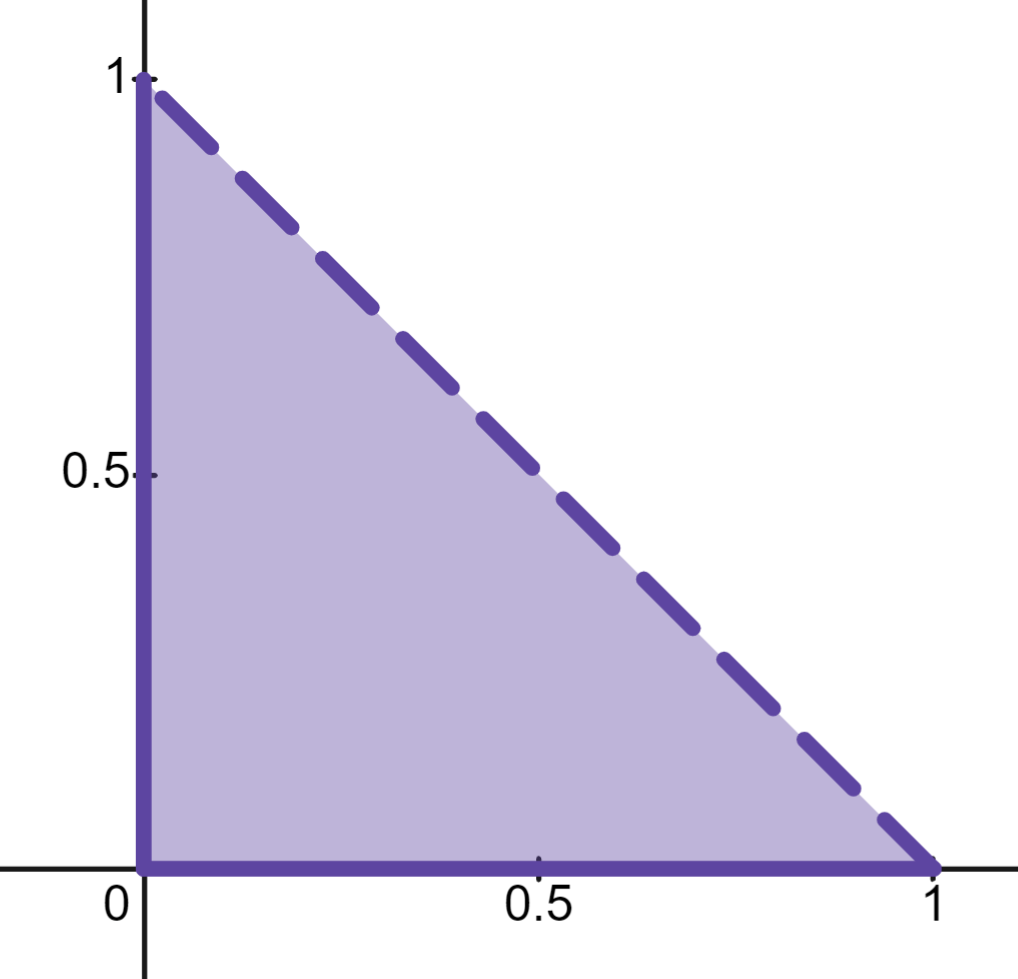
\includegraphics[scale=0.2]{140C_image_1.png}}\par}
   
            \end{tabular}
         \end{myIndent}

         Now let $\mathcal{I}$ be any set of intervals contained in $T$. By expanding\\ all the intervals when possible, we can assume without loss of\\ generality that all intervals in $\mathcal{I}$ have the form $[0, t)\times [0, 1-t)$.\retTwo

         Then, to show that the sets in $\mathcal{I}$ do not cover all of $T$, note that\\ the union of $\mathcal{I}$ will "look" like a staircase. So, you can find points\\ "between" the steps not covered by any sets in $\mathcal{I}$ but which are\\ in $T$.
         
         \begin{myIndent}\exP
            I'm stressed on time so I'm not going to go into more details.\retTwo
         \end{myIndent}
      \end{myIndent}
   \end{myIndent}}

   Claim 2 (homework): If $A \in \mathcal{E}$, then $A$ is the union of a finite collection of\\ pairwise disjoint intervals.
   
   {\begin{myIndent}\exTwo
      Proof:\\ [-4pt]
      Since $A \in \mathcal{E}$, we know $A = \bigcup\limits_{i=1}^n I_i$ where each $I_i$ is an interval.\\ [-4pt]

      Then note that $A = \bigcup\limits_{i=1}^n \left(I_i - \hspace{-0.5em}\bigcup\limits_{j=i+1}^n \hspace{-0.5em}I_j\right)$ where each of the $I_i - \hspace{-0.5em}\bigcup\limits_{j=i+1}^n \hspace{-0.5em}I_j$ are\\ [-12pt] pairwise disjoint.\\ [-4pt]
      
      Also, by repeatedly applying our prior lemma, $I_i - \hspace{-0.5em}\bigcup\limits_{j=i+1}^n \hspace{-0.5em}I_j$ can be expressed\\ [-10pt] as the union of finitely many disjoint intervals.\retTwo
   \end{myIndent}}
\end{myIndent}}

Next, given any interval $I = [a_1, b_1]\times \ldots [a_p, b_p]$, let $m(I) = \prod\limits_{i=1}^p(b_i - a_i)$.\\ [-4pt]
{\begin{myTindent}\begin{myIndent}\teachComment
   Also, if any of the inequalities defining $I$ are made strict,\\ we still define $m$ the same.\retTwo
\end{myIndent}\end{myTindent}}

\newpage

Then given any $A \in \mathcal{E}$, if $\mathcal{I}$ is a collection of intervals that are pairwise disjoint\\ such that the union of the intervals in $\mathcal{I}$ equals $A$, then we define:

{\center $m(A) = \sum\limits_{I \in \mathcal{I}}m(I)$\retTwo\par}

{\begin{myIndent}\exOne
   Claim 3 (homework): Let $\mathcal{I}$ and $\mathcal{J}$ both be collections of pairwise disjoint\\ intervals such that $\bigcup\limits_{I \in \mathcal{I}}I = A = \bigcup\limits_{J \in \mathcal{J}}\hspace{-0.2em}J$.\hspace{0.2em} Then $\sum\limits_{I \in \mathcal{I}}m(I) = \sum\limits_{J \in \mathcal{J}}\hspace{-0.15em}m(J)$.\retTwo

   {\begin{myIndent}\exTwo
      Proof:\\
      Let $\mathcal{I} = \{I_1, \ldots, I_n\}$ and $\mathcal{J} = \{J_1, \ldots, J_m\}$ Then since $I_i \cap J_j \in \mathcal{E}$ for\\ all $1 \leq i \leq n$ and $1 \leq j \leq m$ and because $I_{i_1} \cap J_{j_1}$ and $I_{i_2} \cap J_{j_2}$ are\\ disjoint whenever $i_1 \neq i_2$ or $j_1 \neq j_2$, we can define a collection $\mathcal{K}$\\ satisfying that:
      \begin{itemize}
         \item $\mathcal{K}$ is a collection of pairwise disjoint intervals.
         \item Each $I_i$ and $J_j$ is the union of a subcollection of $\mathcal{K}$.
         \item $\bigcup\limits_{l \in \mathcal{K}}l = A$.\retTwo
      \end{itemize}

      Now if $l_1 \cup \ldots \cup l_k = I_i$, then clearly $m(l_1) + \ldots + m(l_k) = m(I_i)$.
      {\begin{myIndent}\exP
         To prove this, you can just use the distributive property.\retTwo
      \end{myIndent}} 
      
      So, by rearranging terms in the sum, we can say that:
      
      {\centering $\sum\limits_{I \in \mathcal{I}}m(I) = \sum\limits_{l \in \mathcal{K}}\hspace{-0.04em}m(l) = \sum\limits_{J \in \mathcal{J}}\hspace{-0.15em}m(J)$.\retTwo\par}
   \end{myIndent}}

   This tells us that $m$ is a well defined function on $\mathcal{E}$.\retTwo

   Claim 4 (homework): $m$ is additive.
   {\begin{myIndent}\exTwo
      Proof:\\
      Suppose $A$ and $B$ are disjoint and $\mathcal{I}$ and $\mathcal{J}$ are collections of pairwise\\ disjoint intervals such that $\bigcup\limits_{I \in \mathcal{I}}I = A$ and  $\bigcup\limits_{J \in \mathcal{J}}\hspace{-0.2em}J = B$.\retTwo

      Then $\mathcal{I} \cap \mathcal{J} = \emptyset$ and $\mathcal{I} \cup \mathcal{J}$ is pairwise disjoint with $\hspace{-0.5em}\bigcup\limits_{l \in \mathcal{I}\cup\mathcal{J}}\hspace{-0.6em}l = A\cup B$.\\ [-8pt] So, we can say that:

      {\centering $m(A \cup B) = \hspace{-0.5em}\sum\limits_{l \in \mathcal{I}\cup\mathcal{J}}\hspace{-0.6em}m(l) = \sum\limits_{I \in \mathcal{I}}m(I) + \sum\limits_{J \in \mathcal{J}}\hspace{-0.15em}m(J) = m(A) + m(B)$ \retTwo\par}
   \end{myIndent}}
\end{myIndent}}

\mySepTwo

A nonnegative additive set function $\phi$ defined on $\mathcal{E}$ is said to be \udefine{regular} if:

{\begin{myIndent}
   For all $A \in \mathcal{E}$ and $\varepsilon > 0$, there exists $F, G \in \mathcal{E}$ such that $F$ is closed,\\ $G$ is open, $F \subseteq A \subseteq G$, and $\phi(G) - \varepsilon \leq \phi(A) \leq \phi(F) + \varepsilon$.\retTwo

   In other words, $\phi(G) \leq \phi(A) + \varepsilon$ and $\phi(F) \geq \phi(A) - \varepsilon$.

   \newpage

   \hTwo
   Examples:
   \begin{itemize}
      \item Hopefully it is obvious to you that $m$ is regular.
      \item Let $\mathbb{R}^p = \mathbb{R}$ and $\alpha: \mathbb{R} \longrightarrow \mathbb{R}$ be a monotonically increasing function,\\ then put for all intervals in $\mathbb{R}$:
      
      {\centering $
      \begin{matrix}
         \mu([a, b)) = \alpha(b-) - \alpha(a-) \\
         \mu([a, b]) = \alpha(b+) - \alpha(a-) \\
         \mu((a, b]) = \alpha(b+) - \alpha(a+) \\
         \mu((a, b)) = \alpha(b-) - \alpha(a+)
      \end{matrix}$ \retTwo\par}

      Also, extend this $\mu$ to all of $\mathcal{E}$ the same way we extended $m$. Then\\ $\mu$ is regular (although we won't prove that).\retTwo
   \end{itemize}
\end{myIndent}}

Let $\mu$ be additive, regular, and finite on $\mathcal{E}$. Then for any $E \subset \mathbb{R}^p$ define:

{\centering $\mu^*(E) = \inf\left\{\sum\limits_{n=1}^\infty \mu(A_n) \hspace{0.3em}\middle|\hspace{0.3em} E \subset \bigcup\limits_{n=1}^\infty A_n, \text{ where each } A_n \in \mathcal{E} \text{ and is open}\right\}$ \retTwo\par}

Then, $\mu^*: \mathcal{P}(\mathbb{R}^p)\longrightarrow [0, \infty]$ is called the \udefine{outer measure} of $E$ corresponding\\ to $\mu$ (where $\mathcal{P}(\mathbb{R}^p)$ is the power set of $\mathbb{R}^p$).


{\begin{myIndent}\hTwo
   Remark 1: You can set all but finitely many $A_n = \emptyset$ in order to emulate $E$\\ being a subset of a finite open cover of $A_n$.\\ [6pt]
   Remark 2: If $E_1 \subset E_2$, then clearly $\mu^*(E_1) \leq \mu^*(E_2)$.\\ [6pt]

   \uuline{Theorem 11.8}:
   \begin{itemize}
      \item[(A)] For every $A \in \mathcal{E},\myHS \mu^*(A) = \mu(A)$.
      
      {\begin{myIndent}\hThree
         Proof:\\
         Let $A \in \mathcal{E}$ and $\varepsilon > 0$. Then because $\mu$ is regular, there exists an open\\ set $G \supseteq A$ such that $\mu(G) \leq \mu(A) + \varepsilon$. Also, $\mu^*(A) \leq \mu(G)$ as\\ $A \subseteq G \cup \emptyset \cup \emptyset \cup \ldots$. Thus, we know that $\mu^*(A) \leq \mu(A) + \varepsilon$.\retTwo

         Meanwhile, since $\mu^*(A)$ is by definition an infimum of a set, there\\ exists a sequence $(A_n)$ of open sets in $\mathcal{E}$ whose union contains $A$\\ such that:
         
         {\centering $\sum\limits_{n=1}^\infty \mu(A_n) \leq \mu^*(A) + \varepsilon$.\retTwo\par} 

         Also, by the regularity of $\mu$ there exists a closed set $F$ such that\\ $\mu(F) \geq \mu(A) - \varepsilon$. Importantly, $F$ is compact and $(A_n)$ is an open\\ cover of $F$. So $F \subset A_1 \cup \ldots \cup A_N$ for some $N$ and hence:

         {\centering{\fontsize{12}{14}\selectfont 
         \begin{tabular}{l}
            $\mu(A) \leq \mu(F) + \varepsilon \leq \mu(A_1 \cup \ldots \cup A_N) + \varepsilon$\\
            $\phantom{\mu(A) \leq \mu(F) + \varepsilon} \leq \sum\limits_{n=1}^N \mu(A_n) + \varepsilon \leq \sum\limits_{n=1}^\infty \mu(A_n) + \varepsilon \leq \mu^*(A) + 2\varepsilon $
         \end{tabular}}\par}

         \newpage

         Since $\varepsilon$ was arbitrary, we thus have that $\mu^*(A) = \mu(A)$.\retTwo
      \end{myIndent}}

      \item[(B)] If $E = \bigcup\limits_{n=1}^\infty E_n$, then $\mu^*(E) \leq \sum\limits_{n=1}^\infty \mu^*(E_n)$.
      
      \begin{myTindent}\teachComment
         This is called \udefine{$\sigma$-subadditivity}.
      \end{myTindent}

      {\begin{myIndent}\hThree
         Proof:\\ [-4pt]
         Now suppose $E = \bigcup\limits_{n=1}^\infty E_n$.\retTwo

         If $\mu^*(E_n) = +\infty$ for any $n$, then this statement is trivially true. So,\\ assume $\mu^*(E) < +\infty$ for all $n$. Then for any $\varepsilon > 0$, there are coverings\\ $(A_{n,k})$ of $E_n$ by open elementary sets such that:

         {\centering $\sum\limits_{k=1}^\infty \mu(A_{n,k}) \leq \mu^*(E_n) + 2^{-n}\varepsilon $ \retTwo\par}

         Then because all the $(A_{n,k})$'s form an open cover for $E$, we have that:
         
         {\centering{\fontsize{12.5}{14.5}\selectfont $\mu^*(E) \leq \sum\limits_{n=1}^\infty\sum\limits_{k=1}^\infty \mu(A_{n,k}) \leq \sum\limits_{n=1}^\infty \mu^*(E_n) + \frac{1}{2}\varepsilon \cdot \frac{1}{1-\frac{1}{2}} = \sum\limits_{n=1}^\infty \mu^*(E_n) + \varepsilon$}\retTwo\par}
      \end{myIndent}}
   \end{itemize}
\end{myIndent}}

\mySepTwo 

\markLecture{5/7/2024}

For any $A, B \subseteq \mathbb{R}^p$ and $\mu^*$ defined as in last lecture, we define:
\begin{itemize}
   \item $S(A, B) = (A - B) \cup (B - A)$\quad{\teachComment (This is the \udefine{symmetric difference} of $A$ and $B$.)}
   \item $d(A, B) = \mu^*(S(A, B))$.\\
\end{itemize}

Also, given any sequence $(A_n)$ of sets, we write $A_n \rightarrow A$ if $\lim\limits_{n\rightarrow \infty} d(A_n, A) = 0$.\retTwo

If there is a sequence $(A_n)$ of elementary sets such that $A_n \rightarrow A$, then we say $A$\\ is \udefine{finitely $\mu$-measurable} and write $A \in \mathfrak{M}_F(\mu)$.\retTwo 

If $A$ is the union of countably many finitely $\mu$-measurable sets, we say that $A$ is\\ \udefine{$\mu$-measurable} and write $A \in \mathfrak{M}(\mu)$.\retTwo

{\begin{myIndent}\hTwo
   \ul{Some properties of $S$}:
   \begin{itemize}
      \item[(A)] $S(A, B) = S(B, A)$ and $S(A, A) = \emptyset$.
      {\begin{myIndent}\hThree
         Hopefully this is just obvious to you.\retTwo
      \end{myIndent}}

      \item[(B)] $S(A, B) \subseteq S(A, C) \cup S(C, B)$.
      {\begin{myIndent}\hThree
         This is because $(A - B) \subseteq (A - C) \cup (C - B)$ and\\ $(B - A) \subseteq (C - A) \cup (B - C)$.
      \end{myIndent}}

      \newpage

      \item[(C)] $S(A^\comp, B^\comp) = S(A, B)$.
      {\begin{myIndent}\hThree
         This is because:
         
         {\centering{\fontsize{12}{14}\selectfont
         \begin{tabular}{l}
            $S(A^\comp, B^\comp) = (A^\comp \cap B) \cup (B^\comp \cap A)$\\$\phantom{S(B^\comp)} = (A^\comp \cup B^\comp) \cap (A \cup B) = (A \cup B) - (A \cap B)$\\$\phantom{\phantom{S(B^\comp)} = (A^\comp \cup B^\comp) \cap (A \cup B)} = (A - B) \cup (B - A) = S(A, B)$
         \end{tabular}}\retTwo\par}
      \end{myIndent}}

      \item[(D)] $S(A_1 \cup A_2,\myHS B_1 \cup B_2) \subseteq S(A_1, B_1) \cup S(A_2, B_2)$.
      {\begin{myIndent}\hThree
         This is because:
         
         {\centering{\fontsize{12}{14}\selectfont
         \begin{tabular}{l}
             $(A_1 \cup A_2) - (B_1 \cup B_2) = (A_1 - (B_1 \cup B_2)) \cup (A_2 - (B_1 \cup B_2))$\\$\phantom{aaaaaaaaaaaaaaaaaaaaaaaaaaaaaaaaa} \subseteq (A_1 - B_1) \cup (A_2 - B_2)$
         \end{tabular}}\retTwo\par}
      \end{myIndent}}

      \item[(E)] $S(A_1 \cap A_2,\myHS B_1 \cap B_2) \subseteq S(A_1, B_1) \cup S(A_2, B_2)$.
      {\begin{myIndent}\hThree
         This is because:
         
         {\centering{\fontsize{12}{14}\selectfont
         \begin{tabular}{l}
            $S(A_1 \cap A_2,\myHS B_1 \cap B_2) = S(A_1^\comp \cup A_2^\comp,\myHS B_1^\comp \cup B_2^\comp )$\\ [3pt]
            $\phantom{S(A_1 \cap A_2)m} \subseteq S(A_1^\comp, B_1^\comp) \cup S(A_2^\comp, B_2^\comp) = S(A_1, B_1) \cup S(A_2, B_2)$
         \end{tabular}}\retTwo\par}
      \end{myIndent}}

      \item[(F)] $S(A_1 - A_2,\myHS B_1 - B_2) \subseteq S(A_1, B_1) \cup S(A_2, B_2)$.
      {\begin{myIndent}\hThree
         This is because:
         
         {\centering{\fontsize{12}{14}\selectfont
         \begin{tabular}{l}
            $S(A_1 - A_2,\myHS B_1 - B_2) = S(A_1 \cap A_2^\comp,\myHS B_1 \cap B_2^\comp)$\\ $\phantom{S(A_1 - A_2,,)}\subseteq S(A_1, B_1) \cup S(A_2^\comp, B_2^\comp) = S(A_1, B_1) \cup S(A_2, B_2)$
         \end{tabular}}\\ [22pt]\par}
      \end{myIndent}}
   \end{itemize}

   \ul{Some properties of $d$}:\quad\quad {\exOne(Homework problem 5:2)}
   \begin{itemize}
      \item[(1)] $d(A, B) = d(B, A)$ and $d(A, A) = 0$.
      {\begin{myIndent}\hThree
         The first identity is true because $S(A, B) = S(B, A)$. So\\ $\mu^*(S(A, B)) = \mu^*(S(B, A))$.\retTwo

         The second identity is true because $S(A, A) = \emptyset$ and $\emptyset \in \mathcal{E}$. So,\\ $d(A, A) = \mu^*(S(A, A)) = \mu^*(\emptyset) = \mu(\emptyset) = 0$.\retTwo
      \end{myIndent}}

      \item[(2)] $d(A, B) \leq d(A, C) + d(C, B)$
      {\begin{myIndent}\hThree
         Proof:\\
         Because $S(A, B) \subseteq S(A, C) \cup S(C, B)$ and $\mu^*$ is subadditive, we\\ have that:

         {\center{\fontsize{12}{14}\selectfont
         \begin{tabular}{l}
            $d(A, B) = \mu^*(S(A, B)) \leq \mu^*(S(A, C) \cup S(C, B))$\\ $\phantom{d(A, B) = aa} \leq \mu^*(S(A,C)) + \mu^*(S(C, B)) = d(A, C) + d(C, B)$
         \end{tabular}}\retTwo\par}
      \end{myIndent}}

      \item[(3)] $d(A_1 \cup A_2, B_1 \cup B_2) \leq d(A_1, B_1) + d(A_2, B_2)$\\ $d(A_1 \cap A_2, B_1 \cap B_2) \leq d(A_1, B_1) + d(A_2, B_2)$\\ $d(A_1 \mathop{-} A_2, B_1 \mathop{-} B_2) \leq d(A_1, B_1) + d(A_2, B_2)$
      {\begin{myIndent}\hThree
         The proof of these inequalities are identical to the proof of the\\ previous property. Just use the subadditivity of $\mu^*$ and the fact\\ that:
         \begin{myIndent}
            \begin{itemize}
               \item[$\circ$] $S(A_1 \cup A_2,\myHS B_1 \cup B_2) \subseteq S(A_1, B_1) \cup S(A_2, B_2)$\\ [-16pt]
               \item[$\circ$] $S(A_1 \cap A_2,\myHS B_1 \cap B_2) \subseteq S(A_1, B_1) \cup S(A_2, B_2)$\\ [-16pt]
               \item[$\circ$] $S(A_1 \mathop{-} A_2,\myHS B_1 \mathop{-} B_2) \subseteq S(A_1, B_1) \cup S(A_2, B_2)$
            \end{itemize}
         \end{myIndent}
      \end{myIndent}}

      \newpage

      {\centering {\exOne (Not part of homework problem 5:2)} \par}

      \item[(4)] If either $\mu^*(A)$ or $\mu^*(B)$ is finite, then $|\mu^*(A) - \mu^*(B)| \leq d(A, B)$.
      {\begin{myIndent}\hThree
         Proof:\\
         Suppose $0 \leq \mu^*(B) \leq \mu^*(A)$ where $\mu^*(B)$ is finite. Then\\ $\mu^*(A) = d(A, \emptyset) \leq d(A, B) + d(B, \emptyset) = d(A, B) + \mu^*(B)$.\\ So, because $\mu^*(B)$ is finite, we know that:
         
         {\centering $\mu^*(A) - \mu^*(B) = |\mu^*(A) - \mu^*(B)| \leq d(A, B)$\retTwo\par}
         
         Meanwhile, if $0 \leq \mu^*(A) \leq \mu^*(B)$ and $\mu^*(B)$ is still finite,\\ then note that $d(B, \emptyset) \leq d(B, A) + d(A, \emptyset)$. So, because\\ $d(B, A) = d(A, B)$, we have that:
         
         {\centering $\mu^*(B) - \mu^*(A) = |\mu^*(A) - \mu^*(B)| \leq d(A, B)$\retTwo\par}

         So the identity is true if $\mu^*(B)$ is finite. Needless to say, the\\ same reasoning works for when $\mu^*(A)$ is finite.\\ [3pt]
      \end{myIndent}}
   \end{itemize}

   Now it is worth noting that $d$ isn't quite a metric on $\mathcal{P}(\mathbb{R}^p)$ since $d(A, B) = 0$\\ does not imply that $A = B$.
   {\begin{myIndent}\hThree
      To prove this, set $\mu = m$ and suppose that $A \in \mathcal{E}$ and $B = A \cup \{\mVec{p}\}$\\ where $\mVec{p} \in \mathbb{R}^p \setminus A$. Then $d(A, B) = m^*(S(A, B)) = m^*(\{\mVec{p}\}) = 0$.\retTwo
   \end{myIndent}}

   That said, if we define the equivalence relation: $A \sim B \Longleftrightarrow d(A, B) = 0$, then\\ the set $\mathcal{P}(\mathbb{R}^p)\slash_\sim$ of equivalence classes of $\sim$ is a metric space when equipped\\ with $d$. Then in that metric space, we can view $\mathfrak{M}_F(\mu)$ as the closure of $\mathcal{E}$.\retTwo\retTwo

   \uuline{Theorem 11.10}: $\mathfrak{M}(\mu)$ is a $\sigma$-ring and $\mu^*$ is countably additive on $\mathfrak{M}(\mu)$.\\ [-6pt]
   {\begin{myIndent}\hThree
      Proof:

      {\centering \ul{Part 1: Showing $\mathfrak{M}_F(\mu)$ is a ring and $\mu^*$ is additive on $\mathfrak{M}_F(\mu)$}\\[4pt]\par}

      Suppose $A, B \in \mathfrak{M}_F(\mu)$. Then choose sequences $(A_n)$ and $(B_n)$ such\\ that each $A_n, B_n \in \mathcal{E}, \myHS A_n \rightarrow A$, and $B_n \rightarrow B$.\\ [-12pt]
      
      
      \begin{tabular}{p{2in} p{3in}}
         \raisebox{-6em}{\begin{tabular}{p{1.9in}}
            Observe that:
            \begin{itemize}
               \item $A_n \cup B_n \rightarrow A \cup B$
               \item $A_n \cap B_n \rightarrow A \cap B$
               \item $A_n \mathop{-} B_n \rightarrow A \mathop{-} B$\newline\newline\newline\newline
            \end{itemize}
         \end{tabular}}
         &
         \hFour\raisebox{0em}{\begin{myClosureOne}{2.9}
            \\ [-24pt]
            To prove the first statement here, note that:
            
            {\centering 
            \begin{tabular}{l}
               $0 \leq d(A_n \cup B_n,\myHS A \cup B)$\\
               $\phantom{aaaaaa} \leq d(A_n, A) + d(B_n, B) \rightarrow 0$
            \end{tabular}\newline\par}
   
            Likewise, the other statements are proven\newline similarly.
         \end{myClosureOne}}
      \end{tabular}\\ [-54pt]

      This proves that $A, B \in \mathfrak{M}_F(\mu) \Longrightarrow A \cup B, \myHS A \mathop{-} B \in \mathfrak{M}_F(\mu)$. So,\\ $\mathfrak{M}_F(\mu)$ is a ring.\retTwo
      
      \newpage

      Also, since $d(A_n, A) \rightarrow 0$, we must have that $\mu^*(A)$ is finite. So,\\ $\mu^*(A_n) \rightarrow \mu^*(A)$ since $|\mu^*(A_n) - \mu^*(A)| \leq d(A_n, A)$. Similarly, we\\ know that $\mu^*(B_n) \rightarrow \mu^*(B), \myHS\mu^*(A_n \cup B_n) \rightarrow \mu^*(A \cup B)$ and etc.\retTwo

     Thus, because $\mu(A_n) + \mu(B_n) = \mu(A_n \cup B_n) + \mu(A_n \cap B_n)$ for all $n$\\ (see page 41), we can conclude by letting $n \rightarrow \infty$ that:

     {\centering $\mu^*(A) + \mu^*(B) = \mu^*(A \cup B) + \mu^*(A \cap B)$ \retTwo\par}

      In turn, because $\mu^*(\emptyset) = \mu(\emptyset) = 0$, we can conclude that if $A \cap B = \emptyset$,\\ then $\mu^*(A) + \mu^*(B) = \mu^*(A \cup B)$. Hence, $\mu^*$ is additive on $\mathfrak{M}_F(\mu)$.\\ [8pt]

      {\centering \ul{Part 2: Showing that $\mu^*$ is countably additive on $\mathfrak{M}(\mu)$}\\[7pt]\par}

      Lemma 1: If $A = \bigcup\limits_{n=1}^\infty A_n \in \mathfrak{M}(\mu)$ with each $A_n \in \mathfrak{M}_F(\mu)$ and\\ [-14pt]\phantom{aaaaaaaaaaaaaaaaaaaaaaaaaaaa} pairwise disjoint, then $\mu^*(A) = \sum\limits_{n=1}^\infty \mu^*(A_n)$\\ [-4pt]
      
      {\begin{myIndent}\fontsize{12}{14}\selectfont
         Suppose $A \in \mathfrak{M}(\mu)$. Then, $A$ equals the union of a countable collection\\ $(A_n)$ of sets in $\mathfrak{M}_F(\mu)$. Without loss of generality, we can also assume\\ that $(A_n)$ is pairwise disjoint.
   
         {\begin{myIndent}\hFour\fontsize{11}{13}\selectfont
            To see why this is, assume $A_n^\prime \in \mathfrak{M}_F(\mu)$ for all $n$ and $A = \bigcup\limits_{n=1}^\infty A^\prime_n$.\\ [-9pt] Then set $A_1 = A_1^\prime$ and $A_n = \bigcup\limits_{k=1}^n A_k^\prime - \bigcup\limits_{k=1}^{n-1} A_k^\prime$.\\
   
            Then, $(A_n)$ is pairwise disjoint, each $A_n \in \mathfrak{M}_F(\mu)$, and $A = \bigcup\limits_{n=1}^\infty A_n$.\\ [-2pt]
         \end{myIndent}}
   
         By theorem 11.8.B, we know that $\mu^*(A) \leq \sum\limits_{n=1}^\infty \mu^*(A_n)$.\retTwo
   
         On the other hand, because $A \supset A_1 \cup \ldots \cup A_n$ for all $n \in \mathbb{N}$ and $\mu^*$ is\\ additive on $\mathfrak{M}_F(\mu)$, we have that for all $n$:
   
         {\centering $\mu^*(A) \geq \mu^*(A_1 \cup \ldots \cup A_n) = \mu^*(A_1) + \ldots + \mu^*(A_n)$.\retTwo\par}
   
         This means $\mu^*(A) \geq \sum\limits_{n=1}^\infty \mu^*(A_n)$. And so, the lemma is proved.\retTwo
      \end{myIndent}}

      Lemma 2: $A \in \mathfrak{M}(\mu)$ and $\mu^*(A) < \infty \Longrightarrow A \in \mathfrak{M}_F(\mu)$.\\ [-12pt]
      
      {\begin{myIndent}\fontsize{12}{14}\selectfont
         Continue letting $(A_n)$ be a countable collection of disjoint sets in\\ $\mathfrak{M}_F(\mu)$ such that $A = \bigcup A_n$ and suppose $\mu^*(A)$ is finite. Then\\ define $B_n = A_1 \cup \ldots \cup B_n$ and note that:\\ [-10pt]
   
         {\centering $0 \leq d(A, B_n) = \mu^*(\hspace{-0.4em}\bigcup\limits_{i=n+1}^\infty\hspace{-0.5em} A_i) \leq \hspace{-0.4em}\sum\limits_{i=n+1}^\infty\hspace{-0.5em} \mu^*(A_i) \rightarrow 0$ as $n \rightarrow 0$. \retTwo\par}
   
         Because $B_n \rightarrow A$ and each $B_n \in \mathfrak{M}_F(\mu)$, we know that $A \in \mathfrak{M}_F(\mu)$.\retTwo
      \end{myIndent}}

      And now, it is clear that $\mu^*$ is countably additive on $\mathfrak{M}(\mu)$.\\ [-8pt]

      {\begin{myIndent}\fontsize{12}{14}\selectfont
         Suppose $A = \bigcup A_n$ where $(A_n)$ is a pairwise disjoint sequence of\\ sets in $\mathfrak{M}(\mu)$.
         
         \newpage
         
         If all $\mu^*(A_n)$ are finite, then each $A_n \in \mathfrak{M}_F(\mu)$ by lemma 2. So,\\ we know by lemma 1 that $\mu^*(A) = \sum\limits_{n=1}^\infty \mu^*(A_n)$.\retTwo

         Meanwhile, if any $\mu^*(A_n)$ is infinite, then we trivially have that\\ $\sum\limits_{n=1}^\infty \mu^*(A_n) = \infty$ and that $\mu^*(A) = \infty$ because $A_n \subseteq A$.\\ [8pt]
      \end{myIndent}}

      {\centering \ul{Part 3: Showing that $\mathfrak{M}(\mu)$ is a $\sigma$-ring}\\[7pt]\par}

      Suppose $A_n \in \mathfrak{M}(\mu)$ for all $n \in \mathbb{N}$. Then because the union of\\ countably many sets is still countable, we know that:

      {\centering $\bigcup\limits_{n=1}^\infty A_n \in \mathfrak{M}(\mu)$ \retTwo\par}

      Meanwhile, suppose that $A, B \in \mathfrak{M}(\mu)$ and that $(A_n)$ and $(B_n)$ are\\ collections of sets in $\mathfrak{M}_F(\mu)$ such that $A = \bigcup\limits_{n=1}^\infty A_n$ and $B = \bigcup\limits_{n=1}^\infty B_n$.\\ [1pt]

      Since $A_n \cap B = \bigcup\limits_{i=1}^\infty (A_n \cap B_i)$, we  know that $A_n \cap B \in \mathfrak{M}(\mu)$ for all $n$.\retTwo
      
      Furthermore, since $A_n \cap B \subseteq A_n$ and $\mu^*(A_n)$ is finite because\\ $A_n \in \mathfrak{M}_F(\mu)$ (we showed this in part 1 of the proof), we know\\ that $\mu^*(A_n \cap B)$ is finite. Hence, $A_n \cap B \in \mathfrak{M}_F(\mu)$.\retTwo

      It follows that $A - B \in \mathfrak{M}(\mu)$ because $A - B = \bigcup\limits_{n=1}^\infty(A_n - B)$. $\blacksquare$\retTwo
   \end{myIndent}}
\end{myIndent}}

The significance of this theorem is that given any additive, regular, and finite\\ set function $\mu$ defined on $\mathcal{E}$, we know that it's outer measure is a countably\\ additive set function on the $\sigma$-ring: $\mathfrak{M}(\mu)$.\retTwo

More succinctly, we can (and will) just refer to $\mu^*$ as $\mu$ since $\mu^*$ essentially\\ extends the definition of $\mu$ from $\mathcal{E}$ to all of $\mathfrak{M}(\mu)$. This extended set function is\\ called a \udefine{measure}. And when $\mu = m$, then this extended function\\ is  called the \udefine{Lebesgue measure} on $\mathbb{R}^p$.\retTwo

\exOne
\mySepTwo

Homework 5.3: A $\sigma$-ring $\mathcal{R}$ of subsets of a set $X$ is either finite or has\\ uncountably many elements.

{\begin{myIndent}\exTwo
   If $X$ is finite, than the largest possible set of subsets of $X$ is also finite. So, we\\ can assume that $X$ is infinite.

   
   \newpage

   Now, assume that $\mathcal{R}$ is countably infinite, meaning that $\mathcal{R} = \{A_1, A_2, \ldots\}$.\\ Then for all $x \in X$, we can say that $B_x = \hspace{-0.2em}\bigcap\limits_{x \in A_i}\hspace{-0.2em}A_i \in \mathcal{R}$. In turn, this means\\ [-8pt] that $\forall x, y \in X$, $\myHS B_x \cap B_y \in \mathcal{R}$.\retTwo
   
   Suppose $z \in B_x \cap B_y$. Then $B_z \subseteq B_x \cap B_y$. Also, we can prove by\\ contradiction that $x, y \in B_Z$.
   {\begin{myIndent}\exP
      If $x \notin B_z$, then $x \in B_x - B_z$ and $z \in B_x \subseteq (B_x - B_z) \not\ni z$.\\ The same thing happens if $y \notin B_z$.\retTwo
   \end{myIndent}}

   Therefore, we would have that $B_x, B_y \subseteq B_z$. And so, $B_x = B_z = B_y$.\retTwo

   Finally, let $\mathcal{F} = \{B_x \mid x \in X\}$. Since $\mathcal{F}$ is a subset of $\mathcal{R}$, we know that $\mathcal{F}$\\ can't be uncountable. Meanwhile, we also can't have that $\mathcal{F}$ is finite. This is\\ because for any $A \in \mathcal{R}$, we know that $B_x \subseteq A$ for all $x \in A$ and $A = \bigcup\limits_{x \in A}B_x$.\\ [-8pt] So if $\mathcal{F}$ is finite, then there can only be finitely many $A$ in $\mathcal{R}$.\retTwo

   Thirdly, $\mathcal{F}$ can't be countable. To see why, assume $\mathcal{F} = \{B_{x_1}, B_{x_2}, \ldots\}$.\\ Then for any $S \subseteq \mathbb{N}$, we have that $\bigcup\limits_{i\in S}B_{x_i} \in \mathcal{R}$.\retTwo
   
   But also, because $\mathcal{F}$ is pairwise disjoint, if $S \neq T \subseteq \mathbb{N}$, then $\bigcup\limits_{i\in S}B_{x_i}  \neq \bigcup\limits_{i\in T}B_{x_i}$.\\ [-8pt] Hence, there is an injective map from $\mathcal{P}(\mathbb{N})$ to $\mathcal{R}$.\retTwo
   
   So, we've shown a contradiction if $\mathcal{R}$ is countable.\retTwo
\end{myIndent}}

\mySepTwo

Let $\mathcal{E}$ be the family of elementary subsets of $\mathbb{R}$ and denote $m: \mathcal{E} \rightarrow [0, \infty)$\\ the Lebesgue set function and by $\mu^*(A)$ the outer measure of a set $A \subseteq \mathbb{R}$.  \\Also, for a scalar $t \in \mathbb{R}$, let the set $A + t = \{x + t \mid x \in A\}$.

\begin{enumerate}
   \item If $A \in \mathcal{E}$, then $m(A + t) = m(A)$ for all $t \in \mathbb{R}$.
   {\begin{myIndent}\exTwo
      If $A \in \mathcal{E}$, then there exists disjoint intervals $I_1, I_2, \ldots, I_n$ such that\\ $A = I_1 \cup I_2 \cup \ldots \cup I_n$. Then, $m(A) = m(I_1) + m(I_2) + \ldots + m(I_n)$.\retTwo

      Now note that $A + t = (I_1 + t) \cup (I_2 + t) \cup \ldots \cup (I_n + t)$. Also,\\ $(I_i + t) \cap (I_j + t) = \emptyset$ for all $i \neq j$, meaning that:
      
      {\centering $m(A + t) = m(I_1 + t) + m(I_2 + t) + \ldots + m(I_n + t)$.\retTwo\par} 

      But clearly, $m(I_i + t) = m(I_i)$ for all $1 \leq i \leq n$. So, we conclude that\\ $m(A) = m(A + t)$.\retTwo
   \end{myIndent}}

   \item If $A \in \mathbb{R}$, then $\mu^*(A + t) = \mu^*(A)$ for all $t \in \mathbb{R}$.
   {\begin{myIndent}\exTwo
      Let $\varepsilon > 0$. Then by the definition of $\mu^*(A)$, there exists a sequence\\ $(A_n)$ of open sets from $\mathcal{E}$ such that:
      
      {\centering$A \subseteq \bigcup\limits_{n=1}^\infty A_n$ and $\mu^*(A) \leq \sum\limits_{n=1}^\infty m(A_n) \leq \mu^*(A) + \varepsilon$.\par}
      
      \newpage

      Importantly, $(A_n + t)$ is also an open cover of $A + t$. So, we know\\ that:\\ [-20pt]
      
      {\centering $\mu^*(A + t) \leq \sum\limits_{n=1}^\infty m(A_n + t) = \sum\limits_{n=1}^\infty m(A_n) \leq \mu^*(A) + \varepsilon$\retTwo\par}

      Meanwhile, by the definition of $\mu^*(A + t)$ there exists a sequence\\ $(B_n)$ of open sets from $\mathcal{E}$ such that:

      {\centering$(A + t) \subseteq \bigcup\limits_{n=1}^\infty B_n$ and $\mu^*(A + t) \leq \sum\limits_{n=1}^\infty m(B_n) \leq \mu^*(A + t) + \varepsilon$.\retTwo\par}

      Then as $(B_n + (-t))$ is also an open cover of $A$, we have that:

      {\centering $\mu^*(A) \leq \sum\limits_{n=1}^\infty m(B_n + (-t)) = \sum\limits_{n=1}^\infty m(B_n) \leq \mu^*(A + t) + \varepsilon$\retTwo\par}

      And as $\varepsilon$ was arbitrary, we're now done.\retTwo
   \end{myIndent}}
\end{enumerate}

\mySepTwo\hOne

Some notes:\\ [-18pt]
\begin{itemize}
   \item[(a)] Every open set in $\mathbb{R}^p$ is the union of a countable collection of open intervals\\ (look at exercise 3.23 which we did for homework in math 140A). Thus if $A$\\ is open, then $A \in \mathfrak{M}(\mu)$.\retTwo
   
   By taking complements, we also get that every closed set is in $\mathfrak{M}(\mu)$. This\\ is because if $A$ is closed, then $A = \mathbb{R}^k - A^\comp \in \mathfrak{M}(\mu)$.\retTwo

   \item[(b)] If $A \in \mathfrak{M}(\mu)$ and $\varepsilon > 0$, then there exists a closed set $F$ and open set $G$\\ such that $F \subseteq A \subseteq G$, $\myHS\mu(G - A) < \varepsilon$, and $\mu(A - F) < \varepsilon$.
   
   \begin{myIndent}\hTwo
      The existence of $G$ satisfying this claim is immediate from our \\definition of $\mu = \mu^*$.
      {\begin{myIndent}\hThree
         Let $\varepsilon > 0$. Then we know there exists an open cover of interval $(E_n)$\\ such that $A \subseteq \bigcup\limits_{n=1}^\infty E_n$ and $\sum\limits_{n=1}^\infty \mu(E_n) < \mu(A) + \varepsilon$.\retTwo

         Now, letting $G = \bigcup\limits_{n=1}^\infty E_n$, we know by theorem 11.8.B that\\ [-6pt] $\mu(G) \leq \sum\limits_{n=1}^\infty \mu(E_n) < \mu(A) + \varepsilon$. Also, $G$ is open. So since\\ [1pt] $G, A \in \mathfrak{M}(\mu)$, we can say that:
         
         {\centering $\mu(A) + \mu(G - A) = \mu(G) < \mu(A) + \varepsilon$.\par}
      \end{myIndent}}

      \newpage

      Meanwhile, to get $F$ just take complements of the previous arguement\\ and note that $F^\comp - A^\comp = A - F$.\retTwo
   \end{myIndent}

   \item[(c)] $E$ is a \udefine{Borel set} if $E$ can be obtained by a countable number of operations\\ (unions, intersects, and complements) starting from open sets. The\\ collection $\mathcal{B}$ of all Borel sets in $\mathbb{R}^p$ is a $\sigma$-ring.
   
   \begin{myIndent}\hTwo
      Remarks:\\ [-20pt]
      \begin{enumerate}
         \item $\mathcal{B}$ is the smallest $\sigma$-ring which contains all open sets in $\mathbb{R}^p$.
         \item If $E \in \mathcal{B}$, then $E \in \mathfrak{M}(\mu)$ no matter what $\mu$ is by note (a).\retTwo
      \end{enumerate}
   \end{myIndent}

   \item[(d)] If $A \in \mathfrak{M}(\mu)$, then there exist Borel sets $F$ and $G$ such that $F \subseteq A \subseteq G$\\ and $\mu(G - A) = \mu(A - F) = 0$.
   
   \begin{myIndent}\hTwo
      This follows from note (b) if we take $\varepsilon = \sfrac{1}{n}$ and then take the limit\\ as $n \rightarrow \infty$.\retTwo
   \end{myIndent}

   Then as $A = F \cup (A - F)$, we also know that every set is the union of a\\ Borel set and a set of measure zero.\retTwo

   \item[(e)] The sets of measure zero form a $\sigma$-ring.
   
   \item[(f)] In the case of the Lebesgue measure, every countable set has measure\\ zero. But, there are also uncountable sets of measure zero (for example,\\ the Cantor set).
\end{itemize}

\mySepTwo

\markLecture{5/9/2024}

Let $X$ be a set. We call $X$ a \udefine{measure space} if there exists a $\sigma$-ring $\mathfrak{M}$ of\\ subsets (called \udefine{measurable sets}) of $X$ and a nonnegative countably additive\\ set function $\mu$ (called a \udefine{measure}) defined on $\mathfrak{M}$. If additionally $X \in \mathfrak{M}$, then\\ $X$ is called a \udefine{measurable space}.\retTwo

\newpage

\exOne
\mySepTwo

\textbf{Exercise 11.1}: If $f \geq 0$ and $\int_E fd\mu = 0$, then $f(x) = 0$ almost everywhere on $E$.\\ [-8pt]

{\begin{myIndent}\exTwo
   For each $n \in \mathbb{N}$, define $E_n = \{x \mid f(x) > \frac{1}{n}\} \cap E$. Then set $A = \bigcup E_n$.\\ Since $E_n \subseteq A$ for every $n$, we automatically have that $\mu(E_n) \leq \mu(A)$. So,\\ $\mu(A) = 0 \Longrightarrow \mu(E_n) = 0$ for all $n$.\\ [-6pt]

   Meanwhile, set $F_n = E_n - \bigcup\limits_{k=1}^{n-1} E_k$ for all $n$.\\ [-2pt] 
   
   Since $F_n \subseteq E_n$, we have that $\mu(F_n) \leq \mu(E_n)$. So, $\mu(E_n) = 0 \Longrightarrow \mu(F_n) = 0$.\\ Also $\bigcup F_n$ = $\bigcup E_n = A$ and $(F_n)$ is a pairwise disjoint sequence of sets. So,\\ $\mu(A) = \sum \mu(F_n)$. In turn, if $\mu(E_n) = 0$ for all $n$, then $\mu(A) = 0$.\retTwo

   Finally, note that $A = \{x \mid f(x) > 0\}$. Also, if $\mu(A) > 0$, then from the\\ prior reasoning we know there exists $N$ such that $\mu(E_N) > 0$. Then as\\ $E_N \subseteq A \subseteq E$, we have that:

   {\centering $\int_E fd\mu \geq \int_{E_N} fd\mu \geq \frac{1}{N}\mu(E_n) > 0$ \retTwo\par}

   So, we conclude that $\int_E fd\mu = 0 \Longrightarrow \mu(A) = 0$.\retTwo
\end{myIndent}}

\textbf{Exercise 11.2}: If $\int_A fd\mu = 0$ for every measurable subset $A$ of a measurable set\\ $E$, then $f(x) = 0$ almost everywhere on $E$.\\ [-6pt]

{\begin{myIndent}\exTwo
   Set $\mathcal{A} = \{x \mid f^+(x) > 0\}$ and $\mathcal{B} = \{x \mid f^-(x) > 0\}$. Then as $f^+$ and $f^-$\\ are measurable, we know that $\mathcal{A}$ and $\mathcal{B}$ are measurable. Also, $\mathcal{A} \cap \mathcal{B} = \emptyset$.\\ Hence, $\mu(\mathcal{A}) + \mu(\mathcal{B}) = \mu(\mathcal{A} \cup \mathcal{B})$ where $\mathcal{A} \cup \mathcal{B} = \{x \mid f(x) \neq 0\}$.\retTwo

   Now assume $\mu(\mathcal{A} \cup \mathcal{B}) > 0$. Then we know that at least one of $\mu(\mathcal{A})$ or\\ $\mu(\mathcal{B})$ is greater than $0$.\retTwo
   
   Consider when $\mu(\mathcal{A}) > 0$. By the previous exercise, there exists some\\ set $E_n = \{x \mid f^+(x) > \frac{1}{n}\}$ such that $\mu(E_n) > 0$. Then $E_n \subseteq E$ and:

   {\centering $\int_{E_n} f^+d\mu = \int_{E_n} fd\mu \geq \frac{1}{n}\mu(E_n) > 0$\retTwo\par}

   Similarly, when $\mu(\mathcal{B}) > 0$, then there exists some $E_m = \{x \mid f^-(x) > \frac{1}{m}\}$\\ such that $\mu(E_m) > 0$. Then $E_m \subseteq E$ and:

   {\centering $\int_{E_m} f^-d\mu = -\int_{E_m} fd\mu \leq -\frac{1}{n}\mu(E_m) < 0$\retTwo\par}

   So, we conclude that if $\int_A fd\mu = 0$ for every measurable subset $A$ of a\\ measurable set $E$, then we must have that $\mu(\mathcal{A} \cup \mathcal{B}) = 0$.\retTwo
\end{myIndent}}

\mySepTwo

\newpage

\textbf{Exercise 11.3}: If $(f_n)$ is a sequence of measurable functions, then the set of\\ points $x$ such that $(f_n(x))$ converges is measurable.\\ [-6pt]

{\begin{myIndent}\exTwo
   Let $S$ equal the set of points $x$ such that $(f_n(x))$ converges. Then note that\\ by the Cauchy criterion, if $x \in S$, then for any $\varepsilon > 0$ there must exist $N$ such\\ that $\forall n, m\geq N,\myHS |f_n(x) - f_m(x)| < \varepsilon$. Or in other words:

   {\centering $S = \bigcap\limits_{\varepsilon \in \mathbb{R}_+}\bigcup\limits_{N=1}^\infty\left(\bigcap\limits_{n=N}^\infty \bigcap\limits_{n=N}^\infty \left\{t \mid |f_n(t) - f_m(t)| < \varepsilon \right\}\right)$ \retTwo\par}

   Then since for any $\varepsilon > 0$ there exists $M$ such that $0 < \frac{1}{M} < \varepsilon$, we can say\\ that:

   {\centering $S = \bigcap\limits_{M=1}^\infty\left(\bigcup\limits_{N=1}^\infty\left(\bigcap\limits_{n=N}^\infty \bigcap\limits_{n=N}^\infty \left\{t \mid |f_n(t) - f_m(t)| < \frac{1}{M} \right\}\right)\right)$ \retTwo\par}

   And thus $S$ is measurable since $\mathfrak{M}$ is a $\sigma$-ring.
   \retTwo
\end{myIndent}}

\mySepTwo

\textbf{Exercise 11.5}: Put $g(x) = \left\{
\begin{matrix}
   0 & (0 \leq x \leq \frac{1}{2}) \\ 1 & (\frac{1}{2} \leq x \leq 1)
\end{matrix}\right.$ and $f_{2k}(x) = g(x)$\\ [2pt] and $f_{2k + 1}(x) = g(1-x)$ for all $0 \leq x \leq 1$. Then $\liminf\limits_{n\rightarrow \infty} f_n(x) = 0$\\ for all $0 \leq x \leq 1$ but $\int_0^1 f_n(x)dx = \frac{1}{2}$ for all $n \in \mathbb{N}$.\\ [-6pt]

{\begin{myIndent}\exTwo
   For $0 \leq x \leq \sfrac{1}{2},\myHS f_{2k}(x) = 0$ for all $k \in \mathbb{N}$. And as $f_n \geq 0$ for all $n$, we thus\\ have that $\liminf\limits_{n\rightarrow \infty} f_n(x) = \lim\limits_{k \rightarrow \infty} f_{2k}(x) = 0$.\retTwo

   Similarly, for $\sfrac{1}{2} \leq x \leq 1,\myHS f_{2k+1}(x) = 0$ for all $k \in \mathbb{N}$. So similarly,\\ $\liminf\limits_{n\rightarrow \infty} f_n(x) = \lim\limits_{k \rightarrow \infty} f_{2k+1}(x) = 0$.\retTwo

   That said, the fact that $\int_0^1 f_n(x)dx = \frac{1}{2}$ for every $n$ is obvious since each $f_n$ is a simple function.\retTwo
\end{myIndent}}

\mySepTwo

\textbf{Exercise 11.6}: Let $f_n(x) = \left\{
\begin{matrix}
   \frac{1}{n} & (|x| \leq n) \\ 0 & (|x| > n)
\end{matrix}\right.$\\ Then $f_n(x) \rightarrow 0$ uniformly on $\mathbb{R}$ but $\int_{-\infty}^{\infty} f_ndx = 2$ for all $n \in \mathbb{N}$.\\ [-6pt]

{\begin{myIndent}\exTwo
   (ngl what the heck is the question here?)\retTwo

   The fact that $f_n(x) \rightarrow 0$ uniformly on $\mathbb{R}$ is obvious. Also, each $f_n$ is a simple\\ [2pt] function. So $\int_{-\infty}^{\infty} f_ndx = 2$ trivially as well.
\end{myIndent}}

\newpage

\mySepTwo

\textbf{Exercise 11.8}: If $f \in \mathscr{R}$ on $[a, b]$ and $F(x) = \int_a^x f(t)dt$, then $F^\prime(x) = f(x)$\\ almost everywhere on $[a, b]$.\\ [-6pt]

{\begin{myIndent}\exTwo
   In theorem 11.33, we showed that if $f \in \mathscr{R}$, then $f$ is continuous almost\\ everywhere on $[a, b]$. Additionally, by theorem 6.20 (proposition 108 in math\\ 140B notes), we know that if $f$ is continuous at $x_0$, $F$ is differentiable at $x_0$\\ with $F^\prime(x_0) = f(x_0)$. Hence $F^\prime(x) = f(x)$ almost everywhere on $[a, b]$.\retTwo
\end{myIndent}}

\textbf{Exercise 11.9}: If $f \in \mathscr{L}$ on $[a, b]$ and $F(x) = \int_a^x fdt$, then $F$ is continuous\\ on $[a, b]$.\\ [-6pt]

{\begin{myIndent}\exTwo
   %By theorem 11.26, we know that $|f| \in \mathscr{L}$ on $[a, b]$.\\
   For any $x \in [a, b]$, define $K_x(t) = \left\{
   \begin{matrix}
      1 & (a \leq t \leq x) \\ 0 & (x < t \leq b)
   \end{matrix}\right.$\retTwo
   
   Then clearly, $|K_x(t) \cdot f(t)| \leq |f(t)|$ for all $x, t \in [a, b]$. Plus, $|f| \in \mathscr{L}$ on\\ $[a, b]$ and $K_x f$ is measurable for all $x$. So, consider any sequence $(x_n)$ of points\\ in $[a, b]$ converging to some $x \in [a, b]$. Then as $fK_{x_n} \rightarrow fK_x$ as $n \rightarrow \infty$, we\\ have by Lebesgue's dominated convergence theorem that: 
   
   {\centering$\int_a^b fK_{x_n}dt \rightarrow \int_a^b fK_xdt$ as $n \rightarrow \infty$.\retTwo\par}

   But note that $\int_a^b fK_{x_n}dt = \int_a^{x_n}fdt = F(x_n)$ and $\int_a^b fK_xdt = \int_a^x fdt = F(x)$.\\ [2pt] Thus, since $(x_n)$ is arbitrary, we can conclude that $\lim\limits_{s\rightarrow x}F(s) = F(x)$.\retTwo
\end{myIndent}}

\mySepTwo

\textbf{Exercise 11.10}: If $\mu(X) < +\infty$ and $f \in \mathscr{L}^2(\mu)$ on $X$, then $f \in \mathscr{L}(\mu)$ on $X$.\\ [-6pt]

{\begin{myIndent}\exTwo
   Let $A = \{x \mid |f(x)|^2 \geq 1\}$ and $B = \{x \mid |f(x)|^2 < 1\}$.  Then importantly\\[2pt] $A \cup B = X$ but $A \cap B = \emptyset$.\retTwo

   Now $|f(x)| \leq |f(x)|^2$ for all $x \in A$. Therefore $\int_A |f|d\mu \leq \int_A |f|^2d\mu < +\infty$.\\[2pt] Meanwhile, $\int_B |f|d\mu \leq 1 \cdot \mu(B) < +\infty$. Hence, we can conclude that\\[2pt] $\int_X|f|d\mu = \int_A|f|d\mu + \int_B|f|d\mu$ is finite.
   \retTwo
\end{myIndent}}

That said, if $\mu(X) = +\infty$, then we can have that $f \in \mathscr{L}^2(\mu)$ on $X$ but $f \notin \mathscr{L}(\mu)$\\ on $X$. For example, consider $f(x) = \frac{1}{1 + |x|}$ on $\mathbb{R}$ using the Lebesgue measure.\\ [-6pt]

{\begin{myIndent}\exTwo
   Let $s(x) = \frac{1}{2^n}$ when $x \in \left[\left(\sum\limits_{i=1}^n 2^{i-1}\right) - 2^{n-1}, \myHS \sum\limits_{i=1}^n 2^{i-1}\right]$ for all $n \in \mathbb{N}$.

   \newpage

   Then for any $N \in \mathbb{N}$, if $b = \sum\limits_{i=1}^N 2^{i-1}$, we have that $N = \int_0^b sdx \leq \int_0^b fdx$\\ [-7pt] because $s \leq f$.\\ [2pt]

   Now crucially, $N \in \mathbb{N}$ was arbitrary. And since $f(x)$ is nonnegative, we know\\ that $\int_{-\infty}^{\infty} fdx \geq \int_0^b fdx$. So, $\int_{-\infty}^{\infty}fdx = +\infty$, meaning $|f| = f \notin \mathscr{L}$ on $\mathbb{R}$.\retTwo

   Meanwhile, note that $|f(x)|^2 = \frac{1}{1 + 2|x| + x^2} \leq S(x)$ where $S$ is the simple\\ function defined by:
   
   {\centering $S(x) = \left\{
   \begin{matrix}
      \frac{1}{\lceil x \rceil^{2\vphantom{|}}} & (x \geq 0) \\ \frac{1}{\lfloor x \rfloor^{2\vphantom{|}}} & (x < 0)
   \end{matrix}\right.$\retTwo\par}

   So, $\int_{-\infty}^\infty |f|^2dx \leq \int_{-\infty}^\infty Sdx = 2\cdot \sum\limits_{n=0}^\infty \frac{1}{2^n} < +\infty$. Hence, $|f|^2 \in \mathscr{L}^2$.
   \retTwo
\end{myIndent}}

\mySepTwo

\textbf{Exercise 11.11}: If $f, g \in \mathscr{L}(\mu)$ on $X$, then let $d(f, g) = \int_X |f-g|d\mu$. Then if\\ we say $f \sim g$ when $d(f, g) = 0$, we can call ${\mathscr{L}(\mu)}/_\sim$ a metric space when\\ equipped with $d$.\\ [-11pt]

{\begin{myIndent}\exTwo
   \begin{itemize}
      \item $d(f, g) = \int_X |f-g|d\mu = \int_X |g-f|d\mu = d(g, f)$.
      \item
         $d(f, h) = \int_X |f - h|d\mu \leq \int_X (|f-g| + |g-h|)d\mu$\\ [3pt]
         $\phantom{aaaaaaaaaaaaaaa} = \int_X |f-g|d\mu + \int_X |g-h|d\mu = d(f, g) + d(g, h)$.\retTwo
   \end{itemize}
\end{myIndent}}

We claim $\mathscr{L}(\mu)/_\sim$ is a complete metric space, meaning that if $(f_n)$ is a Cauchy\\ sequence, there exists a function $f \in \mathscr{L}(\mu)$ which $(f_n)$ converges to almost\\ everywhere.\\ [-6pt]

{\begin{myIndent}\exTwo
   Proof:\\
   Let $(f_n)$ be a Cauchy sequence in $\mathscr{L}(\mu)$. Then pick a subsequence $(n_k)$ of $\mathbb{N}$\\ such that $d(f_{n_k}, f_{n_{k+1}}) = \int_X |f_{n_k} - f_{n_{k+1}}|d\mu < \frac{1}{2^k}$.\retTwo

   Thus, $\sum\limits_{k=1}^\infty \int_X|f_{n_k} - f_{n_{k+1}}|d\mu \leq 1$. And by theorem 11.30, this is equivalent to\\ [-7pt] saying that $\int_X \sum\limits_{k=1}^\infty|f_{n_k} - f_{n_{k+1}}|d\mu \leq 1$.\retTwo

   Now, since $\sum\limits_{k=1}^\infty |f_{n_k}(x) - f_{n_{k+1}}(x)|d\mu$ is non-negative, we know that\\ [-8pt] $\sum\limits_{k=1}^\infty |f_{n_k}(x) - f_{n_{k+1}}(x)|d\mu$ must be finite almost everywhere on $X$.\retTwo

   This shows that $\sum\limits_{k=1}^\infty \left(f_{n_{k+1}}(x) - f_{n_{1}}(x)\right)$ exists almost everywhere on $X$.

   \newpage

   At the same time, note that $\sum\limits_{k=1}^K f_{n_k} = f_{n_{K+1}}(x) - f_{n_1}(x)$. So:\\ [-10pt]
   
   {\centering$\lim\limits_{k\rightarrow 0}f_{n_k}(x) = \sum\limits_{k=1}^\infty \left(f_{n_{k+1}}(x) - f_{n_{1}}(x)\right) + f_{n_1}(x)$ exists almost everywhere on $X$.\retTwo\par}

   Let us define $f(x) = \lim\limits_{k\rightarrow 0}f_{n_k}(x)$ whenever that limit exists. As for when that\\ limit doesn't exist, just assign whatever value you want.\retTwo

   Next, let $\varepsilon > 0$ and pick $N$ such that $\forall n, m \geq N, \myHS \int_X |f_n - f_m|d\mu \leq \varepsilon$. Then\\ if $n_k \geq N$, we have by Fatou's theorem that:
   
   {\centering $\varepsilon \geq \liminf\limits_{i\rightarrow \infty} \int_X |f_{n_i} - f_{n_k}|d\mu \geq \int_X \left(\liminf\limits_{i\rightarrow \infty} |f_{n_i} - f_{n_k}|\right)d\mu = \int_X |f - f_{n_k}|d\mu$ \retTwo\par} 

   Thus $(f - f_{n_k}) \in \mathscr{L}(\mu)$ on $X$, which in turn means $f = (f - f_{n_k}) + f_{n_k} \in \mathscr{L}(\mu)$\\ on $X$.\retTwo

   Also, since $f_{n_k} \rightarrow f$ as $k \rightarrow \infty$ and $(f_n)$ is Cauchy, we can say that $f_n \rightarrow f$\\ because $d(f, f_n) \leq d(f, f_{n_k}) + d(f_{n_k} - f_n)$.\retTwo
\end{myIndent}}

\mySepTwo

\textbf{Exercise 11.12}: Suppose that\\ [-20pt]
\begin{itemize}
   \item[(a)] $|f(x, y)| \leq 1$ if $x, y \in [0, 1]$,\\ [-20pt]
   \item[(b)] if $x$ is fixed, $f(x, y)$ is a continuous function of $y$,\\ [-20pt]
   \item[(c)] if $y$ is fixed, $f(x, y)$ is a continuous function of $x$. 
\end{itemize}

Put $g(x) = \int_{0}^{1}f(x,y)dy$ for all $x \in [0, 1]$. Then $g$ is continuous.\\ [-6pt]

{\begin{myIndent}\exTwo
   Given any $x \in [0, 1]$, consider any sequence $(x_n)$ in $[0, 1]$ converging to $x$.\\ By assumption (b) we know that each $f_{x_n}(y) \coloneq f(x_n, y) \in \mathscr{L}$ on $[0, 1]$. Also,\\ by assumption (c) we know that $(f_{x_n}(y))$ converges to $f(x, y)$ for all $y \in [0, 1]$.\\ Hence, we have that $f_{x_n} \rightarrow f_x$ pointwise where $f_x(y) = f(x, y)$.\retTwo

   Finally, by assumption (a) we can apply Lebesgue's dominated convergence\\ theorem to get that as $n \rightarrow \infty$:

   {\centering $g(x_n) = \int_{0}^1 f(x_n, y)dy = \int_{0}^1 f_{x_n}dy \rightarrow \int_0^1 f_xdy = \int_0^1 f(x, y)dy = g(x)$ \retTwo\par}

   So, $\lim\limits_{t\rightarrow x}g(t) = g(x)$.\retTwo
\end{myIndent}}

\mySepTwo

\newpage

\textbf{(Homework 7 Problem 1)}\\ [-18pt]
\begin{itemize}
   \item If $\alpha \geq 0$, then $f(x) \coloneq x^\alpha \in \mathscr{L}$ on $(0, 1)$.\\ [-14pt]
   
   {\begin{myIndent}\exTwo
      To see why, first note that $f$ is measurable since $f$ is continuous. Also,\\ $0 \leq f(x) \leq 1$ for all $x \in (0, 1)$. So, $\int_0^1 fdx$ is bounded above by $1$ and\\ thus $f \in \mathscr{L}$.\retTwo
   \end{myIndent}}

   \item If $\alpha \leq -1$, then $f(x) \coloneq x^\alpha \notin \mathscr{L}$ on $(0, 1)$.\\ [-14pt]
   
   {\begin{myIndent}\exTwo
      To see this, first note that $x^\alpha \geq x^{-1} = \frac{1}{x}$. Then, using a similar argument\\ to that of the second part of exercise 11.11, we can show that $\int_0^1 \frac{1}{x}dx \geq n$\\ for all $n \in \mathbb{N}$. Hence, $\int_0^1 x^\alpha dx = +\infty$ and thus $x^\alpha \notin \mathscr{L}$.
      \retTwo
   \end{myIndent}}

   \item If $-1 < \alpha < 0$, then $f(x) \coloneq x^\alpha \in \mathscr{L}$ on $(0, 1)$.\\ [-14pt]
   
   {\begin{myIndent}\exTwo
      For each $s \in (0, 1)$ define $K_s(t) = \left\{
      \begin{matrix}
         0 & \text{ when } 0 < x < s \\
         1 & \text{ when } s \leq x < 1
      \end{matrix}\right.$\retTwo

      Then given any monotonically decreasing sequence $(x_n)$ in $(0, 1)$ converging\\ to $0$, we have that $(K_{x_n}f)$ is a sequence of measurable functions such that\\ $K_{x_1}f(x) \leq K_{x_2}f(x) \leq \ldots$ for all $x \in (0, 1)$. Also, $K_{x_n}f \rightarrow f$ as $n \rightarrow +\infty$.\retTwo

      So, applying Lebesgue's monotone convergence theorem we have that:
      
      {\centering $\int_0^1 fdx = \lim\limits_{n\rightarrow \infty}\int_{0}^1 K_{x_n}f dx = \lim\limits_{n\rightarrow \infty} \int_{x_n}^1 fdx = \lim\limits_{n\rightarrow \infty}\frac{1}{\alpha + 1}\left(1 - x_n^{\alpha + 1}\right) = \frac{1}{\alpha + 1}$ \retTwo\par}

      Hence, $x^\alpha \in \mathscr{L}$ on $(0, 1)$.
   \end{myIndent}}
\end{itemize}

\end{document}


%\markLecture{5/2/2024}















%  I didn't do this homework because I got really behind. A bunch of the stuff in exercise 9.14 that I did is also wrong. I just need to move on. I'm leaving it commented though in case I want to return to it later.

% \exOne
% \mySepTwo

% \textbf{Exercise 9.13}: Suppose $f$ is a differentiable mapping of $\mathbb{R}$ into $\mathbb{R}^3$ such that\\ $\|f(t)\| = 1$ for every $t$. Then $f^\prime(t) \cdot f(t) = 0$.\\ [-8pt]

% {\begin{myIndent}\exTwo
%    To prove this note that $0 = (1)^\prime = (\|f(t)\|^2)^\prime = (f(t) \cdot f(t))^\prime = 2f^\prime(t) \cdot f(t)$.\\ Hence, $f^\prime(t) \cdot f(t) = 0$. The geometric intution for this is that the path traced\\ out by $f(t)$ must be confined to the unit sphere. Therefore, $f^\prime(t)$ must always\\ be zero or perpendicular to $f(t)$.\retTwo
% \end{myIndent}}

% \mySepTwo

% \textbf{Exercise 9.14}: Define $f(0, 0) = 0$ and $f(x, y) = \frac{x^3}{x^2 + y^2}$ when $(x, y) \neq 0$.
% \begin{enumerate}
%    \item[(a)] $D_1f$ and $D_2f$ exist and are bounded on $\mathbb{R}^2$.\\ [-14pt]
   
%    {\begin{myIndent}\exTwo
%       By quotient rule, we know that when $(x, y) \neq (0, 0)$:
%       \begin{center}
%          \begin{tabular}{l c r}
%             $\bullet$ \hspace{0.3em} $(D_1f)(x, y) = \frac{x^4 + 3x^2y^2}{(x^2 + y^2)^2}$
%             & &
%             $\bullet$ \hspace{0.3em} $(D_2f)(x, y) = \frac{-2x^3y}{(x^2 + y^2)^2}$
%          \end{tabular}\retTwo
%       \end{center}

%       Therefore $0 \leq (D_1f)(x, y) = \frac{x^4 + 3x^2y^2}{x^4 + 2x^2y^2 + y^4} \leq \frac{x^4}{x^4} + \frac{3x^2y^2}{2x^2y^2} = \frac{5}{2}$\\ [3pt] and $\left|(D_2f)(x, y)\right| = \frac{x^2}{x^2 + y^2} \cdot \frac{2|x||y|}{x^2 + y^2} \leq 1 \cdot \frac{2|x||y|}{(|x| - |y|)^2 + 2|x||y|} \leq 1 \cdot 1 = 1$.\retTwo

%       Meanwhile, consider that when $(x, y) = (0, 0)$, we have that:\\
%       {\fontsize{12}{14}\selectfont$(D_1f)(0, 0) = \lim\limits_{x\rightarrow 0}\frac{\frac{x^3}{x^2 + 0} - 0}{x} = \lim\limits_{x\rightarrow 0}\frac{x}{x} = 1$} and {\fontsize{12}{14}\selectfont$(D_2f)(0, 0) = \lim\limits_{x\rightarrow 0}\frac{\frac{0}{0 + y^2} - 0}{y} = 0$}.\retTwo
%    \end{myIndent}}

%    \item[(B)] If $\mVec{u}$ is a unit vector in $\mathbb{R}^2$, then the directional derivative $(D_{\mVec{u}}f)(0, 0)$ exists\\ and it's absolute value is at most $1$.\\ [-14pt]
   
%    {\begin{myIndent}\exTwo
%       Let $\mVec{u} = (u_x + u_y)$.\\ Then {\fontsize{12}{14}\selectfont$(D_{\mVec{u}}f)(0,0) = \lim\limits_{t\rightarrow 0}\frac{\frac{(tu_x)^3}{(tu_x)^2 + (tu_y)^2} \hspace{0.1em}-\hspace{0.1em} 0}{t} = \lim\limits_{t\rightarrow 0}\frac{\frac{t^3}{t^2}\cdot\frac{u_x^3}{u_x^2 + u_y^2}}{t} = \frac{u_x^3}{u_x^2 + u_y^2} = u_x^3$}\\ [-1pt] because $\|\mVec{u}\|^2 = 1$. So, we've shown that $(D_{\mVec{u}}f)(0,0)$ exists.\retTwo

%       Also, because $|u_x| \leq 1$ we know that $|(D_{\mVec{u}}f)(0,0)| = |u_x^3| \leq 1$.\retTwo
%    \end{myIndent}}

%    \item[(C)] Let $\gamma: \mathbb{R} \longrightarrow \mathbb{R}^2$ be any differentiable mapping with $\gamma(0) = (0, 0)$ and\\ $\|\gamma^\prime(t)\| > 0$ for all $t$. Setting $g(t) = f(\gamma(t))$, we have that $g$ is differentiable\\ at all $t \in \mathbb{R}$. Furthermore, if $\gamma \in \mathscr{C}^1(\mathbb{R}, \mathbb{R}^2)$, then $g \in \mathscr{C}^1(\mathbb{R}, \mathbb{R}^2)$.\\ [-14pt]

%    {\begin{myIndent}\exTwo

%       Let $\gamma(t) = (x(t), y(t))$. Importantly, because $\gamma(t)$ is differentiable, we\\ know that $x^\prime(t)$ and $y^\prime(t)$ exist for all $t \in \mathbb{R}$. At the same time, because\\ $D_1f$ and $D_2f$ are continuous when $(x, y) \neq (0, 0)$, we know that $f^\prime$ exists\\ and is continuous when $(x, y) \neq (0, 0)$.

%       \newpage

%       Firstly, let's get the trivial case out of the way. Assume $\gamma(t_0) \neq (0, 0)$.\\ Then by chain rule we know $g^\prime(t_0) = f^\prime(\gamma(t_0))\gamma^\prime(t_0) = \nabla f(\gamma(t_0)) \cdot \gamma^\prime(t_0)$\\ because $f$ is continuously differentiable at $\gamma(t_0)$. Furthermore, if $\gamma^\prime$ is\\ continuous at $t_0$, then the above expression shows that $g^\prime$ is continuous\\ at $t_0$. This is because $f$ is continuous in an open neighborhood around\\ $\gamma(t_0)$,\hspace{0.4em} $\gamma$ is continuous around $t_0$, and $\gamma^\prime(t_0)$ is assumed to be continuous\\ around $t_0$.\retTwo

%       Now assume $\gamma(t_0) = (0, 0)$. Then observe that:
      
%       {\centering{\fontsize{12}{14}\selectfont
%       \begin{tabular}{l}
%          $\frac{f(\gamma(t)) - f(\gamma(t_0))}{t - t_0} = \frac{\frac{x^3(t)}{x^2(t) + y^(t)} - \hspace{0.2em} 0 \hspace{0.2em}}{t - t_0} = \frac{\frac{x^3(t)}{(t-t_0)^3}}{\hspace{0.2em}\frac{x^2(t) + y^2(t)}{(t-t_0)^2}\hspace{0.2em}}$\\ [6pt]
%          $\phantom{aaaaa\frac{\frac{x^3(t)}{x^2(t) + y^(t)} - \hspace{0.2em} 0 \hspace{0.2em}}{t}}  = \frac{\left(\frac{x(t) - 0}{t - t_0}\right)^3}{\left(\frac{x(t) - 0}{t - t_0}\right)^2 + \left(\frac{y(t) - 0}{t - t_0}\right)^2} = \frac{\left(\frac{x(t) - x(t_0)}{t - t_0}\right)^3}{\left(\frac{x(t) - x(t_0)}{t - t_0}\right)^2 + \left(\frac{y(t) - y(t_0)}{t - t_0}\right)^2}$
%       \end{tabular}}\retTwo\par}

%       Therefore, since $\|\gamma^\prime(t_0)\| \neq 0$ we know that:
      
%       {\centering $\lim\limits_{t \rightarrow t_0}\frac{g(t) - g(t_0)}{t - t_0} = \frac{(x^\prime(t_0))^3}{(x^\prime(t_0))^2 + (y^\prime(t_0))^2} = \frac{(x^\prime(t_0))^3}{\|\gamma^\prime(t_0)\|^2}$\retTwo\par}

%       So $g$ is differentiable at $t_0$.\retTwo

%       % Everything below this is wrong I think...

%       Finally, still assuming that $\gamma(t_0) = (0, 0)$, consider that if $\gamma^\prime$ is continuous\\ at $t_0$, then we automatically have that $\frac{(x^\prime(t))^3}{\|\gamma^\prime(t)\|^2} \rightarrow \frac{(x^\prime(t_0))^3}{\|\gamma^\prime(t_0)\|^2} = g(t_0)$ as $t \rightarrow t_0$.\\ At the same time, note that:
      
%       {\centering 
%       \begin{tabular}{l}
%          $\nabla f(\gamma(t)) \cdot \gamma^\prime(t) = \frac{x^5(t) + 3x^3(t)y^2(t) - 2x^3(t)y^2(t)}{(x^2(t) + y^2(t))^2}$\\ [7pt]
%          $\phantom{\nabla f(\gamma(t)) \cdot \gamma^\prime(t)} = \frac{x^5(t) + x^3(t)y^2(t)}{(x^2(t) + y^2(t))^2} = \frac{x^3(t)}{x^2(t) + y^2(t)}$ when $\gamma(t) \neq (0, 0)$.
%       \end{tabular} \retTwo\par}

%       Therefore, if we can only consider $t$ such that $\gamma(t) \neq (0, 0)$, \retTwo\retTwo


%       AUGGGHHHHH\\

%       Sorry I can't figure this out. It's been a lazy unproductive few weeks.


%    \end{myIndent}}
% \end{enumerate}

